\documentclass[11pt, a4paper, logo, copyright, nonumbering]{deepseek}
\usepackage{xeCJK}
\usepackage[authoryear, sort&compress, round]{natbib}
\usepackage{ulem}
\usepackage{caption}
\usepackage{xspace}
\usepackage{pifont} % http://ctan.org/pkg/pifont
\usepackage{multirow}
\usepackage{tcolorbox}
\usepackage{xltabular}
\usepackage{longtable}
\usepackage{hyperref}
\interfootnotelinepenalty=10000

\usepackage{amsfonts}
\usepackage{amsmath}
\usepackage{amssymb}
\usepackage{lineno}
\usepackage{multirow}
\usepackage{adjustbox}

\usepackage[bottom]{footmisc}
% \linenumbers

\usepackage{subfigure}
\usepackage{setspace}

% damai custom package
\usepackage{dsfont}
\usepackage{array} % 用于tabularx环境
\usepackage{tabularx} % 用于tabularx环境
\usepackage{subfigure} % 用于创建子图
\usepackage{xcolor} % 用于画有颜色的框

% ########
% 附录包
\usepackage{lipsum}  % 用于生成示例文本
\usepackage{multicol} % 引入 multicol 宏包

% \usepackage[finalizecache,cachedir=.]{minted}

\setCJKmainfont[
  BoldFont=FZHei-B01,
  ItalicFont=FZKai-Z03,
  BoldItalicFont=FZFangSong-Z02,
  SmallCapsFont=FZShuSong-Z01
]{FZShuSong-Z01}
\setCJKsansfont[AutoFakeBold=1.2, AutoFakeSlant=0.15]{FZHei-B01}
\setCJKmonofont[AutoFakeBold=1.2, AutoFakeSlant=0.15]{FZHei-B01}
\setmainfont{Times New Roman}
\setmonofont[AutoFakeBold=1.2]{LMMono10}  % or 'Fira Mono'
\setstretch{1.2}
\captionsetup{font={small,it,stretch=1.2}}
\let\oldfootnotesize\footnotesize
\renewcommand{\footnotesize}{\oldfootnotesize\itshape}

\makeatletter
\def\@BTrule[#1]{%
  \ifx\longtable\undefined
    \let\@BTswitch\@BTnormal
  \else\ifx\hline\LT@hline
    \nobreak
    \let\@BTswitch\@BLTrule
  \else
     \let\@BTswitch\@BTnormal
  \fi\fi
  \global\@thisrulewidth=#1\relax
  \ifnum\@thisruleclass=\tw@\vskip\@aboverulesep\else
  \ifnum\@lastruleclass=\z@\vskip\@aboverulesep\else
  \ifnum\@lastruleclass=\@ne\vskip\doublerulesep\fi\fi\fi
  \@BTswitch}
\makeatother

\addto\extrasenglish{
    \def\chapterautorefname{Chapter}%
    \def\sectionautorefname{Section}%
    \def\paragraphautorefname{Section}
    \def\subparagraphautorefname{Section}
    \def\paragraphautorefname{Paragraph}%
    \def\tableautorefname{Table}%
    \def\equationautorefname{Equation}%
}

\newenvironment{indentchunk}[1]%
 {\begin{list}{}%
         {\setlength{\leftmargin}{#1}}%
         \item[]%
 }
 {\end{list}}
 
\bibliographystyle{abbrvnat}
% \bibliography{main}

\reportnumber{001} % Leave blank if n/a

\renewcommand{\today}{}
% DeepSeek 67B
\newcommand{\dsvi}{DeepSeek 67B}
\newcommand{\dsvic}{DeepSeek 67B Chat}
% DeepSeek-V2
\newcommand{\dsvii}{DeepSeek-V2}
\newcommand{\dsviic}{DeepSeek-V2 Chat}
\newcommand{\dsviisft}{DeepSeek-V2 Chat (SFT)}
\newcommand{\dsviirl}{DeepSeek-V2 Chat (RL)}
\newcommand{\dsattn}{MLA}
\newcommand{\dsmoe}{DeepSeekMoE}
\newcommand{\dsviilite}{DeepSeek-V2-Lite}
% DeepSeek-V3
\newcommand{\dsviii}{DeepSeek-V3}

\title{\centering \dsviii{} 技术报告}

\author[*]{
DeepSeek-AI
\\
\small
\texttt{research@deepseek.com}
}

\input{commands.tex}

\newcommand{\fix}{\marginpar{FIX}}
\newcommand{\new}{\marginpar{NEW}}

\newcommand{\zdaxie}[1]{\textcolor[rgb]{0.545,0,0.071}{#1}}

\begin{abstract}

我们介绍 \dsviii{}，这是一个强大的 Mixture-of-Experts~(MoE) 语言模型，总参数量为 671B，每个 token 激活 37B 参数。
为实现高效推理和高性价比训练，\dsviii{} 采用 Multi-head Latent Attention~(MLA) 与 \dsmoe{} 架构，这两种架构已在 \dsvii{} 中得到充分验证。
此外，\dsviii{} 首创用于负载均衡的 auxiliary-loss-free 策略，并设置 multi-token prediction 训练目标以获得更强性能。
我们在 14.8 万亿个多样且高质量的 token 上预训练 \dsviii{}，随后通过 Supervised Fine-Tuning 和 Reinforcement Learning 阶段充分释放其能力。
全面评估表明，\dsviii{} 优于其他开源模型，并取得了可比于领先闭源模型的性能。
尽管性能优异，\dsviii{} 完整训练仅需 2.788M H800 GPU 小时。
此外，它的训练过程极其稳定。
在整个训练过程中，我们没有遇到任何不可恢复的 loss spike，也没有执行任何回滚。
模型 checkpoints 可在 \url{https://github.com/deepseek-ai/DeepSeek-V3} 获取。

\end{abstract}

\begin{document}

\maketitle

\begin{figure}[ht]
\centering
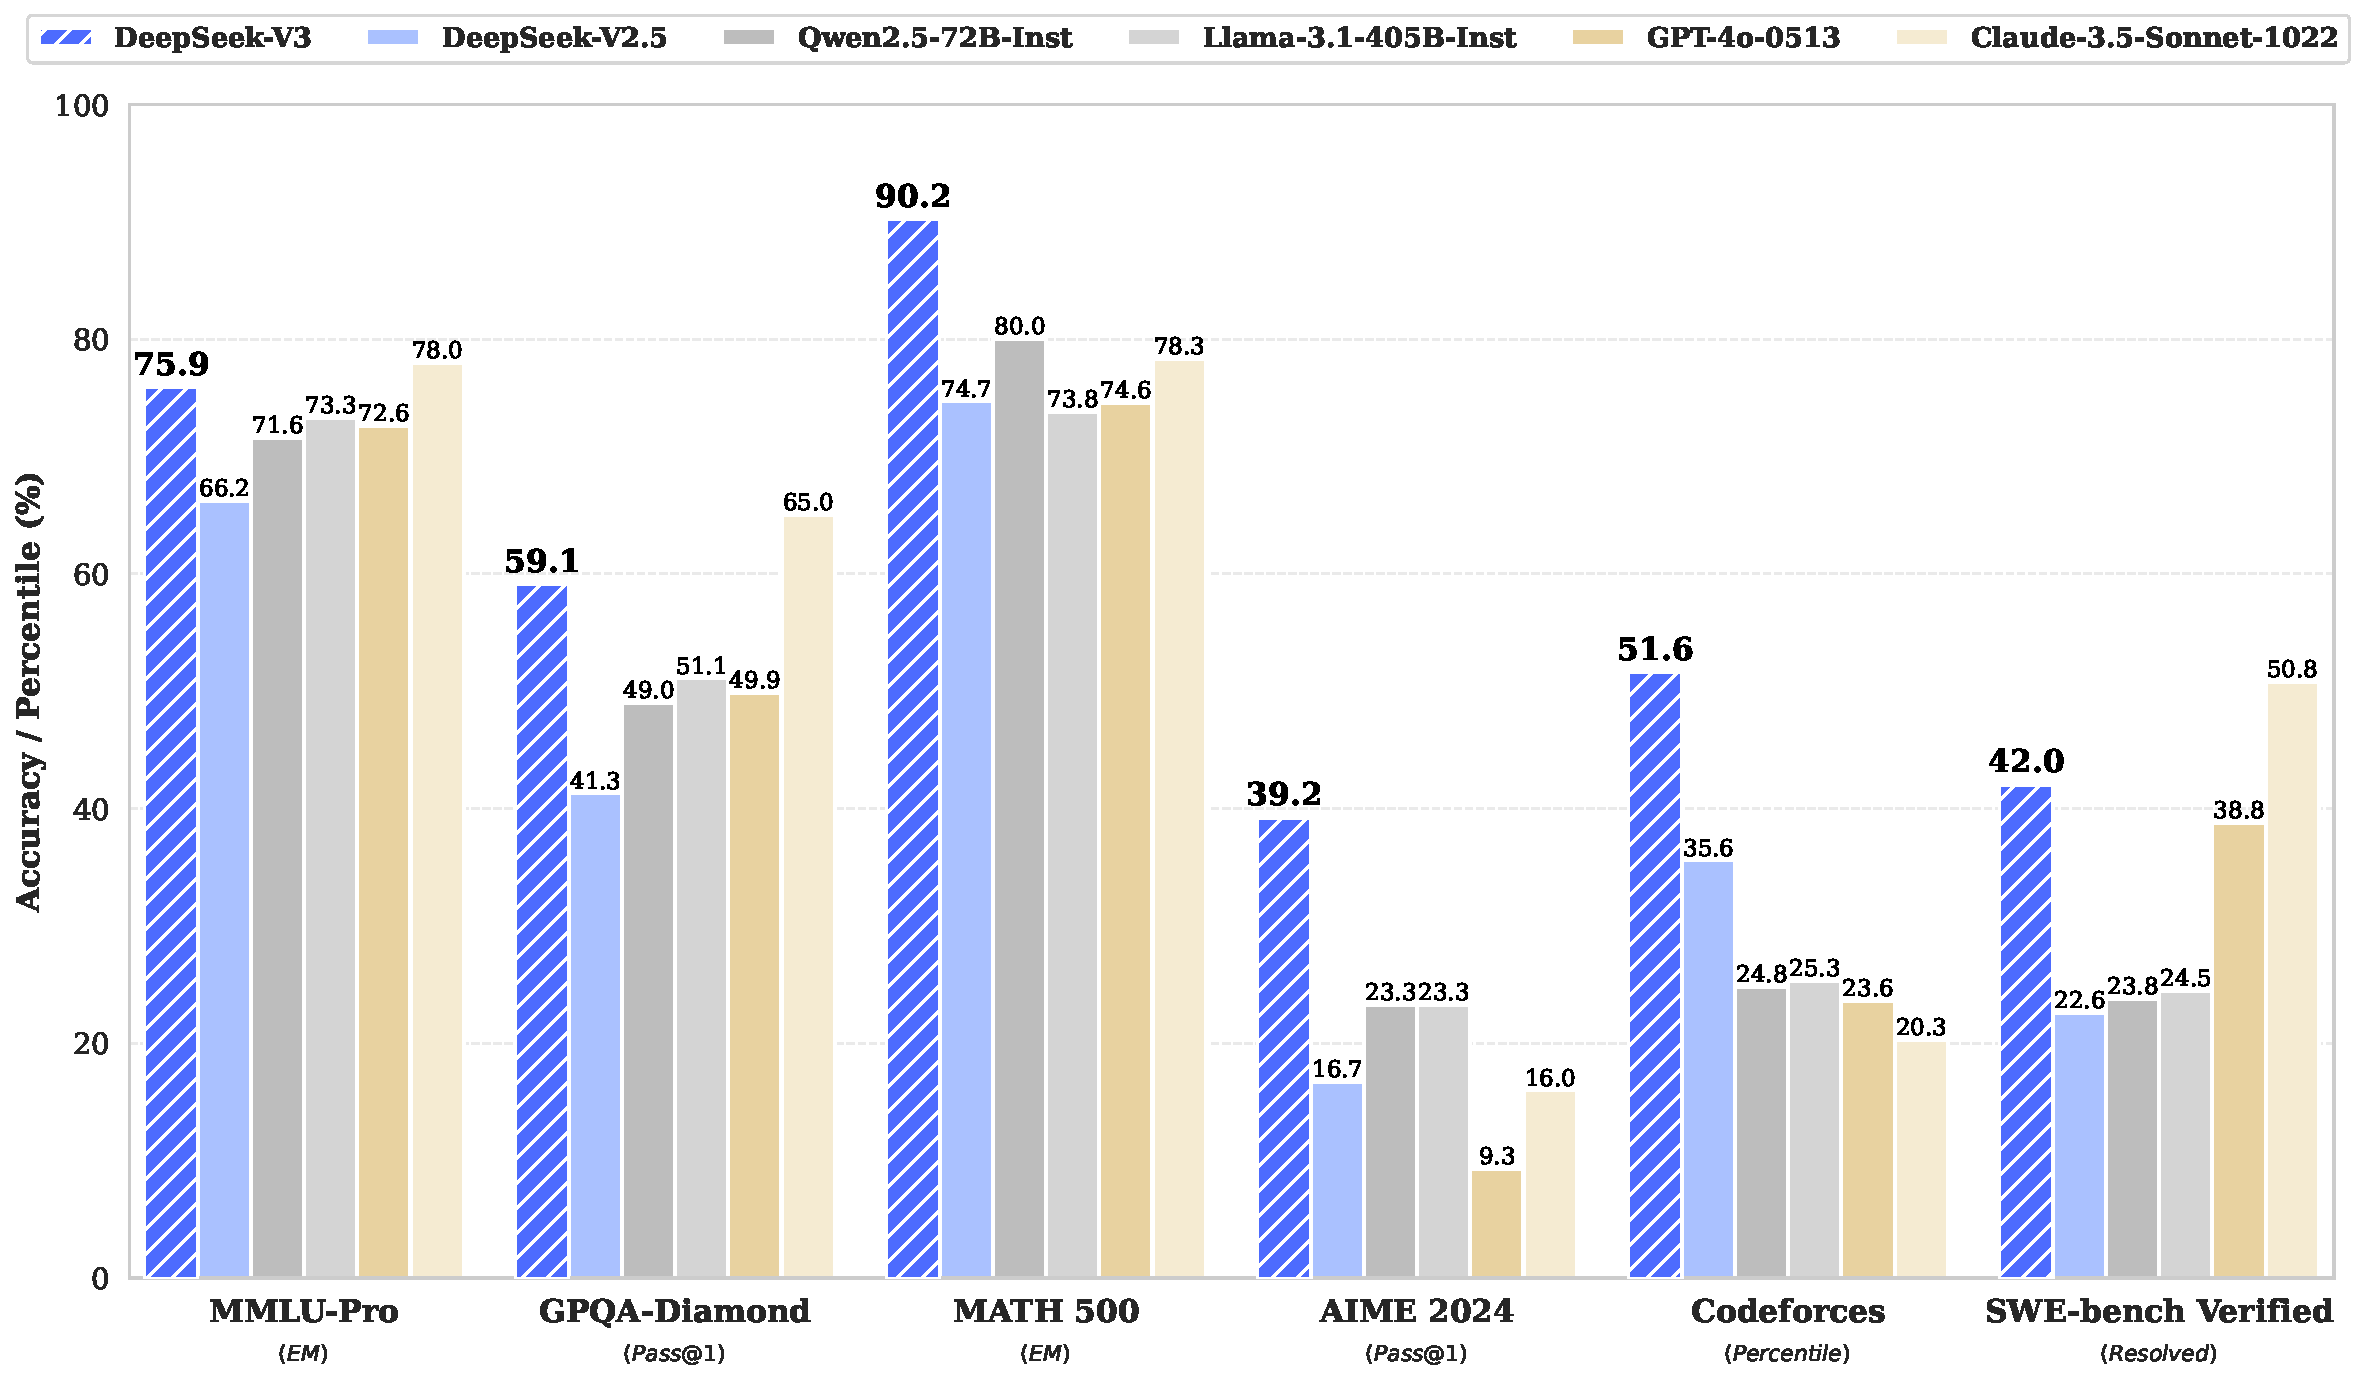
\includegraphics[width=\textwidth]{figures/dsv3_performance.pdf}
\caption{
    \centering
    \dsviii{} 及其对比模型的基准性能。
}
\label{fig:dsv3_performance}
\end{figure}

\newpage

\begin{spacing}{0.9}
\tableofcontents
\end{spacing}

\newpage

\section{引言}

近年来，Large Language Models~(LLMs) 正在快速迭代和演进~\citep{gpt4o,claude35sonnet,gemini1_5}，逐步缩小与 Artificial General Intelligence~(AGI) 的差距。
除闭源模型外，开源模型，包括 DeepSeek 系列~\citep{dsvi,dsvii,dscodervi,dscodervii}、LLaMA 系列~\citep{llama,llama2,llama3,llama3_1_405b}、Qwen 系列~\citep{qwen,qwen1_5,qwen2_5} 和 Mistral 系列~\citep{mistral,mixtral8x22b}，也在取得显著进展，努力缩小与闭源模型的差距。
为进一步推进开源模型能力边界，我们扩大模型规模并推出 \dsviii{}，这是一个拥有 671B 参数的大型 Mixture-of-Experts~(MoE) 模型，其中每个 token 激活 37B 参数。

秉持前瞻视角，我们始终追求强模型性能与低成本的结合。
因此，在架构方面，\dsviii{} 仍采用 Multi-head Latent Attention~(\dsattn{})~\citep{dsvii} 以实现高效推理，并采用 \dsmoe{}~\citep{deepseekmoe} 以实现高性价比训练。
这两种架构已在 \dsvii{}~\citep{dsvii} 中得到验证，表明它们能够在实现高效训练和推理的同时保持强劲模型性能。
在基础架构之外，我们实施了两项额外策略，以进一步增强模型能力。
首先，\dsviii{} 首创用于负载均衡的 auxiliary-loss-free 策略~\citep{noaux_tc}，旨在最大限度减少鼓励负载均衡对模型性能造成的不利影响。
其次，\dsviii{} 使用 multi-token prediction 训练目标，我们观察到它能够提升评估基准上的整体性能。

为实现高效训练，我们支持 FP8 混合精度训练，并对训练框架进行了全面优化。
低精度训练已成为高效训练的有前景方案~\citep{bf16train, fp16train, fp8lm, llm.int8}，其演进与硬件能力进步紧密相关~\citep{fp8format, hifp8format, microscaling}。
在本文中，我们介绍一个 FP8 混合精度训练框架，并首次在超大规模模型上验证其有效性。
通过支持 FP8 计算和存储，我们同时实现了训练加速与 GPU 内存使用降低。
对于训练框架，我们设计了用于高效 pipeline parallelism 的 DualPipe 算法，它具有更少的 pipeline bubbles，并通过计算与通信重叠隐藏训练期间的大部分通信。
这种重叠保证了当模型进一步扩展时，只要保持恒定的计算通信比，我们仍可跨节点使用细粒度专家，并实现近乎为零的 all-to-all 通信开销。
此外，我们还开发了高效的跨节点 all-to-all 通信 kernel，以充分利用 InfiniBand~(IB) 和 NVLink 带宽。
进一步地，我们细致优化了内存占用，使得无需使用代价高昂的 tensor parallelism 也能训练 \dsviii{}。
结合这些努力，我们实现了很高的训练效率。

在预训练期间，我们在 14.8T 个高质量且多样的 token 上训练 \dsviii{}。
预训练过程极其稳定。
在整个训练过程中，我们没有遇到任何不可恢复的 loss spike，也无需回滚。
随后，我们对 \dsviii{} 进行两阶段上下文长度扩展。第一阶段将最大上下文长度扩展到 32K，第二阶段进一步扩展到 128K。
此后，我们在 \dsviii{} 基础模型上进行 post-training，包括 Supervised Fine-Tuning~(SFT) 和 Reinforcement Learning~(RL)，以使其对齐人类偏好并进一步释放潜力。
在 post-training 阶段，我们从 DeepSeek-R1 系列模型中蒸馏推理能力，同时谨慎维持模型准确率与生成长度之间的平衡。

我们在一系列全面基准上评估 \dsviii{}。
尽管训练成本很低，全面评估表明 \dsviii{}-Base 已成为当前最强的开源基础模型，尤其在代码和数学方面表现突出。
其聊天版本也优于其他开源模型，并在一系列标准和开放式基准上取得了可比于 GPT-4o 和 Claude-3.5-Sonnet 等领先闭源模型的性能。

\begin{table}[t]
    \centering
    \setlength{\tabcolsep}{6pt}
    \begin{tabular}{l | c c c | c}
        \toprule
        \textbf{Training Costs} & \textbf{Pre-Training} & \textbf{Context Extension} & \textbf{Post-Training} & \textbf{Total} \\
        \midrule
        in H800 GPU Hours & 2664K & 119K & 5K & 2788K \\
        in USD & \$5.328M & \$0.238M & \$0.01M & \$5.576M \\
        \bottomrule
    \end{tabular}
    \caption{
    \dsviii{} 的训练成本，假设 H800 租赁价格为每 GPU 小时 \$2。
    }
    \label{tab:cost}
\end{table}

最后，我们再次强调 \dsviii{} 的低训练成本，表~\ref{tab:cost} 对此进行了总结。这一成本得益于我们对算法、框架和硬件的优化协同设计。
在预训练阶段，每训练 \dsviii{} 一万亿 token 仅需 180K H800 GPU 小时，即在我们配备 2048 块 H800 GPU 的集群上耗时 3.7 天。
因此，我们的预训练阶段在不到两个月内完成，成本为 2664K GPU 小时。
加上上下文长度扩展的 119K GPU 小时和 post-training 的 5K GPU 小时，\dsviii{} 完整训练仅耗费 2.788M GPU 小时。
假设 H800 GPU 租赁价格为每 GPU 小时 \$2，我们的总训练成本仅为 \$5.576M。
需要说明的是，上述成本仅包括 \dsviii{} 的正式训练，不包括此前在架构、算法或数据上的研究和消融实验成本。

我们的主要贡献包括：

\noindent
\textbf{架构：创新的负载均衡策略与训练目标}
\begin{itemize}[topsep=0pt]
    \item 
    在 \dsvii{} 的高效架构基础上，我们首创用于负载均衡的 auxiliary-loss-free 策略，最大限度减少鼓励负载均衡带来的性能下降。
    \item 
    我们研究 Multi-Token Prediction (MTP) 目标，并证明它有利于模型性能。
    它还可用于 speculative decoding，以加速推理。
\end{itemize}

\noindent
\textbf{预训练：迈向极致训练效率}
\begin{itemize}[topsep=0pt]
    \item
    我们设计了 FP8 混合精度训练框架，并首次在超大规模模型上验证了 FP8 训练的可行性和有效性。
    \item 
    通过算法、框架和硬件的协同设计，我们克服了跨节点 MoE 训练中的通信瓶颈，实现了近乎完全的计算通信重叠。
    这显著提升了训练效率并降低了训练成本，使我们能够在不增加额外开销的情况下进一步扩大模型规模。
    \item 
    我们仅以 2.664M H800 GPU 小时的低成本，在 14.8T 个 token 上完成 \dsviii{} 的预训练，得到当前最强的开源基础模型。
    预训练之后的后续训练阶段仅需 0.1M GPU 小时。
\end{itemize}

\noindent
\textbf{后训练：来自 DeepSeek-R1 的知识蒸馏}
\begin{itemize}[topsep=0pt]
    \item 
    我们提出一种创新方法，将 long-Chain-of-Thought (CoT) 模型，具体而言是 DeepSeek R1 系列中的一个模型，的推理能力蒸馏到标准 LLM 中，尤其是 \dsviii{}。
    我们的流程自然地将 R1 的验证与反思模式融入 \dsviii{}，并显著提升其推理性能。
    同时，我们也保持了对 \dsviii{} 输出风格和长度的控制。
\end{itemize}
\noindent
\textbf{核心评估结果总结}
\begin{itemize}[topsep=0pt]
    \item \textbf{知识}：
    (1) 
    在 MMLU、MMLU-Pro 和 GPQA 等教育类基准上，\dsviii{} 优于所有其他开源模型，在 MMLU 上达到 88.5，在 MMLU-Pro 上达到 75.9，在 GPQA 上达到 59.1。
    其性能可比于 GPT-4o 和 Claude-Sonnet-3.5 等领先闭源模型，缩小了该领域开源与闭源模型之间的差距。
    (2)
    在事实性基准上，\dsviii{} 在 SimpleQA 和 Chinese SimpleQA 上均展现出开源模型中的优越性能。
    尽管它在英文事实知识，SimpleQA，上落后于 GPT-4o 和 Claude-Sonnet-3.5，但在中文事实知识，Chinese SimpleQA，上超过这些模型，凸显了其在中文事实知识方面的优势。
    
    \item \textbf{代码、数学与推理}：
    (1)
    在所有非 long-CoT 开源和闭源模型中，\dsviii{} 在数学相关基准上取得 state-of-the-art 性能。
    值得注意的是，它甚至在 MATH-500 等特定基准上超过 o1-preview，展现出强大的数学推理能力。
    (2)
    在代码相关任务上，\dsviii{} 成为 LiveCodeBench 等编程竞赛基准中表现最好的模型，巩固了其在该领域的领先地位。
    对于工程相关任务，尽管 \dsviii{} 的表现略低于 Claude-Sonnet-3.5，但仍大幅领先所有其他模型，展现出在多样技术基准上的竞争力。
\end{itemize}


% [roadmap]
本文余下部分安排如下。我们首先详细介绍 \dsviii{} 的模型架构 (Section~\ref{sec:arch})。
随后，我们介绍基础设施，包括计算集群、训练框架、FP8 训练支持、推理部署策略，以及我们对未来硬件设计的建议。
接着，我们描述预训练过程，包括训练数据构建、超参数设置、长上下文扩展技术、相关评估以及若干讨论 (Section~\ref{sec:pre-training})。
之后，我们讨论 post-training 方面的工作，包括 Supervised Fine-Tuning (SFT)、Reinforcement Learning (RL)、相应评估和讨论 (Section~\ref{sec:alignment})。
最后，我们总结本文工作，讨论 \dsviii{} 的现有局限，并提出未来研究的潜在方向 (Section~\ref{sec:conclusion})。

\section{架构}
\label{sec:arch}

我们首先介绍 \dsviii{} 的基础架构，其特点是使用 Multi-head Latent Attention~(\dsattn{})~\citep{dsvii} 实现高效推理，并使用 \dsmoe{}~\citep{deepseekmoe} 实现低成本训练。
随后，我们介绍 Multi-Token Prediction (MTP) 训练目标，我们观察到它能够提升评估基准上的整体性能。
对于未明确提及的其他细节，\dsviii{} 沿用 \dsvii{}~\citep{dsvii} 的设置。

\begin{figure}[!t]
\centering
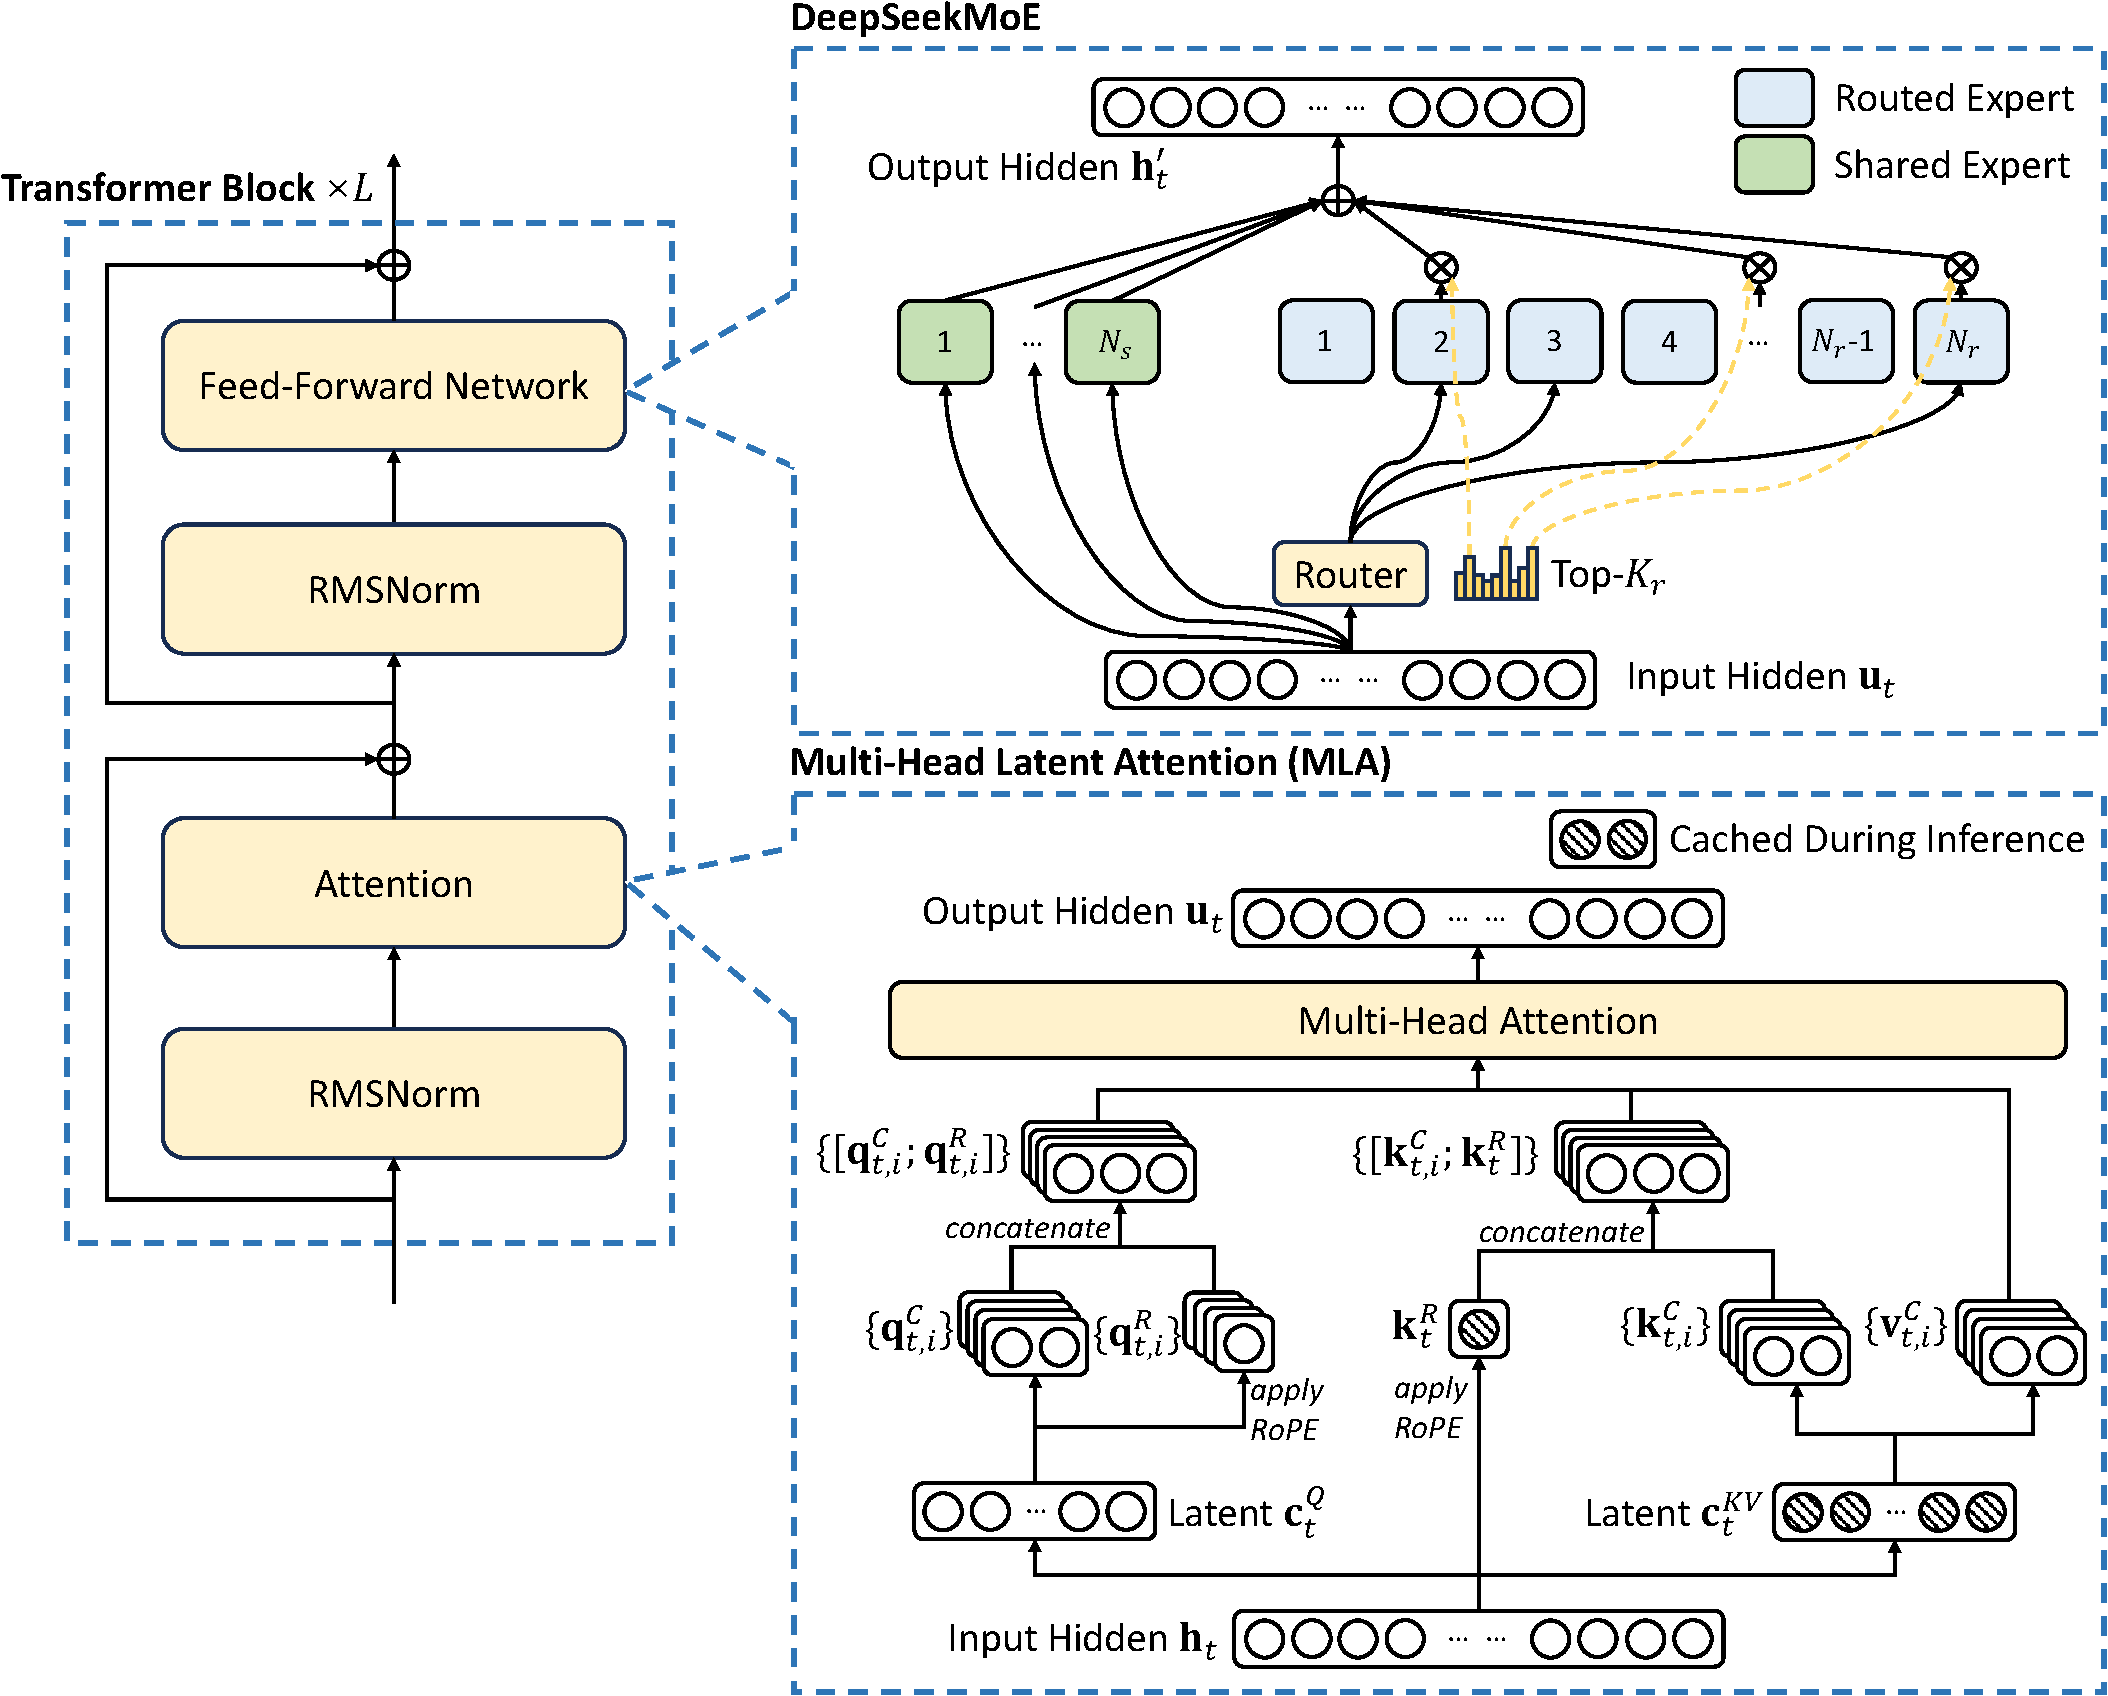
\includegraphics[width=0.99\linewidth]{figures/basic_arch.pdf}
\caption{
    \dsviii{} 基础架构示意图。
    沿袭 \dsvii{}，我们采用 \dsattn{} 和 \dsmoe{} 以实现高效推理和低成本训练。
}
\label{fig:basic_arch}
\end{figure}

\subsection{基础架构}

\dsviii{} 的基础架构仍属于 Transformer~\citep{transformer} 框架。
为实现高效推理和低成本训练，\dsviii{} 同样采用已由 \dsvii{} 充分验证的 \dsattn{} 和 \dsmoe{}。
与 \dsvii{} 相比，一个例外是我们为 \dsmoe{} 额外引入 auxiliary-loss-free 负载均衡策略~\citep{noaux_tc}，以缓解确保负载均衡所导致的性能下降。
图~\ref{fig:basic_arch} 展示了 \dsviii{} 的基础架构，本节将简要回顾 MLA 和 DeepSeekMoE 的细节。

\subsubsection{Multi-Head Latent Attention}

对于注意力，\dsviii{} 采用 \dsattn{} 架构。
令 $d$ 表示 embedding 维度，$n_h$ 表示注意力头数量，$d_h$ 表示每个头的维度，$\mathbf{h}_{t} \in \mathbb{R}^{d}$ 表示给定注意力层中第 $t$ 个 token 的注意力输入。
\dsattn{} 的核心是对注意力 key 和 value 进行低秩联合压缩，以减少推理期间的 Key-Value (KV) cache：
\begin{align}
    \boxed{\color{blue} \mathbf{c}_{t}^{KV}} &= W^{DKV} \mathbf{h}_{t}, \\
    [\mathbf{k}_{t, 1}^{C};\mathbf{k}_{t, 2}^{C};...;\mathbf{k}_{t, n_{h}}^{C}] = \mathbf{k}_{t}^{C} &= W^{UK} \mathbf{c}_{t}^{KV}, \\
    \boxed{\color{blue}\mathbf{k}_{t}^{R}} &= \operatorname{RoPE}({W^{KR}} \mathbf{h}_{t}), \\
    \mathbf{k}_{t, i} &= [\mathbf{k}_{t, i}^{C}; \mathbf{k}_{t}^{R}], \\
    [\mathbf{v}_{t, 1}^{C};\mathbf{v}_{t, 2}^{C};...;\mathbf{v}_{t, n_{h}}^{C}] = \mathbf{v}_{t}^{C} &= W^{UV} \mathbf{c}_{t}^{KV}, 
\end{align}
其中 $\mathbf{c}_{t}^{KV} \in \mathbb{R}^{d_c}$ 是 key 和 value 的压缩隐向量；
$d_c (\ll d_h n_h)$ 表示 KV 压缩维度；
$W^{DKV} \in \mathbb{R}^{d_c \times d}$ 表示下投影矩阵；
$W^{UK},W^{UV} \in \mathbb{R}^{d_h n_h \times d_c}$ 分别是 key 和 value 的上投影矩阵；
$W^{KR} \in \mathbb{R}^{d_h^R \times d}$ 是用于生成携带 Rotary Positional Embedding (RoPE)~\citep{su2024roformer} 的解耦 key 的矩阵；
$\operatorname{RoPE}(\cdot)$ 表示应用 RoPE 矩阵的操作；
$[\cdot;\cdot]$ 表示拼接。
注意，对于 MLA，生成期间只需缓存蓝框向量，即 $\color{blue} \mathbf{c}_{t}^{KV}$ 和 $\color{blue}\mathbf{k}_{t}^{R}$，因此在保持可比于标准 Multi-Head Attention (MHA)~\citep{transformer} 性能的同时，显著减少 KV cache。

对于注意力 query，我们也执行低秩压缩，这可以减少训练期间的激活内存：
\begin{align}
    \mathbf{c}_{t}^{Q} &= W^{DQ} \mathbf{h}_{t}, \\
    [\mathbf{q}_{t, 1}^{C};\mathbf{q}_{t, 2}^{C};...;\mathbf{q}_{t, n_{h}}^{C}] = \mathbf{q}_{t}^{C} &= W^{UQ} \mathbf{c}_{t}^{Q}, \\
    [\mathbf{q}_{t, 1}^{R};\mathbf{q}_{t, 2}^{R};...;\mathbf{q}_{t, n_{h}}^{R}] = \mathbf{q}_{t}^{R} &= \operatorname{RoPE}({W^{QR}} \mathbf{c}_{t}^{Q}), \\
    \mathbf{q}_{t, i} &= [\mathbf{q}_{t, i}^{C}; \mathbf{q}_{t, i}^{R}],
\end{align}
其中 $\mathbf{c}_{t}^{Q} \in \mathbb{R}^{d_c^{\prime}}$ 是 query 的压缩隐向量；
$d_c^{\prime} (\ll d_h n_h)$ 表示 query 压缩维度；
$W^{DQ} \in \mathbb{R}^{d_c^{\prime} \times d}, W^{UQ} \in \mathbb{R}^{d_h n_h \times d_c^{\prime}}$ 分别是 query 的下投影和上投影矩阵；
$W^{QR} \in \mathbb{R}^{d_h^R n_h \times d_c^{\prime}}$ 是用于生成携带 RoPE 的解耦 query 的矩阵。

最终，注意力 query ($\mathbf{q}_{t, i}$)、key ($\mathbf{k}_{j, i}$) 和 value ($\mathbf{v}_{j, i}^{C}$) 被组合起来，得到最终注意力输出 $\mathbf{u}_{t}$：
\begin{align}
    \mathbf{o}_{t, i} &= \sum_{j=1}^{t} \operatorname{Softmax}_j(\frac{\mathbf{q}_{t, i}^T \mathbf{k}_{j, i}}{\sqrt{d_{h} + d_{h}^{R}}}) \mathbf{v}_{j, i}^{C}, \\
    \mathbf{u}_{t} &= W^{O} [\mathbf{o}_{t, 1};\mathbf{o}_{t, 2};...;\mathbf{o}_{t, n_{h}}],
\end{align}
其中 $W^{O} \in \mathbb{R}^{d \times d_h n_h}$ 表示输出投影矩阵。

\subsubsection{采用 Auxiliary-Loss-Free 负载均衡的 \dsmoe{}}

\paragraph{\dsmoe{} 的基础架构。}
对于 Feed-Forward Networks~(FFNs)，\dsviii{} 使用 \dsmoe{} 架构~\citep{deepseekmoe}。
与 GShard~\citep{gshard} 等传统 MoE 架构相比，\dsmoe{} 使用更细粒度的专家，并将部分专家隔离为共享专家。
令 $\mathbf{u}_{t}$ 表示第 $t$ 个 token 的 FFN 输入，我们按如下方式计算 FFN 输出 $\mathbf{h}_{t}^{\prime}$：
\begin{align}
    \mathbf{h}_{t}^{\prime} & = \mathbf{u}_{t} + \sum_{i=1}^{N_{s}} {\operatorname{FFN}^{(s)}_{i}\left( \mathbf{u}_{t} \right)} + \sum_{i=1}^{N_r} {g_{i,t} \operatorname{FFN}^{(r)}_{i}\left( \mathbf{u}_{t} \right)}, \\
    g_{i,t} & = \frac{g^{\prime}_{i,t}}{\sum_{j=1}^{N_r} g^{\prime}_{j,t}}, \\
    g^{\prime}_{i,t} & = \begin{cases} 
    s_{i,t}, & s_{i,t} \in \operatorname{Topk} (\{ s_{j, t} | 1 \leq j \leq N_r \}, K_{r}), \\
    0, & \text{otherwise}, 
    \end{cases} \\
    s_{i,t} & = \operatorname{Sigmoid} \left( {\mathbf{u}_{t}}^{T} \mathbf{e}_{i} \right),
\end{align}
其中 $N_{s}$ 和 $N_r$ 分别表示共享专家和路由专家的数量；
$\operatorname{FFN}^{(s)}_{i}(\cdot)$ 和 $\operatorname{FFN}^{(r)}_{i}(\cdot)$ 分别表示第 $i$ 个共享专家和第 $i$ 个路由专家；
$K_{r}$ 表示被激活的路由专家数量；
$g_{i,t}$ 是第 $i$ 个专家的 gating 值；
$s_{i,t}$ 是 token-to-expert 亲和度；
$\mathbf{e}_{i}$ 是第 $i$ 个路由专家的中心向量；
$\operatorname{Topk}(\cdot, K)$ 表示由第 $t$ 个 token 与所有路由专家计算得到的亲和度分数中最高的 $K$ 个分数组成的集合。
与 \dsvii{} 略有不同，\dsviii{} 使用 sigmoid 函数计算亲和度分数，并对所有被选中的亲和度分数进行归一化以生成 gating 值。

\paragraph{Auxiliary-Loss-Free 负载均衡。}
对于 MoE 模型，不均衡的专家负载会导致 routing collapse~\citep{moe}，并在 expert parallelism 场景下降低计算效率。
传统解决方案通常依赖辅助损失~\citep{switch,gshard} 来避免负载不均衡。
然而，过大的辅助损失会损害模型性能~\citep{noaux_tc}。
为在负载均衡与模型性能之间取得更好折中，我们首创 auxiliary-loss-free 负载均衡策略~\citep{noaux_tc} 来确保负载均衡。
具体而言，我们为每个专家引入偏置项 $b_i$，并将其加到对应亲和度分数 $s_{i,t}$ 上，以确定 top-K 路由：
\begin{align}
    g^{\prime}_{i,t} & = \begin{cases} 
    s_{i,t}, & s_{i,t} + b_i \in \operatorname{Topk} (\{ s_{j, t} + b_j | 1 \leq j \leq N_r \}, K_{r}), \\
    0, & \text{otherwise}.
    \end{cases}
\end{align}
注意，偏置项仅用于路由。
将与 FFN 输出相乘的 gating 值仍由原始亲和度分数 $s_{i,t}$ 得到。
训练期间，我们持续监控每个训练 step 的整个 batch 上的专家负载。
在每个 step 结束时，如果对应专家过载，我们将其偏置项减少 $\gamma$；如果对应专家负载不足，则将其增加 $\gamma$，其中 $\gamma$ 是称为偏置更新速度的超参数。
通过这种动态调整，\dsviii{} 在训练期间保持专家负载均衡，并取得了优于仅通过辅助损失鼓励负载均衡的模型的性能。

\paragraph{互补的 Sequence-Wise 辅助损失。}
尽管 \dsviii{} 主要依赖 auxiliary-loss-free 策略实现负载均衡，为防止任意单个序列内出现极端不均衡，我们还采用了互补的 sequence-wise 平衡损失：
\begin{align}
    \mathcal{L}_{\mathrm{Bal}} & = \alpha \sum_{i=1}^{N_r}{f_i P_i}, \\
    % f_i = \frac{N_r}{K_r T} \sum_{t=1}^{T} \mathds{1}( \text{Expert $i$ } & \text{belongs to the Top-$K_r$ set for Token $t$} ), \\
    f_i = \frac{N_r}{K_r T} \sum_{t=1}^{T} \mathds{1} & \left( s_{i,t} \in \operatorname{Topk} ( \{ s_{j, t} | 1 \leq j \leq N_r \}, K_{r} ) \right), \\
    s^{\prime}_{i,t} & = \frac{s_{i,t}}{\sum_{j=1}^{N_r} s_{j,t}}, \\
    P_i & = \frac{1}{T} \sum_{t=1}^{T}{s^{\prime}_{i,t}},
\end{align}
其中平衡因子 $\alpha$ 是一个超参数，在 \dsviii{} 中被赋予极小值；
$\mathds{1}(\cdot)$ 表示指示函数；
$T$ 表示一个序列中的 token 数量。
Sequence-wise 平衡损失鼓励每个序列上的专家负载保持均衡。

\paragraph{Node-Limited Routing。}
与 \dsvii{} 使用的 device-limited routing 类似，\dsviii{} 也使用受限路由机制来限制训练期间的通信成本。
简言之，我们确保每个 token 最多发送到 $M$ 个节点，这些节点根据分布在每个节点上的专家中最高 $\frac{K_r}{M}$ 个亲和度分数之和来选择。
在该约束下，我们的 MoE 训练框架几乎可以实现完全的计算通信重叠。

\paragraph{No Token-Dropping。}
得益于有效的负载均衡策略，\dsviii{} 在完整训练期间保持了良好的负载均衡。
因此，\dsviii{} 在训练期间不会丢弃任何 token。
此外，我们还实施了特定部署策略以确保推理负载均衡，因此 \dsviii{} 在推理期间也不会丢弃 token。

\begin{figure}[!t]
\centering
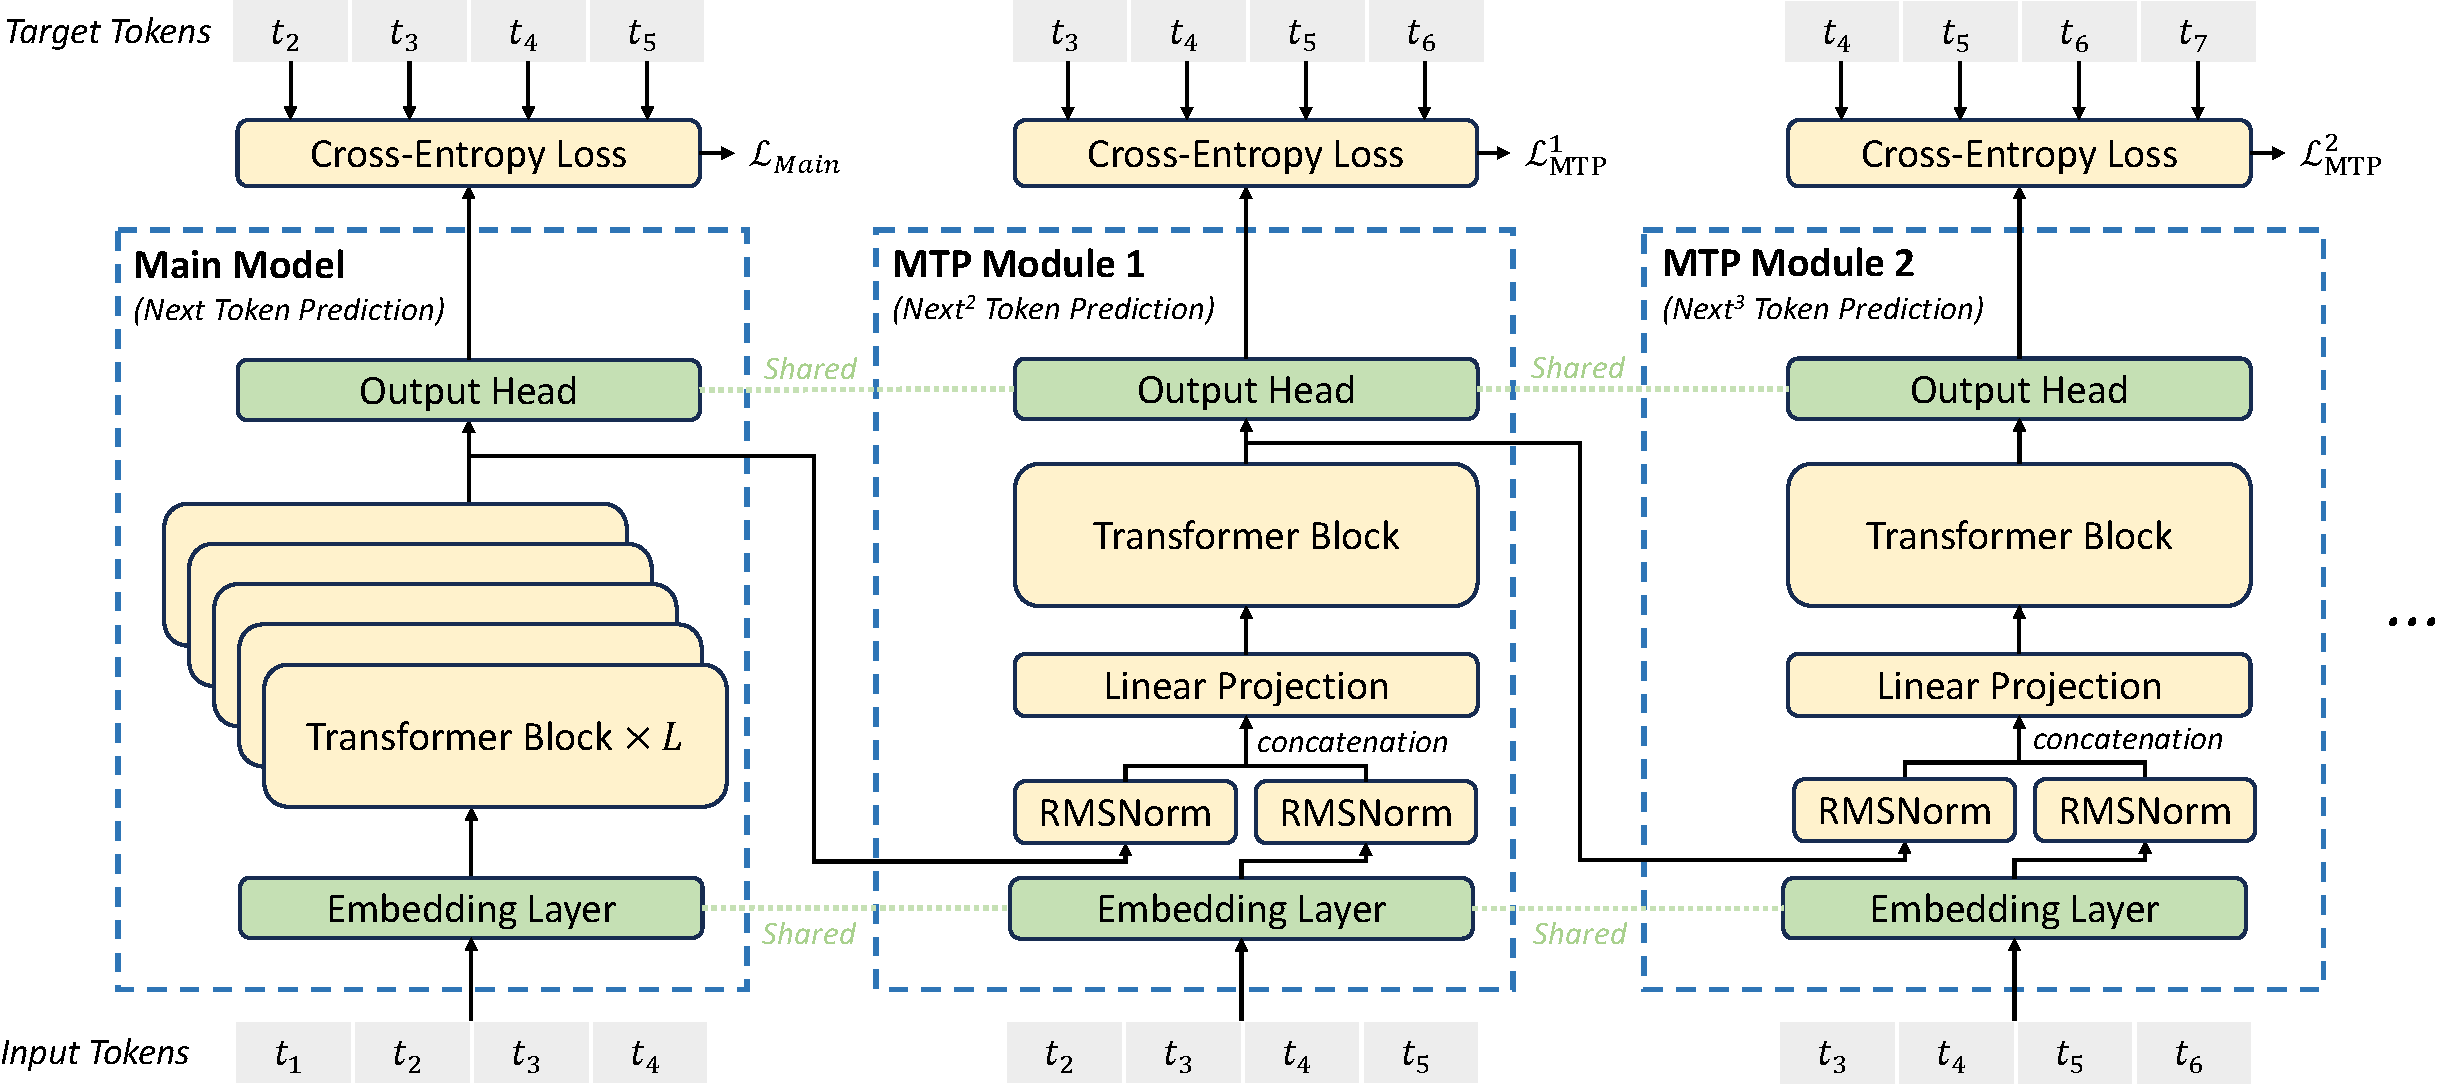
\includegraphics[width=0.99\linewidth]{figures/nextn.pdf}
\caption{
    我们的 Multi-Token Prediction (MTP) 实现示意图。
    我们在每个深度对每个 token 的预测中保留完整因果链。
}
\label{fig:nextn}
\end{figure}

\subsection{Multi-Token Prediction}

受 \citet{meta_mtp} 启发，我们为 \dsviii{} 研究并设置 Multi-Token Prediction (MTP) 目标，将每个位置的预测范围扩展到多个未来 token。
一方面，MTP 目标使训练信号更密集，并可能提升数据效率。
另一方面，MTP 可能使模型提前规划其表征，以更好预测未来 token。
图~\ref{fig:nextn} 展示了我们的 MTP 实现。
不同于 \citet{meta_mtp} 使用独立输出头并行预测 $D$ 个额外 token，我们顺序预测额外 token，并在每个预测深度保留完整因果链。
本节介绍我们 MTP 实现的细节。

\paragraph{MTP 模块。}
具体而言，我们的 MTP 实现使用 $D$ 个顺序模块来预测 $D$ 个额外 token。
第 $k$ 个 MTP 模块由共享 embedding 层 $\operatorname{Emb}(\cdot)$、共享输出头 $\operatorname{OutHead}(\cdot)$、Transformer block $\operatorname{TRM}_k(\cdot)$ 和投影矩阵 $M_k \in \mathbb{R}^{d \times 2d}$ 组成。
对于第 $i$ 个输入 token $t_i$，在第 $k$ 个预测深度，我们首先通过线性投影组合第 $i$ 个 token 在第 $(k-1)$ 个深度的表征 $\mathbf{h}_i^{k-1} \in \mathbb{R}^{d}$ 与第 $(i+k)$ 个 token 的 embedding $Emb(t_{i+k}) \in \mathbb{R}^{d}$：
\begin{equation}
    \mathbf{h}_i^{\prime k} = M_k [\operatorname{RMSNorm}(\mathbf{h}_i^{k-1}) ; \operatorname{RMSNorm}(\operatorname{Emb}(t_{i+k}))],
\end{equation}
其中 $[\cdot ; \cdot]$ 表示拼接。
特别地，当 $k=1$ 时，$\mathbf{h}_i^{k-1}$ 指主模型给出的表征。
注意，每个 MTP 模块的 embedding 层都与主模型共享。
组合后的 $\mathbf{h}_i^{\prime k}$ 作为第 $k$ 个深度处 Transformer block 的输入，用于生成当前深度的输出表征 $\mathbf{h}_{i}^{k}$：
\begin{equation}
    \mathbf{h}_{1:T-k}^{k} = \operatorname{TRM}_k(\mathbf{h}_{1:T-k}^{\prime k}),
\end{equation}
其中 $T$ 表示输入序列长度，$_{i:j}$ 表示切片操作，左右边界均包含。
最后，以 $\mathbf{h}_{i}^{k}$ 作为输入，共享输出头会计算第 $k$ 个额外预测 token 的概率分布 $P_{i+1+k}^{k} \in \mathbb{R}^{V}$，其中 $V$ 是词表大小：
\begin{equation}
    P_{i+k+1}^{k} = \operatorname{OutHead}(\mathbf{h}_{i}^{k}).
\end{equation}
输出头 $\operatorname{OutHead}(\cdot)$ 将表征线性映射为 logits，随后应用 $\operatorname{Softmax}(\cdot)$ 函数计算第 $k$ 个额外 token 的预测概率。
同样，每个 MTP 模块的输出头都与主模型共享。
我们维持预测因果链的原则与 EAGLE~\citep{eagle} 类似，但 EAGLE 的主要目标是 speculative decoding~\citep{speculative_xhm,speculative_google}，而我们使用 MTP 来改进训练。

\paragraph{MTP 训练目标。}
对于每个预测深度，我们计算交叉熵损失 $\mathcal{L}_{\text{MTP}}^{k}$：
\begin{equation}
    \mathcal{L}_{\text{MTP}}^{k} = \operatorname{CrossEntropy}(P_{2 + k:T + 1}^{k}, t_{2 + k:T + 1}) = -\frac{1}{T} \sum_{i=2 + k}^{T + 1} \log P_i^k [t_i],
\end{equation}
其中 $T$ 表示输入序列长度，$t_i$ 表示第 $i$ 个位置的 ground-truth token，$P_i^k [t_i]$ 表示由第 $k$ 个 MTP 模块给出的 $t_i$ 的对应预测概率。
最后，我们计算所有深度上 MTP 损失的平均值，并乘以权重因子 $\lambda$，得到总体 MTP 损失 $\mathcal{L}_{\text{MTP}}$，作为 \dsviii{} 的额外训练目标：
\begin{equation}
    \mathcal{L}_{\text{MTP}} = \frac{\lambda}{D} \sum_{k=1}^{D} \mathcal{L}_{\text{MTP}}^{k}.
\end{equation}

\paragraph{推理中的 MTP。}
我们的 MTP 策略主要旨在提升主模型性能，因此在推理期间，我们可以直接丢弃 MTP 模块，主模型仍可独立正常工作。
此外，我们也可以将这些 MTP 模块重新用于 speculative decoding，以进一步改善生成延迟。

\section{基础设施}
\label{sec:infra}

\subsection{计算集群}

\dsviii{} 在配备 2048 块 NVIDIA H800 GPU 的集群上训练。
H800 集群中的每个节点包含 8 块 GPU，节点内通过 NVLink 和 NVSwitch 连接。
不同节点之间使用 InfiniBand~(IB) 互连进行通信。

\subsection{训练框架}

\dsviii{} 的训练由 HAI-LLM 框架支持，这是我们的工程师从零构建的高效轻量训练框架。
总体而言，\dsviii{} 采用 16-way Pipeline Parallelism (PP)~\citep{qi2023zero}、跨 8 个节点的 64-way Expert Parallelism (EP)~\citep{gshard}，以及 ZeRO-1 Data Parallelism (DP)~\citep{zero}。

为支持 \dsviii{} 的高效训练，我们进行了细致的工程优化。
首先，我们设计了用于高效 pipeline parallelism 的 DualPipe 算法。
与现有 PP 方法相比，DualPipe 具有更少的 pipeline bubbles。
更重要的是，它在前向和反向过程中重叠计算与通信阶段，从而应对跨节点 expert parallelism 带来的重通信开销挑战。
其次，我们开发了高效的跨节点 all-to-all 通信 kernel，以充分利用 IB 和 NVLink 带宽，并节省专用于通信的 Streaming Multiprocessors (SMs)。
最后，我们细致优化训练期间的内存占用，使得无需使用昂贵的 Tensor Parallelism~(TP) 也能训练 \dsviii{}。

\subsubsection{DualPipe 与计算通信重叠}

\begin{figure}[t]
    \centering
    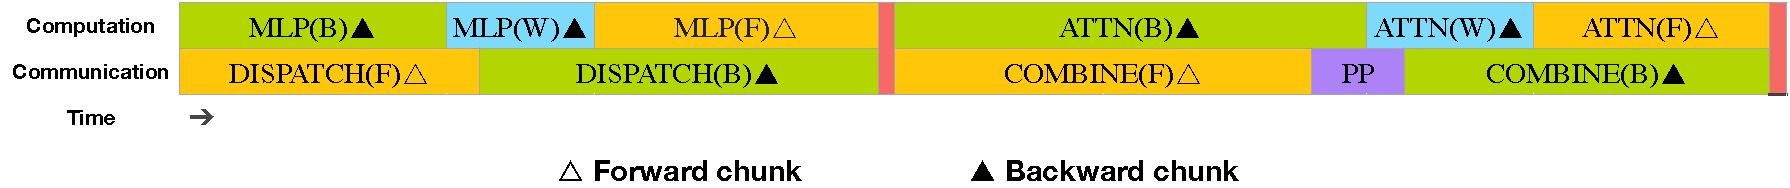
\includegraphics[width=0.9\textwidth]{figures/overlap.pdf}
    \caption{
        一对独立前向和反向 chunk 的重叠策略，transformer block 边界并未对齐。
        橙色表示前向，绿色表示 ``backward for input''，蓝色表示 ``backward for weights''，紫色表示 PP 通信，红色表示 barrier。
        all-to-all 和 PP 通信都可以被完全隐藏。
    }
    \label{fig:transformer-overlap}
\end{figure}

对于 \dsviii{}，跨节点 expert parallelism 引入的通信开销导致计算通信比低效，约为 1:1。
为应对这一挑战，我们设计了名为 DualPipe 的创新 pipeline parallelism 算法，它不仅通过有效重叠前向和反向的计算通信阶段来加速模型训练，还减少了 pipeline bubbles。

DualPipe 的核心思想是在一对独立的前向和反向 chunk 内重叠计算与通信。
具体而言，我们将每个 chunk 划分为四个组件：\texttt{attention}、\texttt{all-to-all dispatch}、\texttt{MLP} 和 \texttt{all-to-all combine}。
特别地，对于反向 chunk，\texttt{attention} 和 \texttt{MLP} 会像 ZeroBubble~\citep{zerobubble} 中一样进一步拆分为 \texttt{backward for input} 和 \texttt{backward for weights} 两部分。
此外，我们还有 \texttt{PP communication} 组件。
如图~\ref{fig:transformer-overlap} 所示，对于一对前向和反向 chunk，我们重新排列这些组件，并手动调整专用于通信与计算的 GPU SM 比例。
在这种重叠策略下，我们可以确保 all-to-all 和 PP 通信在执行期间均被完全隐藏。
基于高效的重叠策略，完整的 DualPipe 调度如图~\ref{fig:dualpipe-schedules} 所示。
它采用双向 pipeline 调度，从 pipeline 两端同时输入 micro-batch，使很大一部分通信可以被完全重叠。
这种重叠也保证了当模型进一步扩展时，只要保持恒定的计算通信比，我们仍可跨节点使用细粒度专家，并实现近乎为零的 all-to-all 通信开销。

\begin{figure}[t]
    \centering
    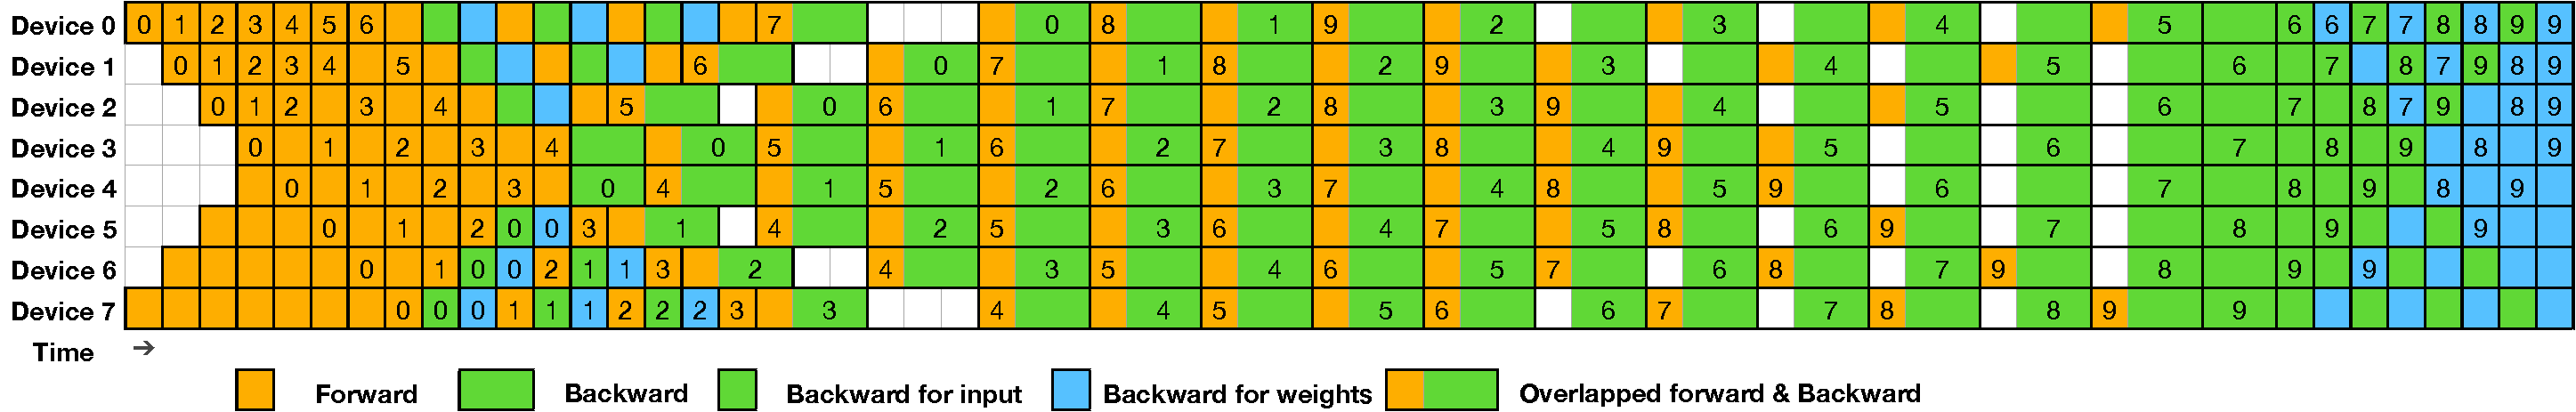
\includegraphics[width=0.99\linewidth]{figures/dualpipe.pdf}
    \caption{
        8 个 PP rank 和双向 20 个 micro-batch 的 DualPipe 调度示例。
        反向 micro-batch 与前向 micro-batch 对称，因此为简化说明，我们省略其 batch ID。
        由共享黑色边框围住的两个单元格表示计算与通信相互重叠。
    }
    \label{fig:dualpipe-schedules}
\end{figure}

此外，即便在没有重通信负担的更一般场景中，DualPipe 仍展现出效率优势。
在表~\ref{tab:dualpipe-bubble} 中，我们总结了不同 PP 方法的 pipeline bubbles 和内存使用。
如表所示，与 ZB1P~\citep{zerobubble} 和 1F1B~\citep{pipedream} 相比，DualPipe 显著减少了 pipeline bubbles，而峰值激活内存仅增加 $\frac{1}{PP}$ 倍。
尽管 DualPipe 需要保留两份模型参数，但由于训练期间使用较大的 EP size，这并不会显著增加内存消耗。
与 Chimera~\citep{chimera} 相比，DualPipe 只要求 pipeline stages 和 micro-batches 可被 2 整除，而不要求 micro-batches 可被 pipeline stages 整除。
此外，对于 DualPipe，bubbles 和激活内存都不会随着 micro-batches 数量增加而增长。

\begin{table}[t]
    \centering
    \setlength{\tabcolsep}{15pt}
    \begin{tabular}{c c c c}
        \toprule
        \textbf{Method} & \textbf{Bubble} & \textbf{Parameter} & \textbf{Activation} \\
        \midrule
        1F1B     & $(PP - 1)(F + B)$       & $1\times$ & $PP$ \\
        ZB1P     & $(PP - 1)(F + B - 2W)$   & $1\times$ & $PP$ \\
        DualPipe (Ours) & $(\frac{PP}{2} - 1)(F\&B + B - 3W)$ & $2\times$ & $PP + 1$ \\
        \bottomrule
    \end{tabular}
    \caption{
        不同 pipeline parallel 方法的 pipeline bubbles 和内存使用比较。$F$ 表示前向 chunk 的执行时间，$B$ 表示完整反向 chunk 的执行时间，$W$ 表示 ``backward for weights'' chunk 的执行时间，$F\&B$ 表示两个相互重叠的前向和反向 chunk 的执行时间。
    }
    \label{tab:dualpipe-bubble}
\end{table}

\subsubsection{跨节点 All-to-All 通信的高效实现}

为确保 DualPipe 具备充足的计算性能，我们定制了高效的跨节点 all-to-all 通信 kernel，包括 dispatching 和 combining，以节省专用于通信的 SM 数量。
这些 kernel 的实现与 MoE gating 算法以及我们集群的网络拓扑协同设计。
具体而言，在我们的集群中，跨节点 GPU 通过 IB 完全互连，节点内通信则通过 NVLink 处理。
NVLink 提供 160 GB/s 带宽，约为 IB，50 GB/s，的 3.2 倍。
为有效利用 IB 和 NVLink 的不同带宽，我们限制每个 token 最多被分发到 4 个节点，从而减少 IB 流量。
对于每个 token，当其路由决策确定后，它首先会通过 IB 传输到目标节点上具有相同节点内索引的 GPU。
到达目标节点后，我们会尽力确保它立即通过 NVLink 转发到承载目标专家的特定 GPU，而不会被随后到达的 token 阻塞。
通过这种方式，IB 和 NVLink 通信被完全重叠，每个 token 可以在不产生额外 NVLink 开销的情况下，平均每个节点高效选择 3.2 个专家。
这意味着，尽管 \dsviii{} 在实践中只选择 8 个路由专家，但在保持相同通信成本的同时，这一数量最多可以扩展到 13 个专家，4 个节点 $\times$ 3.2 个专家/节点。
总体而言，在这种通信策略下，仅 20 个 SM 就足以充分利用 IB 和 NVLink 的带宽。

具体而言，我们采用 warp specialization 技术~\citep{warp-spec}，并将 20 个 SM 划分为 10 个通信通道。
在 dispatching 过程中，(1) IB 发送，(2) IB-to-NVLink 转发，以及 (3) NVLink 接收分别由对应 warp 处理。
分配给每个通信任务的 warp 数量会根据所有 SM 上的实际工作负载动态调整。
类似地，在 combining 过程中，(1) NVLink 发送，(2) NVLink-to-IB 转发与累加，以及 (3) IB 接收与累加也由动态调整的 warp 处理。
此外，dispatching 和 combining kernel 都会与计算流重叠，因此我们也考虑它们对其他 SM 计算 kernel 的影响。
具体而言，我们使用定制 PTX (Parallel Thread Execution) 指令，并自动调优通信 chunk 大小，从而显著减少 L2 cache 使用和对其他 SM 的干扰。

\subsubsection{以极小开销大幅节省内存}

为降低训练期间的内存占用，我们采用以下技术。

\paragraph{RMSNorm 与 MLA Up-Projection 的重计算。}

我们在反向传播期间重计算所有 RMSNorm 操作和 MLA up-projections，从而无需持久存储它们的输出激活。
该策略只带来很小开销，却显著降低了存储激活所需的内存。

\paragraph{CPU 中的 Exponential Moving Average。}
训练期间，我们保留模型参数的 Exponential Moving Average (EMA)，用于在学习率衰减后早期估计模型性能。
EMA 参数存储在 CPU 内存中，并在每个训练 step 之后异步更新。
该方法使我们能够维护 EMA 参数，而不产生额外显存或时间开销。

\paragraph{Multi-Token Prediction 的共享 Embedding 与输出头。}
借助 DualPipe 策略，我们将模型最浅层，包括 embedding 层，和最深层，包括输出头，部署在同一 PP rank 上。
这种安排使 MTP 模块与主模型之间能够对共享 embedding 和输出头进行参数与梯度的物理共享。
该物理共享机制进一步提升了内存效率。

\subsection{FP8 训练}

\begin{figure}[!t]
\centering
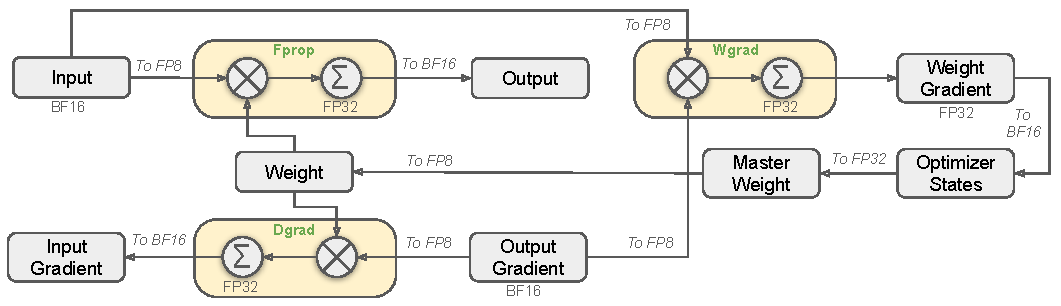
\includegraphics[width=0.99\linewidth]{figures/fp8-frameworkv3.pdf}
\caption{
    采用 FP8 数据格式的整体混合精度框架。为便于说明，图中仅展示 \texttt{Linear} 算子。
}
\label{fig:fp8_framework}
\end{figure}

受近期低精度训练进展的启发~\citep{fp8lm, llm.int8, 8-bit-numerical}，我们提出一种使用 FP8 数据格式训练 \dsviii{} 的细粒度混合精度框架。
尽管低精度训练很有前景，但它常受激活、权重和梯度中离群值的限制~\citep{massiveoutlier, understandoutlier, scalefp8train}。
虽然推理量化已取得显著进展~\citep{xiao2023smoothquant, frantar2022gptq}，但成功将低精度技术应用于大规模语言模型预训练的研究仍相对较少~\citep{scalefp8train}。
为应对这一挑战并有效扩展 FP8 格式的动态范围，我们引入一种细粒度量化策略：按包含 $1\times N_c$ 个元素的 tile 分组，或按包含 $N_c\times N_c$ 个元素的 block 分组。
在我们提高精度的累加过程中，相关的反量化开销得到大幅缓解，而这正是实现精确 FP8 General Matrix Multiplication~(GEMM) 的关键。
此外，为进一步降低 MoE 训练中的内存和通信开销，我们以 FP8 缓存和分发激活，同时以 BF16 存储低精度优化器状态。
我们在两个与 \dsvii{}-Lite 和 \dsvii{} 相近的模型规模上验证所提出的 FP8 混合精度框架，并训练约 1 万亿 token，更多细节见附录~\ref{app:fp8_cp_bf16}。
值得注意的是，与 BF16 基线相比，我们的 FP8-training 模型的相对损失误差始终低于 0.25\%，处于训练随机性可接受范围内。

\subsubsection{混合精度框架}
基于低精度训练中广泛采用的技术~\citep{bf16train, fp16train}，我们提出一个用于 FP8 训练的混合精度框架。
在该框架中，大多数计算密集型操作以 FP8 执行，而少数关键操作被有策略地保留为原始数据格式，以平衡训练效率与数值稳定性。
整体框架如图~\ref{fig:fp8_framework} 所示。

首先，为加速模型训练，大多数核心计算 kernel，即 GEMM 操作，都以 FP8 精度实现。
这些 GEMM 操作接受 FP8 张量作为输入，并输出 BF16 或 FP32。
如图~\ref{fig:fp8_framework} 所示，与 \texttt{Linear} 算子相关的三个 GEMM，即 \texttt{Fprop}，前向传播，\texttt{Dgrad}，激活反向传播，以及 \texttt{Wgrad}，权重反向传播，均以 FP8 执行。
相较原始 BF16 方法，该设计在理论上可使计算速度翻倍。
此外，FP8 \texttt{Wgrad} GEMM 允许以 FP8 存储激活，供反向传播使用。
这显著降低了内存消耗。

尽管 FP8 格式具有效率优势，某些算子由于对低精度计算敏感，仍需要更高精度。
此外，一些低成本算子也可以使用更高精度，而对整体训练成本只带来可忽略的开销。
因此，经过细致研究后，我们对以下组件保留原始精度，例如 BF16 或 FP32：embedding 模块、输出头、MoE gating 模块、归一化算子和注意力算子。
这些有针对性的高精度保留保证了 \dsviii{} 稳定的训练动态。
为进一步保证数值稳定性，我们以更高精度存储 master weights、权重梯度和优化器状态。
尽管这些高精度组件会带来一定内存开销，但在我们的分布式训练系统中，可通过跨多个 DP rank 的高效分片将其影响降至最低。

\begin{figure}[!t]
\centering
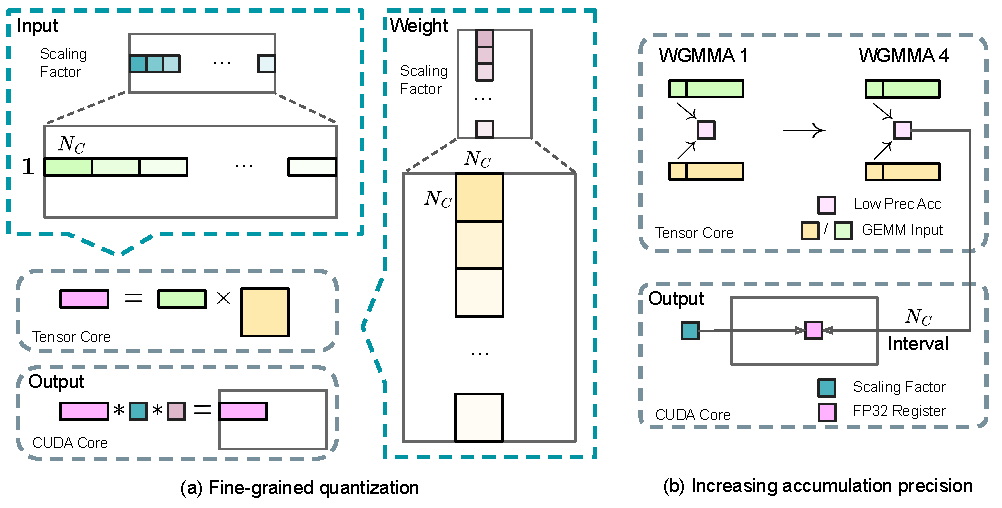
\includegraphics[width=0.95\linewidth]{figures/fp8-128accumulatorv4.pdf}
\caption{
    (a) 我们提出一种细粒度量化方法，以缓解特征离群值导致的量化误差；为简化说明，图中仅展示 \texttt{Fprop}。
    (b) 结合我们的量化策略，我们每隔 $N_C=128$ 个元素 MMA 将结果提升到 CUDA Cores 上进行高精度累加，从而提高 FP8 GEMM 精度。
}
\label{fig:fp8_quantization}
\end{figure}

\subsubsection{通过量化与乘法提升精度}
基于我们的混合精度 FP8 框架，我们引入若干策略来提高低精度训练精度，重点覆盖量化方法和乘法过程。

\paragraph{细粒度量化。}
在低精度训练框架中，由于 FP8 格式的动态范围有限，且受较少指数位约束，溢出和下溢是常见挑战。
标准做法是将输入张量的最大绝对值缩放到 FP8 的最大可表示值，从而使输入分布对齐到 FP8 格式的可表示范围~\citep{fp16train}。
这种方法使低精度训练对激活离群值高度敏感，从而严重降低量化精度。
为解决这一问题，我们提出一种细粒度量化方法，在更细粒度上应用缩放。
如图~\ref{fig:fp8_quantization} (a) 所示，(1) 对激活，我们按 \texttt{1x128} tile 对元素分组并缩放，即每个 token 每 128 个通道；(2) 对权重，我们按 \texttt{128x128} block 对元素分组并缩放，即每 128 个输入通道和每 128 个输出通道。
该方法使量化过程能够根据更小的元素组调整 scale，从而更好地适应离群值。
在附录~\ref{app:fp8_blockwise} 中，我们进一步讨论了像权重量化一样按 block 对激活分组和缩放时出现的训练不稳定性。

我们方法中的一项关键修改，是沿 GEMM 操作的内维引入 per-group 缩放因子。
标准 FP8 GEMM 并不直接支持这一功能。
不过，结合我们精确的 FP32 累加策略，它可以得到高效实现。
% We will elaborate it in the following paragraph.

值得注意的是，我们的细粒度量化策略与 microscaling formats 的思想高度一致~\citep{rouhani2023microscaling}，而 NVIDIA 下一代 GPU，Blackwell 系列，的 Tensor Cores 已宣布支持量化粒度更小的 microscaling formats~\citep{nvidia_tensor_cores}。
我们希望该设计能为后续工作提供参考，以跟上最新 GPU 架构的发展。

\paragraph{提高累加精度。}
低精度 GEMM 操作常遭遇下溢问题，其精度很大程度上依赖高精度累加，而高精度累加通常以 FP32 精度执行~\citep{bf16train, fp16train}。
然而，我们观察到 NVIDIA H800 GPU 上 FP8 GEMM 的累加精度仅能保留约 14 bit，显著低于 FP32 累加精度。
当内维 \texttt{K} 较大时，这一问题会更加突出~\citep{switchback}，而在扩大 batch size 和模型宽度的大规模模型训练中，这正是典型场景。
以 \texttt{K} = 4096 的两个随机矩阵 GEMM 操作为例，在我们的初步测试中，Tensor Cores 中有限的累加精度导致最大相对误差接近 2\%。
尽管存在这些问题，有限累加精度仍是一些 FP8 框架的默认选项~\citep{transformerengine}，严重限制了训练精度。

为解决这一问题，我们采用提升到 CUDA Cores 上进行更高精度计算的策略~\citep{Thakkar_CUTLASS_2023}。
该过程如图~\ref{fig:fp8_quantization} (b) 所示。
具体而言，在 Tensor Cores 上执行 MMA，Matrix Multiply-Accumulate，期间，中间结果以有限 bit 宽累加。
一旦达到 $N_C$ 的间隔，这些部分结果就会被复制到 CUDA Cores 上的 FP32 寄存器，并在那里执行全精度 FP32 累加。
如前所述，我们的细粒度量化沿内维 \texttt{K} 应用 per-group 缩放因子。
这些缩放因子可以在 CUDA Cores 上作为反量化过程高效相乘，只带来极小的额外计算成本。

值得注意的是，这一修改会降低单个 warpgroup 的 WGMMA，Warpgroup-level Matrix Multiply-Accumulate，指令发射率。然而，在 H800 架构上，两个 WGMMA 通常可以并发驻留：当一个 warpgroup 执行提升操作时，另一个可以执行 MMA 操作。该设计使两个操作能够重叠，从而保持 Tensor Cores 的高利用率。
基于我们的实验，将 $N_C=128$ 个元素，即 4 个 WGMMA，设为累加间隔，是在不引入显著开销的前提下明显提高精度的最小间隔。

\paragraph{尾数优先于指数。}
不同于以往工作采用的混合 FP8 格式 \citep{transformerengine, fp8lm, hfp8}，即在 \texttt{Fprop} 中使用 \texttt{E4M3}，4-bit 指数和 3-bit 尾数，在 \texttt{Dgrad} 和 \texttt{Wgrad} 中使用 \texttt{E5M2}，5-bit 指数和 2-bit 尾数，我们在所有张量上采用 \texttt{E4M3} 格式以获得更高精度。
我们认为该方法的可行性来自我们的细粒度量化策略，即 tile 和 block-wise 缩放。
通过在更小的元素组上操作，我们的方法在这些分组元素之间有效共享指数位，从而缓解有限动态范围的影响。

\paragraph{在线量化。}
Tensor-wise 量化框架~\citep{transformerengine, fp8lm} 采用延迟量化，它维护此前迭代中最大绝对值的历史记录，用以推断当前值。
为确保 scale 准确并简化框架，我们对每个 \texttt{1x128} 激活 tile 或 \texttt{128x128} 权重 block 在线计算最大绝对值。
基于该值，我们推导缩放因子，并将激活或权重在线量化为 FP8 格式。

\subsubsection{低精度存储与通信}
结合我们的 FP8 训练框架，我们通过将缓存激活和优化器状态压缩为更低精度格式，进一步降低内存消耗和通信开销。

\paragraph{低精度优化器状态。}
我们采用 BF16 数据格式而非 FP32 来跟踪 AdamW~\citep{adamW} 优化器中的一阶和二阶矩，且未观察到性能下降。
不过，master weights，由优化器存储，和梯度，用于 batch size 累积，仍保留为 FP32，以确保整个训练过程的数值稳定性。

\paragraph{低精度激活。}
如图~\ref{fig:fp8_framework} 所示，\texttt{Wgrad} 操作以 FP8 执行。
为降低内存消耗，自然的选择是以 FP8 格式缓存激活，供 \texttt{Linear} 算子的反向传播使用。
不过，为实现低成本高精度训练，我们对若干算子进行了特别处理：
\begin{quote}
\textbf{(1) 注意力算子之后的 \texttt{Linear} 输入。} 这些激活也会用于注意力算子的反向传播，因此对精度敏感。我们专门为这些激活采用定制的 \texttt{E5M6} 数据格式。此外，这些激活会在反向传播中从 \texttt{1x128} 量化 tile 转换为 \texttt{128x1} tile。为避免引入额外量化误差，所有缩放因子均采用 round scaled，即 2 的整数次幂。

\textbf{(2) MoE 中 SwiGLU 算子的输入。} 为进一步降低内存成本，我们缓存 SwiGLU 算子的输入，并在反向传播中重新计算其输出。这些激活也使用我们的细粒度量化方法以 FP8 存储，在内存效率与计算精度之间取得平衡。
\end{quote}

\paragraph{低精度通信。}
通信带宽是 MoE 模型训练中的关键瓶颈。
为缓解这一挑战，我们将 MoE up-projections 之前的激活量化为 FP8，然后应用 \texttt{dispatch} 组件，这与 MoE up-projections 中的 FP8 \texttt{Fprop} 兼容。与注意力算子之后的 \texttt{Linear} 输入类似，该激活的缩放因子为 2 的整数次幂。
类似策略也应用于 MoE down-projections 之前的激活梯度。
对于前向和反向的 \texttt{combine} 组件，我们均保留 BF16，以维持训练流水线关键部分的训练精度。


\subsection{推理与部署}
\label{sec:inference_deployment}

我们在 H800 集群上部署 \dsviii{}，其中每个节点内的 GPU 使用 NVLink 互连，集群中所有 GPU 通过 IB 完全互连。
为同时保证在线服务的 Service-Level Objective (SLO) 和高吞吐，我们采用如下部署策略，将 \textit{prefilling} 与 \textit{decoding} 阶段分离。

\subsubsection{预填充}

Prefilling 阶段的最小部署单元由 4 个节点和 32 块 GPU 组成。
\texttt{attention} 部分采用 4-way Tensor Parallelism (TP4) 与 Sequence Parallelism (SP)，并结合 8-way Data Parallelism (DP8)。
其较小的 TP size 4 限制了 TP 通信开销。
对于 \texttt{MoE} 部分，我们使用 32-way Expert Parallelism (EP32)，以确保每个专家处理足够大的 batch size，从而提高计算效率。
对于 \texttt{MoE} all-to-all 通信，我们使用与训练相同的方法：首先通过 IB 跨节点传输 token，然后通过 NVLink 在节点内 GPU 之间转发。
特别地，我们对浅层中的 dense MLP 使用 1-way Tensor Parallelism，以节省 TP 通信。

为实现 \texttt{MoE} 部分不同专家之间的负载均衡，我们需要确保每块 GPU 处理的 token 数大致相同。
为此，我们引入 \textit{redundant experts} 部署策略，复制高负载专家并进行冗余部署。
高负载专家基于在线部署期间收集的统计信息检测，并定期调整，例如每 10 分钟一次。
确定冗余专家集合后，我们基于观察到的负载，在节点内 GPU 之间仔细重新排列专家，力求在不增加跨节点 all-to-all 通信开销的情况下，尽可能平衡各 GPU 的负载。
对于 \dsviii{} 的部署，我们在 prefilling 阶段设置 32 个冗余专家。
对于每块 GPU，除其原本承载的 8 个专家外，还会额外承载 1 个冗余专家。

此外，在 prefilling 阶段，为提升吞吐并隐藏 all-to-all 与 TP 通信开销，我们同时处理两个计算负载相近的 micro-batch，将一个 micro-batch 的 \texttt{attention} 和 \texttt{MoE} 与另一个 micro-batch 的 \texttt{dispatch} 和 \texttt{combine} 重叠。

最后，我们正在探索专家的 \textit{dynamic redundancy} 策略，即每块 GPU 承载更多专家，例如 16 个专家，但每个推理 step 只激活 9 个。
在每层的 all-to-all 操作开始前，我们即时计算全局最优路由方案。
考虑到 prefilling 阶段涉及大量计算，计算该路由方案的开销几乎可以忽略。

\subsubsection{解码}

在 decoding 期间，我们将共享专家视为路由专家。
从这一角度看，每个 token 在路由期间会选择 9 个专家，其中共享专家被视为一个总会被选择的重负载专家。
Decoding 阶段的最小部署单元由 40 个节点和 320 块 GPU 组成。
\texttt{attention} 部分采用带 SP 的 TP4，并结合 DP80，而 \texttt{MoE} 部分使用 EP320。
对于 \texttt{MoE} 部分，每块 GPU 仅承载一个专家，另外 64 块 GPU 负责承载冗余专家和共享专家。
\texttt{dispatch} 和 \texttt{combine} 部分的 all-to-all 通信通过 IB 上的直接点对点传输执行，以实现低延迟。
此外，我们使用 IBGDA~\citep{nvidia_ibgda} 技术进一步降低延迟并提升通信效率。

与 prefilling 类似，我们基于在线服务中的专家负载统计，以一定间隔周期性确定冗余专家集合。
不过，由于每块 GPU 只承载一个专家，我们无需重新排列专家。
我们也在探索用于 decoding 的 \textit{dynamic redundancy} 策略。
然而，这需要更仔细地优化用于计算全局最优路由方案的算法，并优化其与 \texttt{dispatch} kernel 的融合，以降低开销。

此外，为提升吞吐并隐藏 all-to-all 通信开销，我们也在探索 decoding 阶段同时处理两个计算负载相近的 micro-batch。
不同于 prefilling，\texttt{attention} 在 decoding 阶段占用更大比例的时间。因此，我们将一个 micro-batch 的 \texttt{attention} 与另一个 micro-batch 的 \texttt{dispatch+MoE+combine} 重叠。
在 decoding 阶段，每个专家的 batch size 相对较小，通常在 256 个 token 以内，瓶颈是内存访问而非计算。
由于 \texttt{MoE} 部分只需加载一个专家的参数，内存访问开销很小，因此使用更少 SM 不会显著影响整体性能。
因此，为避免影响 \texttt{attention} 部分的计算速度，我们可以只为 \texttt{dispatch+MoE+combine} 分配少量 SM。

\subsection{硬件设计建议}
\label{fp8_hardware_design}

基于我们对 all-to-all 通信和 FP8 训练方案的实现，我们向 AI 硬件厂商提出以下芯片设计建议。

\subsubsection{通信硬件}

在 \dsviii{} 中，我们实现了计算与通信的重叠，以在计算期间隐藏通信延迟。
相较串行计算和通信，这显著降低了对通信带宽的依赖。
然而，当前通信实现依赖昂贵的 SM，例如我们为此分配了 H800 GPU 可用 132 个 SM 中的 20 个，这会限制计算吞吐。
此外，使用 SM 进行通信会造成显著低效，因为 tensor cores 完全未被利用。

当前，SM 主要为 all-to-all 通信执行以下任务：
\begin{itemize}[topsep=0pt]
    \item 
    在 IB (InfiniBand) 与 NVLink 域之间\textbf{转发数据}，同时从单块 GPU 聚合发往同一节点内多块 GPU 的 IB 流量。
    \item 
    在 RDMA 缓冲区，已注册的 GPU 内存区域，与输入/输出缓冲区之间\textbf{传输数据}。
    \item 
    为 \texttt{all-to-all} \texttt{combine}\textbf{执行 \texttt{reduce} 操作}。
    \item
    在跨 IB 和 NVLink 域向多个专家分块传输数据期间，\textbf{管理细粒度内存布局}。
\end{itemize}

我们期待未来厂商开发硬件，将这些通信任务从宝贵的计算单元 SM 上卸载，作为 GPU 协处理器或类似 NVIDIA SHARP~\cite{nvsharp} 的网络协处理器。
此外，为降低应用编程复杂度，我们希望该硬件从计算单元视角统一 IB，scale-out，和 NVLink，scale-up，网络。
借助这一统一接口，计算单元可以通过基于简单原语提交通信请求，在整个 IB-NVLink 统一域内轻松完成 \texttt{read}、\texttt{write}、\texttt{multicast} 和 \texttt{reduce} 等操作。

\subsubsection{计算硬件}

\paragraph{Tensor Cores 中更高的 FP8 GEMM 累加精度。}
在 NVIDIA Hopper 架构当前的 Tensor Core 实现中，FP8 GEMM 受到累加精度有限的影响。在根据最大指数右移对齐 32 个尾数乘积后，Tensor Core 只使用每个尾数乘积的最高 14 bit 进行加法，并截断超出该范围的 bit。将加法结果累加到寄存器时也使用 14-bit 精度。我们的实现通过在 CUDA core 中以 FP32 精度将 128 次 FP8$\times$FP8 乘法的加法结果累加到寄存器，部分缓解了这一限制。
尽管这有助于实现成功的 FP8 训练，但它只是 Hopper 架构在 FP8 GEMM 累加精度上的硬件不足所导致的一种折中。
未来芯片需要采用更高精度。
%Therefore, we recommend future chips to support \texttt{at} \texttt{least} 14-bit accumulation precision for 32 mantissa products’ parallel addition and FP32 precision for register accumulation in Tensor Cores, to maintain FP8 training accuracy. We also suggest increasing the parallel addition precision towards full-precision FP32 if feasible.

\paragraph{支持 Tile- 和 Block-Wise 量化。}
当前 GPU 仅支持 per-tensor 量化，缺乏对我们 tile- 和 block-wise 量化这类细粒度量化的原生支持。
在当前实现中，当达到 $N_C$ 间隔时，部分结果会从 Tensor Cores 复制到 CUDA cores，乘以缩放因子，并加到 CUDA cores 上的 FP32 寄存器中。
尽管结合我们精确的 FP32 累加策略后，反量化开销得到显著缓解，但 Tensor Cores 与 CUDA cores 之间频繁的数据移动仍限制了计算效率。
因此，我们建议未来芯片通过使 Tensor Cores 能够接收缩放因子并实现带 group scaling 的 MMA，来支持细粒度量化。
这样，整个部分和累加与反量化过程都可以直接在 Tensor Cores 内完成，直到产生最终结果，从而避免频繁的数据移动。

\paragraph{支持在线量化。}
尽管我们的研究已证明在线量化的有效性，当前实现仍难以有效支持在线量化。
在现有流程中，我们需要从 HBM (High Bandwidth Memory) 读取 128 个 BF16 激活值，即前一计算的输出，用于量化；量化后的 FP8 值随后被写回 HBM，之后又为 MMA 再次读取。
为解决这一低效问题，我们建议未来芯片将 FP8 cast 与 TMA (Tensor Memory Accelerator) 访问融合为单个操作，使量化能在激活从全局内存传输到共享内存期间完成，从而避免频繁的内存读写。
我们还建议支持 warp-level cast 指令以加速，这也进一步促进 layer normalization 与 FP8 cast 的更好融合。
另一种选择是采用 near-memory computing 方法，将计算逻辑放置在 HBM 附近。
在这种情况下，BF16 元素从 HBM 读入 GPU 时即可直接转换为 FP8，从而将片外内存访问减少约 50\%。

\paragraph{支持转置 GEMM 操作。}
当前架构使矩阵转置与 GEMM 操作的融合较为繁琐。
在我们的工作流中，前向传播期间的激活被量化为 \texttt{1x128} FP8 tile 并存储。
在反向传播期间，矩阵需要被读出、反量化、转置、重新量化为 \texttt{128x1} tile，并存储到 HBM。
为减少内存操作，我们建议未来芯片针对训练和推理都需要的精度，在 MMA 操作前支持从共享内存直接转置读取矩阵。结合 FP8 格式转换与 TMA 访问的融合，这项增强将显著简化量化工作流。

\section{预训练}
\label{sec:pre-training}

\subsection{数据构建}

与 \dsvii{} 相比，我们通过提高数学和编程样本比例来优化预训练语料，同时将多语言覆盖范围扩展到英语和中文之外。
此外，我们改进了数据处理流水线，在保持语料多样性的同时尽量减少冗余。
受 \citet{Ding2024FewerTI} 启发，我们为保持数据完整性实现了文档打包方法，但在训练中未加入跨样本注意力掩码。
最终，\dsviii{} 的训练语料在我们的 tokenizer 下包含 14.8T 个高质量且多样的 token。

在 DeepSeekCoder-V2~\citep{dscodervii} 的训练过程中，我们观察到 Fill-in-Middle~(FIM) 策略不会损害 next-token 预测能力，同时使模型能够基于上下文线索准确预测中间文本。
与 DeepSeekCoder-V2 保持一致，我们也在 \dsviii{} 的预训练中引入 FIM 策略。
具体而言，我们采用 Prefix-Suffix-Middle (PSM) 框架按如下方式组织数据：
\begin{align}
\texttt{<|fim\_begin|>}f_{\text{pre}}\texttt{<|fim\_hole|>}f_{\text{suf}}\texttt{<|fim\_end|>}f_{\text{middle}}\texttt{<|eos\_token|>} . \nonumber
\end{align}
该结构作为预打包过程的一部分在文档级别应用。
FIM 策略以 0.1 的比例应用，并与 PSM 框架保持一致。

\dsviii{} 的 tokenizer 采用 Byte-level BPE~\citep{shibata1999byte}，并扩展到 128K token 的词表。
我们修改了 tokenizer 的 pretokenizer 和训练数据，以优化多语言压缩效率。
此外，与 \dsvii{} 相比，新的 pretokenizer 引入了组合标点和换行的 token。
然而，当模型处理没有终止换行符的多行 prompt 时，尤其是在 few-shot 评估 prompt 中，该技巧可能引入 token boundary bias~\citep{tokenboundary}。
为解决这一问题，我们在训练期间随机拆分一定比例的此类组合 token，使模型接触更广泛的特殊情况，并缓解该偏差。

\subsection{超参数}

\paragraph{模型超参数。}
我们将 Transformer 层数设为 61，隐藏维度设为 7168。
所有可学习参数均以标准差 0.006 随机初始化。
在 \dsattn{} 中，我们将注意力头数量 $n_h$ 设为 128，每头维度 $d_h$ 设为 128。
KV 压缩维度 $d_c$ 设为 512，query 压缩维度 $d_c^{\prime}$ 设为 1536。
对于解耦 query 和 key，我们将每头维度 $d_h^R$ 设为 64。
除前三层外，我们用 MoE 层替换所有 FFN。
每个 MoE 层包含 1 个共享专家和 256 个路由专家，其中每个专家的中间隐藏维度为 2048。
在路由专家中，每个 token 会激活 8 个专家，并确保每个 token 最多发送到 4 个节点。
Multi-token prediction 深度 $D$ 设为 1，即除确切的下一个 token 外，每个 token 还会预测一个额外 token。
与 \dsvii{} 一样，\dsviii{} 也在压缩隐向量后使用额外 RMSNorm 层，并在宽度瓶颈处乘以额外缩放因子。
在该配置下，\dsviii{} 总参数量为 671B，其中每个 token 激活 37B 参数。

\paragraph{训练超参数。}
我们使用 AdamW 优化器~\citep{adamW}，超参数设为 $\beta_1=0.9$、$\beta_2=0.95$ 和 $\mathrm{weight\_decay}=0.1$。
预训练期间，我们将最大序列长度设为 4K，并在 14.8T 个 token 上预训练 \dsviii{}。
对于学习率调度，我们首先在前 2K step 中将学习率从 0 线性提升到 $2.2 \times 10^{-4}$。
随后，我们保持 $2.2 \times 10^{-4}$ 的恒定学习率，直到模型消耗 10T 个训练 token。
之后，我们按照余弦衰减曲线，在 4.3T 个 token 内将学习率逐渐衰减到 $2.2 \times 10^{-5}$。
在最后 500B 个 token 的训练期间，我们在前 333B 个 token 中保持 $2.2 \times 10^{-5}$ 的恒定学习率，并在剩余 167B 个 token 中切换到另一个恒定学习率 $7.3 \times 10^{-6}$。
梯度裁剪范数设为 1.0。
我们采用 batch size 调度策略，在前 469B 个 token 的训练中将 batch size 从 3072 逐渐增至 15360，并在剩余训练中保持 15360。
我们使用 pipeline parallelism 将模型的不同层部署在不同 GPU 上；对于每一层，路由专家会均匀部署在属于 8 个节点的 64 块 GPU 上。
对于 node-limited routing，每个 token 最多会被发送到 4 个节点，即 $M=4$。
对于 auxiliary-loss-free 负载均衡，我们将偏置更新速度 $\gamma$ 在前 14.3T 个 token 中设为 0.001，在剩余 500B 个 token 中设为 0.0。
对于平衡损失，我们将 $\alpha$ 设为 0.0001，仅用于避免任意单个序列内出现极端不均衡。
MTP 损失权重 $\lambda$ 在前 10T 个 token 中设为 0.3，在剩余 4.8T 个 token 中设为 0.1。

\begin{figure}[ht]
\centering
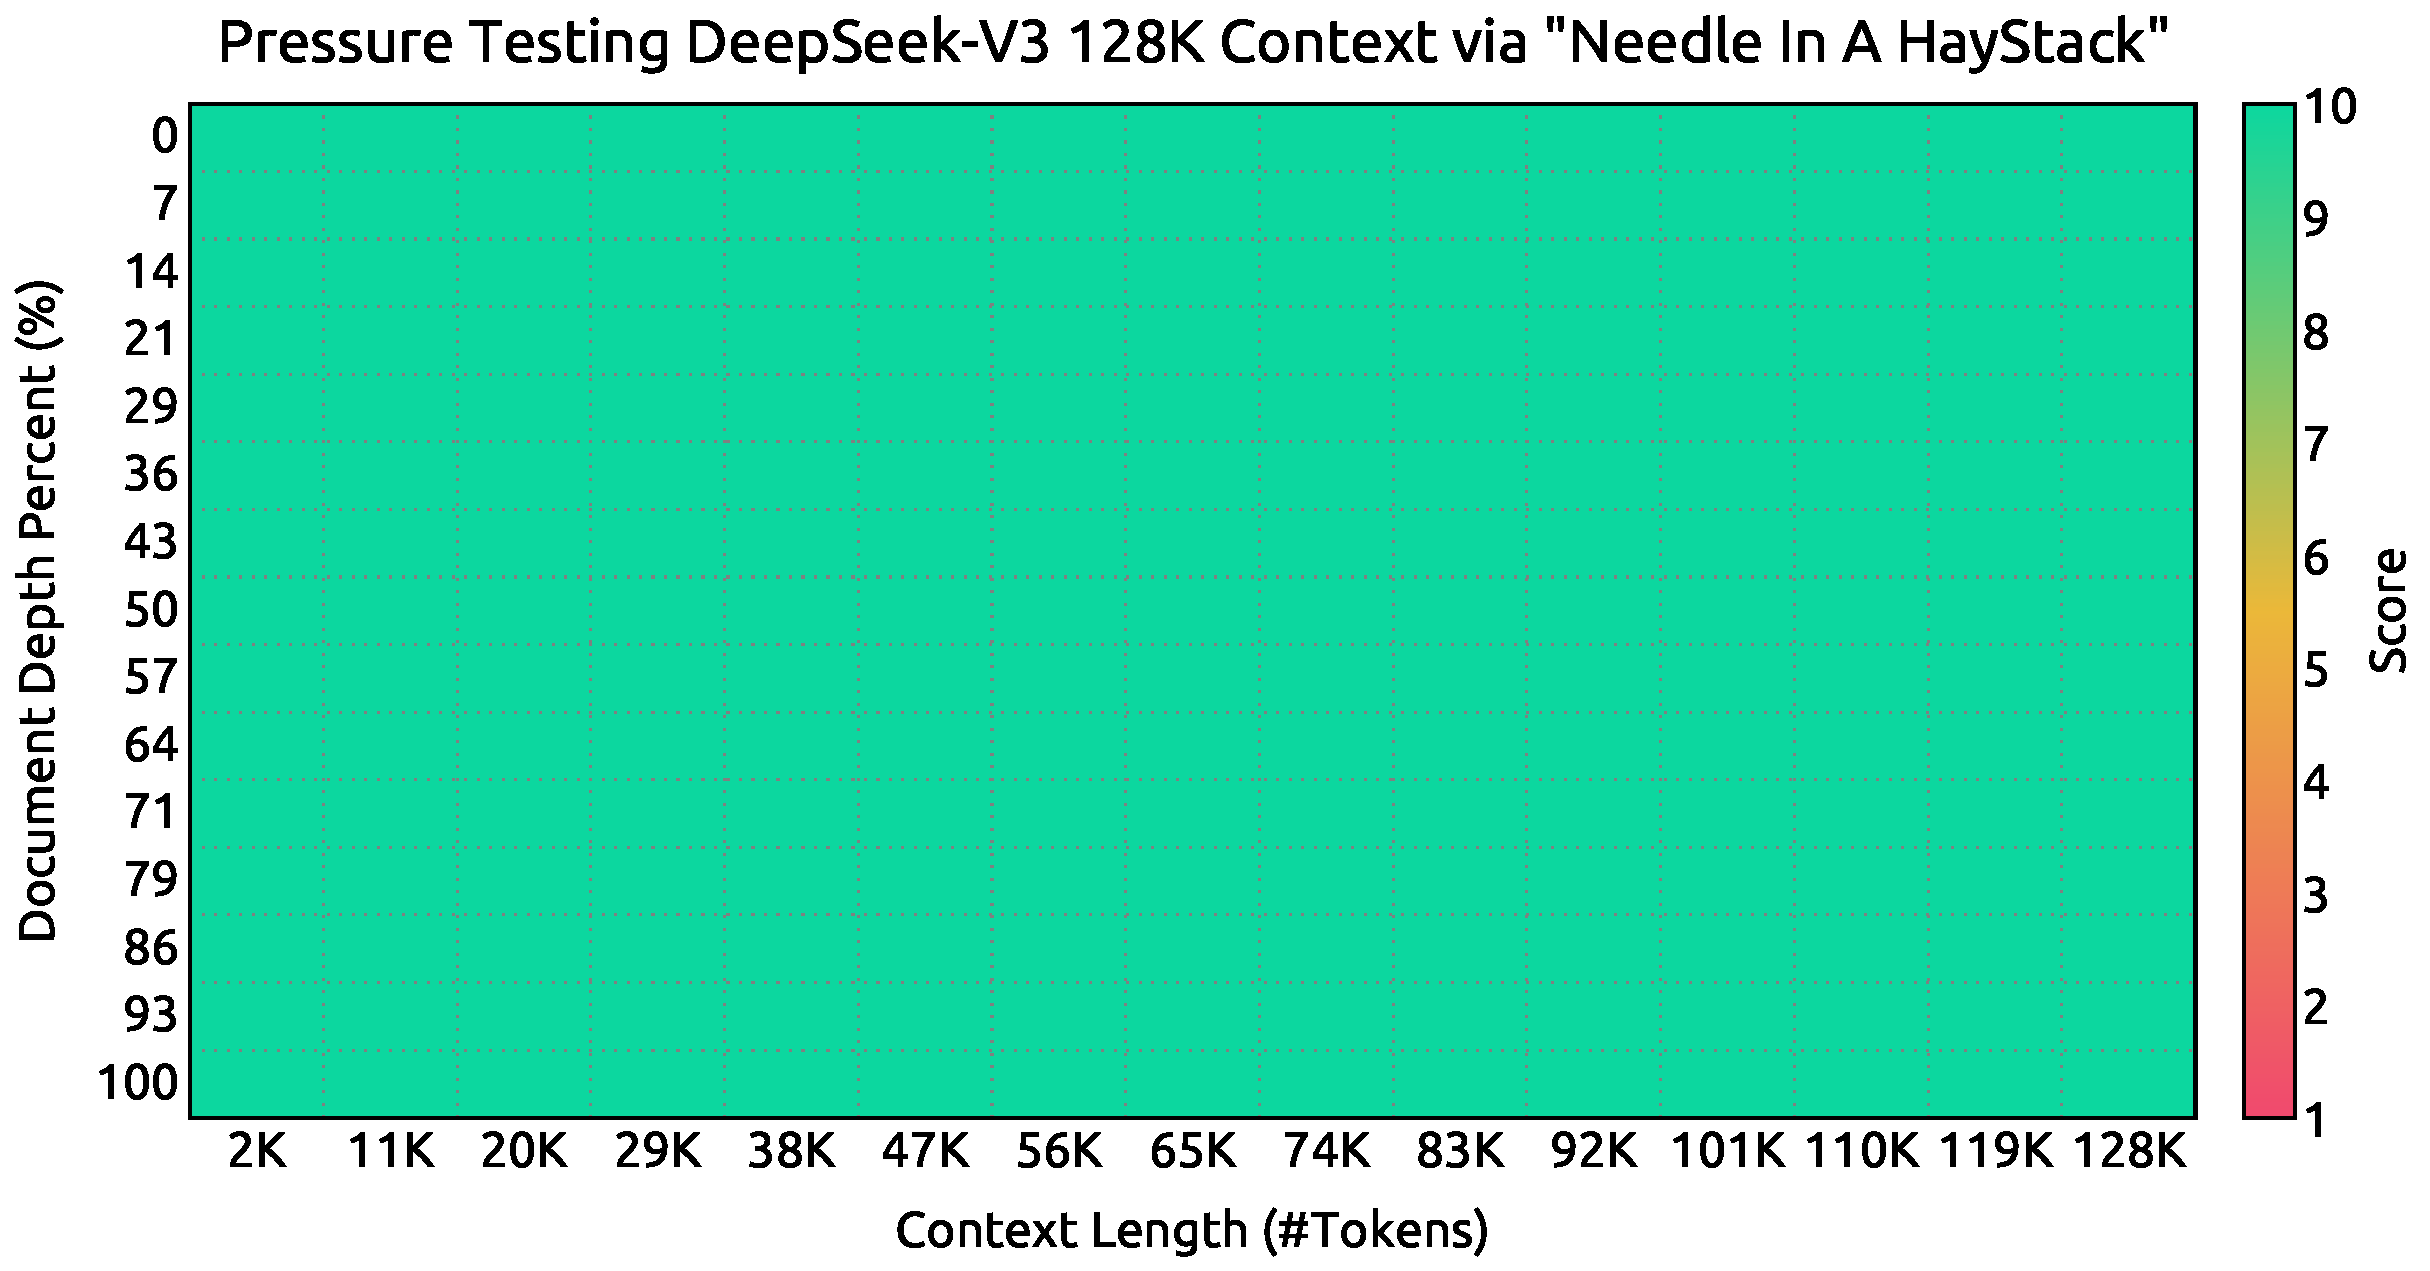
\includegraphics[width=0.98\linewidth]{figures/needle_in_a_haystack.pdf}
\caption{
``Needle In A Haystack'' (NIAH) 测试上的评估结果。
\dsviii{} 在最高 128K 的所有上下文窗口长度上均表现良好。
}
\label{fig:long_context}
\end{figure}

\subsection{长上下文扩展}

我们采用与 \dsvii{}~\citep{dsvii} 类似的方法，使 \dsviii{} 具备长上下文能力。
预训练阶段之后，我们应用 YaRN~\citep{peng2023yarn} 进行上下文扩展，并执行两个额外训练阶段，每个阶段包含 1000 step，将上下文窗口从 4K 逐步扩展到 32K，再扩展到 128K。
YaRN 配置与 \dsvii{} 中使用的配置一致，并且仅应用于解耦共享 key $\mathbf{k}^R_t$。
两个阶段的超参数保持相同，其中 scale $s = 40$，$\alpha = 1$，$\beta = 32$，缩放因子 $\sqrt{t} = 0.1 \ln{s} + 1$。
第一阶段中，序列长度设为 32K，batch size 为 1920。
第二阶段中，序列长度增加到 128K，batch size 降为 480。
两个阶段的学习率均设为 $7.3 \times 10^{-6}$，与预训练阶段的最终学习率一致。

通过这种两阶段扩展训练，\dsviii{} 能够处理长度最高 128K 的输入，同时保持强劲性能。
图~\ref{fig:long_context} 表明，经过 supervised fine-tuning 后，\dsviii{} 在 ``Needle In A Haystack'' (NIAH) 测试上取得显著性能，并在最高 128K 的上下文窗口长度上展现出一致的鲁棒性。

\subsection{评估}

% [list considered benchmarks]
\subsubsection{评估基准}

\dsviii{} 基础模型在以英文和中文为主的多语言语料上预训练，因此我们主要在一系列英文和中文基准以及一个多语言基准上评估其性能。
我们的评估基于集成在 HAI-LLM 框架中的内部评估框架。
所考虑的基准按如下类别列出，其中 \underline{下划线} 基准为中文基准，\uuline{双下划线} 基准为多语言基准：

\textbf{多学科多项选择} 数据集包括 MMLU \citep{mmlu}、MMLU-Redux \citep{mmlu_redux}、MMLU-Pro \citep{mmlu_pro}、\uuline{MMMLU} \citep{mmmlu}、\underline{C-Eval} \citep{ceval} 和 \underline{CMMLU} \citep{cmmlu}。

\textbf{语言理解与推理} 数据集包括 HellaSwag \citep{hellaswag}、PIQA \citep{piqa}、ARC \citep{arc} 和 BigBench Hard (BBH) \citep{bbh}。

\textbf{闭卷问答} 数据集包括 TriviaQA \citep{joshi-etal-2017-triviaqa} 和 NaturalQuestions \citep{naturalquestions}。

\textbf{阅读理解} 数据集包括 RACE \cite{race}、DROP \citep{drop}、\underline{C3} \citep{sun2019investigating} 和 \underline{CMRC} \citep{cui-etal-2019-span}。

\textbf{指代消歧} 数据集包括 \underline{CLUEWSC} \citep{clue} 和 WinoGrande \cite{sakaguchi2019winogrande}。

\textbf{语言建模} 数据集包括 Pile \citep{pile}。

\textbf{中文理解与文化} 数据集包括 \underline{CCPM} \citep{li2021ccpm}。

\textbf{数学} 数据集包括 GSM8K~\citep{gsm8k}、MATH~\citep{hendrycks2021measuring}、MGSM \citep{mgsm} 和 \underline{CMath} \citep{wei2023cmath}。

\textbf{代码} 数据集包括 HumanEval~\citep{codex}、LiveCodeBench-Base (0801-1101) \citep{livecodebench}、MBPP~\citep{mbpp} 和 CRUXEval~\citep{gu2024cruxeval}。

\textbf{标准化考试} 包括 \underline{AGIEval} \citep{agieval}。
需要说明的是，AGIEval 同时包含英文和中文子集。

% [evaluation metrics: ppl, gen, bpb, etc.]
沿袭我们此前的工作~\citep{dsvi,dsvii}，我们对 HellaSwag、PIQA、WinoGrande、RACE-Middle、RACE-High、MMLU、MMLU-Redux、MMLU-Pro、MMMLU、ARC-Easy、ARC-Challenge、C-Eval、CMMLU、C3 和 CCPM 等数据集采用基于困惑度的评估，并对 TriviaQA、NaturalQuestions、DROP、MATH、GSM8K、MGSM、HumanEval、MBPP、LiveCodeBench-Base、CRUXEval、BBH、AGIEval、CLUEWSC、CMRC 和 CMath 采用基于生成的评估。
此外，我们对 Pile-test 执行基于语言建模的评估，并使用 Bits-Per-Byte~(BPB) 作为指标，以保证使用不同 tokenizer 的模型之间公平比较。

\input{tables/base_evaluation}

\subsubsection{评估结果}

在表~\ref{tab:main} 中，我们将 \dsviii{} 基础模型与 state-of-the-art 开源基础模型进行比较，包括 \dsvii{}-Base~\citep{dsvii}，我们的前一版本，Qwen2.5 72B Base~\citep{qwen2_5} 和 LLaMA-3.1 405B Base~\citep{llama3_1_405b}。
我们使用内部评估框架评估所有这些模型，并确保它们采用相同的评估设置。
需要说明的是，由于过去几个月中评估框架发生变化，\dsvii{}-Base 的性能与我们此前报告的结果略有差异。
总体而言，\dsviii{}-Base 全面优于 \dsvii{}-Base 和 Qwen2.5 72B Base，并在多数基准上超过 LLaMA-3.1 405B Base，基本成为最强开源模型。

从更细粒度视角看，我们分别将 \dsviii{}-Base 与其他开源基础模型进行比较。
(1)
相较 \dsvii{}-Base，得益于模型架构改进、模型规模和训练 token 扩大，以及数据质量提升，\dsviii{}-Base 如预期取得显著更好的性能。
(2)
相较 state-of-the-art 中文开源模型 Qwen2.5 72B Base，\dsviii{}-Base 仅使用一半激活参数，却同样展现出显著优势，尤其是在英文、多语言、代码和数学基准上。
至于中文基准，除 CMMLU 这一中文多学科多项选择任务外，\dsviii{}-Base 也展现出优于 Qwen2.5 72B 的性能。
(3)
相较拥有 11 倍激活参数的最大开源模型 LLaMA-3.1 405B Base，\dsviii{}-Base 在多语言、代码和数学基准上也表现得好得多。
对于英文和中文语言基准，\dsviii{}-Base 展现出有竞争力或更好的性能，并且在 BBH、MMLU-series、DROP、C-Eval、CMMLU 和 CCPM 上尤其突出。

得益于高效架构和全面工程优化，\dsviii{} 实现了极高训练效率。
在我们的训练框架和基础设施下，每训练 \dsviii{} 一万亿 token 仅需 180K H800 GPU 小时，远低于训练 72B 或 405B dense 模型的成本。

\begin{table}[ht]
    \centering
    \footnotesize
    \setlength{\tabcolsep}{8pt}
    \begin{tabular}{@{}l c | c c | c c@{}}
    \toprule
    \multirow{2}{*}{\centering \textbf{Benchmark (Metric)}} & \multirow{2}{*}{\textbf{\# Shots}} & \textbf{Small MoE} & \textbf{Small MoE} & \textbf{Large MoE} & \textbf{Large MoE} \\
     & & \textbf{Baseline} & \textbf{w/ MTP} & \textbf{Baseline} & \textbf{w/ MTP} \\
    \midrule
    \# Activated Params {\tiny (Inference)} & - & 2.4B & 2.4B & 20.9B & 20.9B \\
    \# Total Params {\tiny (Inference)} & - & 15.7B & 15.7B & 228.7B & 228.7B \\
    \# Training Tokens & - & 1.33T & 1.33T & 540B & 540B \\
    \midrule
    Pile-test {\tiny (BPB)} & - & \textbf{0.729} & \textbf{0.729} & 0.658 & \textbf{0.657} \\
    BBH {\tiny (EM)} & 3-shot & 39.0 & \textbf{41.4} & 70.0 & \textbf{70.7} \\
    MMLU {\tiny (EM)} & 5-shot & 50.0 & \textbf{53.3} & \textbf{67.5} & 66.6 \\
    DROP {\tiny (F1)} & 1-shot & 39.2 & \textbf{41.3} & 68.5 & \textbf{70.6} \\
    TriviaQA {\tiny (EM)} & 5-shot & 56.9 & \textbf{57.7} & \textbf{67.0} & \textbf{67.3} \\
    NaturalQuestions {\tiny (EM)} & 5-shot & \textbf{22.7} & 22.3 & 27.2 & \textbf{28.5} \\
    HumanEval {\tiny (Pass@1)} & 0-shot & 20.7 & \textbf{26.8} & 44.5 & \textbf{53.7} \\
    MBPP {\tiny (Pass@1)} & 3-shot & 35.8 & \textbf{36.8} & 61.6 & \textbf{62.2} \\
    GSM8K {\tiny (EM)} & 8-shot & 25.4 & \textbf{31.4} & 72.3 & \textbf{74.0} \\
    MATH {\tiny (EM)} & 4-shot & 10.7 & \textbf{12.6} & 38.6 & \textbf{39.8} \\
    \bottomrule
    \end{tabular}
    \caption{
    MTP 策略的消融结果。
    MTP 策略在大多数评估基准上一贯提升模型性能。
    }
    \label{tab:ablation_nextn}
\end{table}

\subsection{讨论}

\subsubsection{Multi-Token Prediction 的消融研究}
\label{discussion:ablation_nextn}

在表~\ref{tab:ablation_nextn} 中，我们展示了 MTP 策略的消融结果。
具体而言，我们在两个不同规模的基线模型上验证 MTP 策略。
在小规模设置中，我们在 1.33T 个 token 上训练一个总参数量为 15.7B 的基线 MoE 模型。
在大规模设置中，我们在 540B 个 token 上训练一个总参数量为 228.7B 的基线 MoE 模型。
在它们之上，我们保持训练数据和其他架构不变，附加一个深度为 1 的 MTP 模块，并训练两个采用 MTP 策略的模型进行比较。
注意，在推理期间，我们直接丢弃 MTP 模块，因此被比较模型的推理成本完全相同。
从表中可以观察到，MTP 策略在大多数评估基准上一贯提升模型性能。

\subsubsection{Auxiliary-Loss-Free 均衡策略的消融研究}
\label{discussion:ablation_noaux_tc}

在表~\ref{tab:ablation_noaux_tc} 中，我们展示了 auxiliary-loss-free 均衡策略的消融结果。
我们在两个不同规模的基线模型上验证该策略。
在小规模设置中，我们在 1.33T 个 token 上训练一个总参数量为 15.7B 的基线 MoE 模型。
在大规模设置中，我们在 578B 个 token 上训练一个总参数量为 228.7B 的基线 MoE 模型。
两个基线模型都仅使用辅助损失鼓励负载均衡，并使用带 top-K 亲和度归一化的 sigmoid gating 函数。
它们用于控制辅助损失强度的超参数分别与 \dsvii{}-Lite 和 \dsvii{} 相同。
在这两个基线模型之上，我们保持训练数据和其他架构不变，移除所有辅助损失并引入 auxiliary-loss-free 均衡策略进行比较。
从表中可以观察到，auxiliary-loss-free 策略在大多数评估基准上一贯取得更好的模型性能。

\begin{table}[t]
    \centering
    \footnotesize
    \setlength{\tabcolsep}{4pt}
    \begin{tabular}{@{}l c | c c | c c@{}}
    \toprule
    \multirow{2}{*}{\centering \textbf{Benchmark (Metric)}} & \multirow{2}{*}{\textbf{\# Shots}} & \textbf{Small MoE} & \textbf{Small MoE} & \textbf{Large MoE} & \textbf{Large MoE} \\
     & & \textbf{Aux-Loss-Based} & \textbf{Aux-Loss-Free} & \textbf{Aux-Loss-Based} & \textbf{Aux-Loss-Free} \\
    \midrule
    \# Activated Params & - & 2.4B & 2.4B & 20.9B & 20.9B \\
    \# Total Params & - & 15.7B & 15.7B & 228.7B & 228.7B \\
    \# Training Tokens & - & 1.33T & 1.33T & 578B & 578B \\
    \midrule
    Pile-test {\tiny (BPB)} & - & 0.727 & \textbf{0.724} & 0.656 & \textbf{0.652} \\
    BBH {\tiny (EM)} & 3-shot & 37.3 & \textbf{39.3} & 66.7 & \textbf{67.9} \\
    MMLU {\tiny (EM)} & 5-shot & 51.0 & \textbf{51.8} & \textbf{68.3} & 67.2 \\
    DROP {\tiny (F1)} & 1-shot & 38.1 & \textbf{39.0} & \textbf{67.1} & \textbf{67.1} \\
    TriviaQA {\tiny (EM)} & 5-shot & \textbf{58.3} & \textbf{58.5} & 66.7 & \textbf{67.7} \\
    NaturalQuestions {\tiny (EM)} & 5-shot & \textbf{23.2} & \textbf{23.4} & 27.1 & \textbf{28.1} \\
    HumanEval {\tiny (Pass@1)} & 0-shot & 22.0 & \textbf{22.6} & 40.2 & \textbf{46.3} \\
    MBPP {\tiny (Pass@1)} & 3-shot & \textbf{36.6} & 35.8 & 59.2 & \textbf{61.2} \\
    GSM8K {\tiny (EM)} & 8-shot & 27.1 & \textbf{29.6} & 70.7 & \textbf{74.5} \\
    MATH {\tiny (EM)} & 4-shot & \textbf{10.9} & \textbf{11.1} & 37.2 & \textbf{39.6} \\
    \bottomrule
    \end{tabular}
    \caption{
    Auxiliary-loss-free 均衡策略的消融结果。
    与纯 auxiliary-loss-based 方法相比，auxiliary-loss-free 策略在大多数评估基准上一贯取得更好的模型性能。
    }
    \label{tab:ablation_noaux_tc}
\end{table}

\subsubsection{Batch-Wise 负载均衡与 Sequence-Wise 负载均衡}
\label{discussion:balance}

Auxiliary-loss-free 均衡与 sequence-wise 辅助损失的关键区别在于均衡范围：batch-wise 与 sequence-wise。
与 sequence-wise 辅助损失相比，batch-wise 均衡施加了更灵活的约束，因为它并不强制每个序列内部保持均衡。
这种灵活性使专家能够更好地专门化于不同领域。
为验证这一点，我们记录并分析了一个 16B auxiliary-loss-based 基线和一个 16B auxiliary-loss-free 模型在 Pile 测试集不同领域上的专家负载。
如图~\ref{fig:expert_load} 所示，我们观察到 auxiliary-loss-free 模型如预期展现出更强的专家专门化模式。

为进一步研究这种灵活性与模型性能优势之间的相关性，我们额外设计并验证了一种 batch-wise 辅助损失，它鼓励每个训练 batch 上的负载均衡，而非每个序列上的负载均衡。
实验结果表明，当达到相似程度的 batch-wise 负载均衡时，batch-wise 辅助损失也能取得与 auxiliary-loss-free 方法相近的模型性能。
具体而言，在我们的 1B MoE 模型实验中，验证损失分别为：2.258，使用 sequence-wise 辅助损失；2.253，使用 auxiliary-loss-free 方法；以及 2.253，使用 batch-wise 辅助损失。
我们在 3B MoE 模型上也观察到类似结果：使用 sequence-wise 辅助损失的模型验证损失为 2.085，而使用 auxiliary-loss-free 方法或 batch-wise 辅助损失的模型验证损失均为 2.080。

此外，尽管 batch-wise 负载均衡方法展现出一致的性能优势，它们也面临两个潜在效率挑战：
(1) 某些序列或小 batch 内的负载不均衡；
(2) 推理期间由 domain-shift 引发的负载不均衡。
第一个挑战由我们的训练框架自然解决，该框架使用大规模 expert parallelism 和 data parallelism，保证每个 micro-batch 具有较大规模。
对于第二个挑战，我们也设计并实现了带冗余专家部署的高效推理框架，如 Section \ref{sec:inference_deployment} 所述，以克服该问题。

\begin{figure}[!t]
\centering
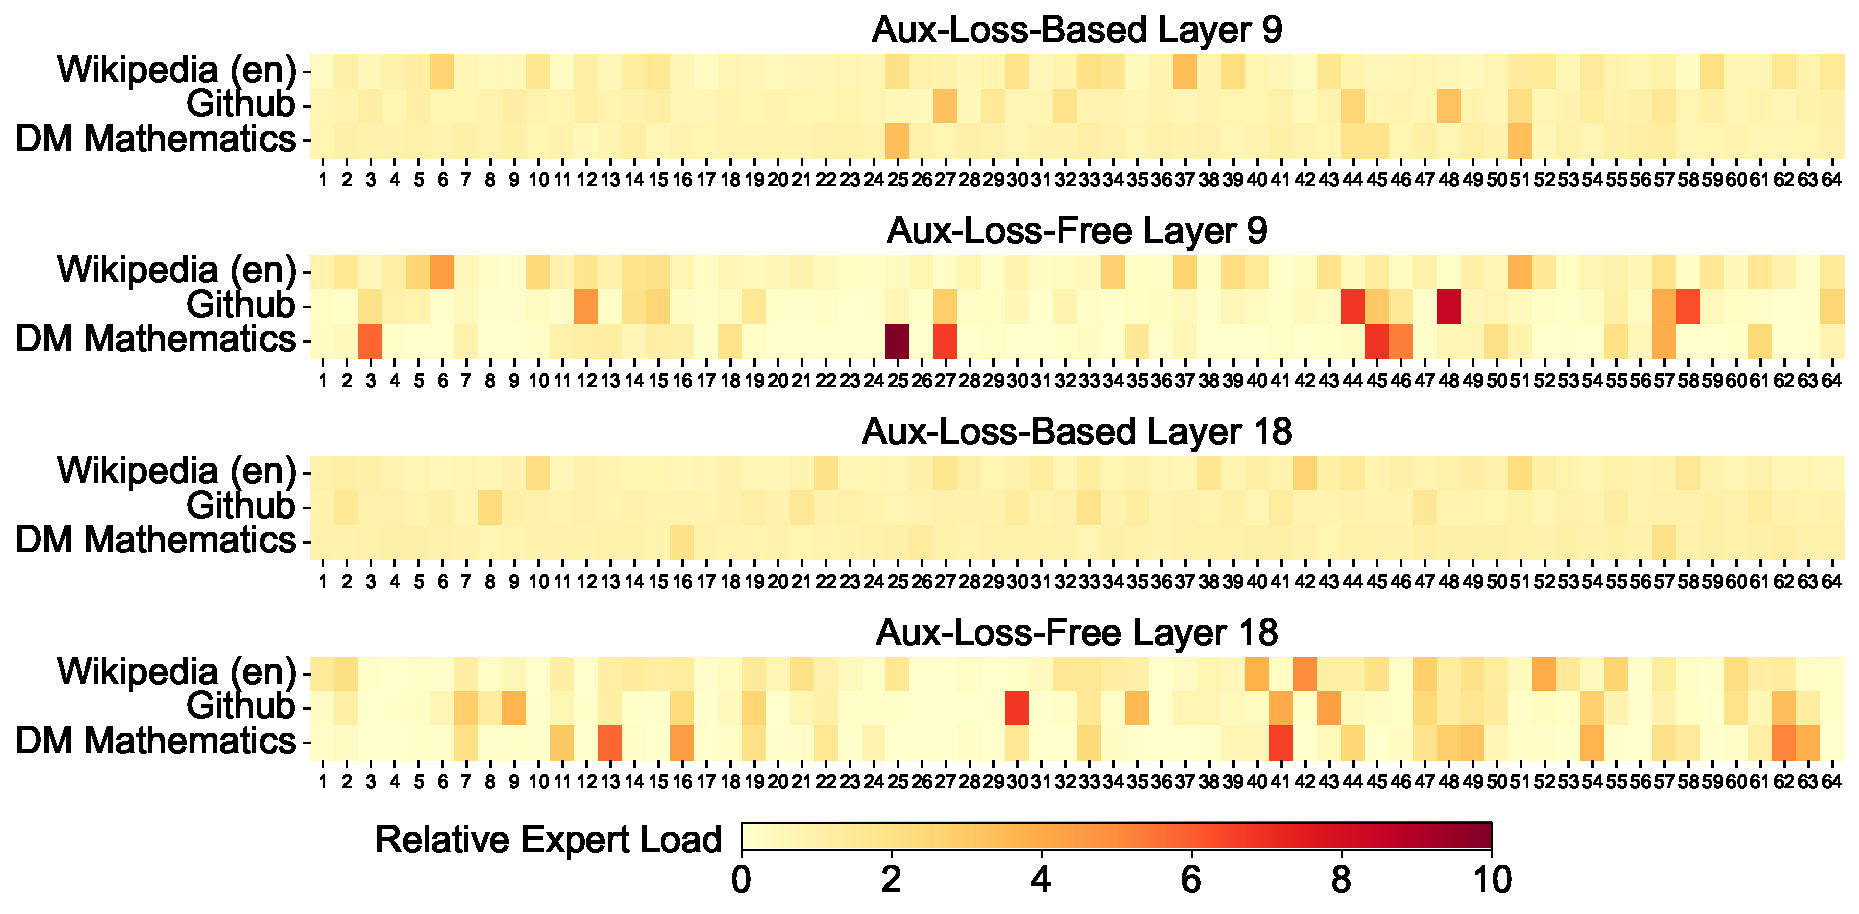
\includegraphics[width=0.99\linewidth]{figures/relative_expert_load_multi.pdf}
\caption{
    Auxiliary-loss-free 和 auxiliary-loss-based 模型在 Pile 测试集三个领域上的专家负载。
    Auxiliary-loss-free 模型比 auxiliary-loss-based 模型展现出更强的专家专门化模式。
    相对专家负载表示实际专家负载与理论均衡专家负载之间的比值。
    由于空间限制，我们仅展示两层结果作为示例，所有层的结果见附录~\ref{app:detailed_expert_load}。
}
\label{fig:expert_load}
\end{figure}

\section{后训练}
\label{sec:alignment}

\subsection{Supervised Fine-Tuning}

我们整理了包含 1.5M 个样本的指令微调数据集，覆盖多个领域，并为每个领域采用契合其特定需求的不同数据创建方法。

\paragraph{推理数据。}
对于推理相关数据集，包括聚焦数学、代码竞赛题和逻辑谜题的数据集，我们使用内部 DeepSeek-R1 模型生成数据。
具体而言，尽管 R1 生成的数据展现出很高准确率，但存在过度思考、格式欠佳和长度过长等问题。
我们的目标是在 R1 生成推理数据的高准确率与常规格式推理数据的清晰简洁之间取得平衡。

为建立我们的方法，我们首先使用结合 Supervised Fine-Tuning (SFT) 与 Reinforcement Learning (RL) 的训练流水线，开发针对特定领域的专家模型，例如代码、数学或通用推理。
该专家模型作为最终模型的数据生成器。
训练过程会为每个样本生成两种不同类型的 SFT 样本：第一种将问题与其原始回答配对，格式为 <problem, original response>；第二种在问题和 R1 回答之外加入 system prompt，格式为 <system prompt, problem, R1 response>。

System prompt 经过精心设计，包含指导模型生成带有反思和验证机制回答的指令。
在 RL 阶段，即便没有显式 system prompt，模型也会利用高 temperature 采样生成融合 R1 生成数据与原始数据模式的回答。
经过数百个 RL step 后，中间 RL 模型学会融入 R1 模式，从而有策略地提升整体性能。

完成 RL 训练阶段后，我们执行 rejection sampling，为最终模型筛选高质量 SFT 数据，其中专家模型被用作数据生成来源。
该方法确保最终训练数据保留 DeepSeek-R1 的优势，同时生成简洁有效的回答。

\paragraph{非推理数据。}
对于非推理数据，例如创意写作、角色扮演和简单问答，我们使用 DeepSeek-V2.5 生成回答，并邀请人工标注员验证数据的准确性和正确性。

\paragraph{SFT 设置。}
我们使用 SFT 数据集对 \dsviii{}-Base 微调两个 epoch，并采用从 $5 \times 10^{-6}$ 开始、逐渐下降到 $1 \times 10^{-6}$ 的余弦衰减学习率调度。
训练期间，每个单独序列由多个样本打包而成。
不过，我们采用样本掩码策略，确保这些样本彼此隔离且相互不可见。

\subsection{强化学习}

\subsubsection{奖励模型}

我们在 RL 过程中使用 rule-based Reward Model (RM) 和 model-based RM。

\paragraph{Rule-Based RM。}
对于可使用特定规则验证的问题，我们采用 rule-based 奖励系统来确定反馈。
例如，某些数学问题具有确定性结果，我们要求模型以指定格式，例如放在方框中，给出最终答案，使我们可以应用规则验证正确性。
类似地，对于 LeetCode 问题，我们可以使用编译器基于测试用例生成反馈。
通过尽可能使用 rule-based 验证，我们确保了更高可靠性，因为这种方法不易被操纵或利用。

\paragraph{Model-Based RM。}
对于具有自由形式 ground-truth 答案的问题，我们依赖 reward model 判断回答是否匹配期望的 ground-truth。
相反，对于没有确定 ground-truth 的问题，例如涉及创意写作的问题，reward model 的任务是基于问题及其对应答案作为输入提供反馈。
Reward model 从 \dsviii{} SFT checkpoints 训练而来。
为增强其可靠性，我们构造偏好数据，不仅提供最终 reward，还包含导向该 reward 的 chain-of-thought。
该方法有助于缓解特定任务中的 reward hacking 风险。

\subsubsection{组相对策略优化}

与 \dsvii{}~\citep{dsvii} 类似，我们采用 Group Relative Policy Optimization~(GRPO)~\citep{deepseekmath}，它省去了通常与 policy model 同规模的 critic model，转而从组内分数估计 baseline。
具体而言，对于每个问题 $q$，GRPO 从旧 policy model $\pi_{\theta_{old}}$ 采样一组输出 $\{o_1, o_2, \cdots, o_G\}$，然后通过最大化以下目标优化 policy model $\pi_{\theta}$：
\begin{equation}
\begin{split}
    \mathcal{J}_{GRPO}(\theta) &= \mathbb{E}{[q \sim P(Q), \{o_i\}_{i=1}^G \sim \pi_{\theta_{old}}(O|q)]}  \\
    & \frac{1}{G}\sum_{i=1}^G \left( \min \left( \frac{\pi_\theta(o_i |q)}{\pi_{\theta_{old}}(o_i |q)} A_i, \text{clip} \left( \frac{\pi_\theta(o_i |q)}{\pi_{\theta_{old}}(o_i |q)}, 1 - \epsilon, 1 + \epsilon \right)  A_i \right) - \beta \mathbb{D}_{KL}\left(\pi_{\theta} || \pi_{ref}\right)\right) ,
\end{split}
\label{eq:GRPO-obj}
\end{equation}
\begin{equation}
    \mathbb{D}_{KL}\left(\pi_{\theta} || \pi_{ref}\right) = \frac{\pi_{ref}(o_i|q)}{\pi_{\theta}(o_i|q)}- \log\frac{\pi_{ref}(o_i|q)}{\pi_{\theta}(o_i|q)} - 1,
\end{equation}
其中 $\epsilon$ 和 $\beta$ 是超参数；
$\pi_{ref}$ 是参考模型；
$A_i$ 是 advantage，由每组内输出对应的 rewards $\{r_1, r_2, \ldots, r_G\}$ 得到：
\begin{equation}
    A_i = \frac{r_i - {\operatorname{mean}(\{r_1, r_2, \cdots, r_G\})}}{{\operatorname{std}(\{r_1, r_2, \cdots, r_G\})}}.
\end{equation}

在 RL 过程中，我们纳入来自多样领域的 prompt，例如代码、数学、写作、角色扮演和问答。
该方法不仅使模型更贴近人类偏好，还提升了基准性能，尤其是在可用 SFT 数据有限的场景中。

\subsection{评估}

\subsubsection{评估设置}

\paragraph{评估基准。}
除用于基础模型测试的基准外，我们进一步在 IFEval~\citep{IFeval}、FRAMES~\citep{frames}、LongBench v2~\citep{bai2024longbench2}、GPQA~\citep{gpqa}、SimpleQA~\citep{simpleqa}、C-SimpleQA~\citep{csimpleqa}、SWE-Bench Verified~\citep{swe_verified}、Aider~\footnote{\url{https://aider.chat}}、LiveCodeBench~\citep{livecodebench}，题目来自 2024 年 8 月至 2024 年 11 月，Codeforces~\footnote{\url{https://codeforces.com}}、Chinese National High School Mathematics Olympiad (CNMO 2024)\footnote{\url{https://www.cms.org.cn/Home/comp/comp/cid/12.html}} 和 American Invitational Mathematics Examination 2024 (AIME 2024)~\citep{AIME2024} 上评估指令模型。

\paragraph{对比基线。}
我们将聊天模型与若干强基线进行全面评估，包括 \dsvii{}-0506、DeepSeek-V2.5-0905、Qwen2.5 72B Instruct、LLaMA-3.1 405B Instruct、Claude-Sonnet-3.5-1022 和 GPT-4o-0513。
对于 \dsvii{} 模型系列，我们选择最具代表性的变体进行比较。
对于闭源模型，评估通过其各自 API 执行。

\paragraph{详细评估配置。}
对于 MMLU、DROP、GPQA 和 SimpleQA 等标准基准，我们采用 simple-evals 框架中的评估 prompt\footnote{\url{https://github.com/openai/simple-evals}}。
我们在 zero-shot 设置下对 MMLU-Redux 使用 Zero-Eval prompt 格式~\citep{Lin_ZeroEval_A_Unified_2024}。
对于其他数据集，我们遵循其原始评估协议，并使用数据集创建者提供的默认 prompt。
对于代码和数学基准，HumanEval-Mul 数据集总共包含 8 种主流编程语言，Python、Java、Cpp、C\#、JavaScript、TypeScript、PHP 和 Bash。
我们使用 CoT 和非 CoT 方法在 LiveCodeBench 上评估模型性能，其中数据收集自 2024 年 8 月至 2024 年 11 月。
Codeforces 数据集使用参赛者百分位进行衡量。
SWE-Bench verified 使用 agentless 框架~\citep{agentless} 评估。
我们使用 ``diff'' 格式评估 Aider 相关基准。
对于数学评估，AIME 和 CNMO 2024 使用 temperature 0.7 进行评估，结果取 16 次运行的平均值，而 MATH-500 使用 greedy decoding。
我们允许所有模型在每个基准上最多输出 8192 个 token。

\input{tables/chat_evaluation}

\subsubsection{标准评估}

表~\ref{tab:chat} 给出了评估结果，表明 \dsviii{} 是性能最佳的开源模型。
此外，它相较 GPT-4o 和 Claude-3.5-Sonnet 等前沿闭源模型也具有竞争力。

\paragraph{英文基准。}
MMLU 是一个广受认可的基准，用于评估大语言模型在多样知识领域和任务上的性能。
\dsviii{} 展现出有竞争力的性能，与 LLaMA-3.1-405B、GPT-4o 和 Claude-Sonnet 3.5 等顶级模型处于同一水平，同时显著优于 Qwen2.5 72B。
此外，\dsviii{} 在更具挑战性的教育知识基准 MMLU-Pro 上表现出色，紧随 Claude-Sonnet 3.5。
在带有修正标签的 MMLU 改进版本 MMLU-Redux 上，\dsviii{} 超过了同类模型。
此外，在博士级评估测试平台 GPQA-Diamond 上，\dsviii{} 取得了显著成绩，仅次于 Claude 3.5 Sonnet，并以较大幅度超过所有其他竞争者。

在 DROP、LongBench v2 和 FRAMES 等长上下文理解基准上，\dsviii{} 继续展现其顶级模型地位。
它在 DROP 的 3-shot 设置中取得了令人印象深刻的 91.6 F1 分数，超过该类别中的所有其他模型。
在 FRAMES 这一要求对 100k token 上下文进行问答的基准上，\dsviii{} 紧随 GPT-4o，同时以显著幅度超过所有其他模型。
这展示了 \dsviii{} 处理超长上下文任务的强大能力。
\dsviii{} 的长上下文能力还通过其在 LongBench v2 上同类最佳的性能得到进一步验证，该数据集在 DeepSeek V3 发布前数周才发布。
在事实知识基准 SimpleQA 上，\dsviii{} 落后于 GPT-4o 和 Claude-Sonnet，主要原因是其设计重点和资源分配。
\dsviii{} 分配了更多训练 token 来学习中文知识，因此在 C-SimpleQA 上取得了出色性能。
在指令遵循基准上，\dsviii{} 显著优于其前身 \dsvii{} 系列，凸显其理解并遵循用户定义格式约束能力的提升。

\paragraph{代码和数学基准。}
编程对 LLM 来说是一项具有挑战且实用的任务，既包括 SWE-Bench-Verified 和 Aider 等面向工程的任务，也包括 HumanEval 和 LiveCodeBench 等算法任务。
在工程任务中，\dsviii{} 落后于 Claude-Sonnet-3.5-1022，但显著优于开源模型。
开源的 \dsviii{} 有望推动代码相关工程任务的进步。
通过开放其强大能力，\dsviii{} 可以推动软件工程和算法开发等领域的创新与改进，使开发者和研究者能够拓展开源模型在编程任务中可达到的边界。
在算法任务中，\dsviii{} 展现出卓越性能，在 HumanEval-Mul 和 LiveCodeBench 等基准上超过所有基线。
这一成功可归因于其先进的知识蒸馏技术，该技术有效增强了其在算法型任务中的代码生成和问题求解能力。

在数学基准上，\dsviii{} 展现出卓越性能，显著超过基线，并为非 o1-like 模型建立了新的 state-of-the-art。
具体而言，在 AIME、MATH-500 和 CNMO 2024 上，\dsviii{} 在绝对分数上比第二好的模型 Qwen2.5 72B 高约 10\%，对于这些高难度基准而言，这是很大的优势。
这一显著能力凸显了来自 DeepSeek-R1 的蒸馏技术的有效性，该技术已被证明对非 o1-like 模型非常有益。

\paragraph{中文基准。}
Qwen 和 DeepSeek 是两个对中文和英文均有强支持的代表性模型系列。
在事实基准 Chinese SimpleQA 上，\dsviii{} 超过 Qwen2.5-72B 16.4 分，尽管 Qwen2.5 在更大的 18T token 语料上训练，比 \dsviii{} 预训练使用的 14.8T token 多 20\%。

在中文教育知识评估代表性基准 C-Eval 和 CLUEWSC (Chinese Winograd Schema Challenge) 上，\dsviii{} 与 Qwen2.5-72B 展现出相近的性能水平，表明两个模型都针对具有挑战性的中文推理和教育任务进行了良好优化。

\begin{table}[t]
    \centering
    \begin{tabular}{c | c c}
    \toprule
    \textbf{Model} & \textbf{Arena-Hard} & \textbf{AlpacaEval 2.0} \\
    \midrule
    DeepSeek-V2.5-0905 & 76.2 & 50.5\\
    Qwen2.5-72B-Instruct & 81.2 & 49.1  \\
    LLaMA-3.1 405B & 69.3 & 40.5\\
    GPT-4o-0513 & 80.4 &  51.1 \\
    Claude-Sonnet-3.5-1022 & 85.2  & 52.0 \\
    DeepSeek-V3 & \textbf{85.5} & \textbf{70.0} \\
    \bottomrule
    \end{tabular}
    \caption{
    英文开放式对话评估。
    对于 AlpacaEval 2.0，我们使用长度控制胜率作为指标。
    }
    \label{tab:open} 
\end{table}

\subsubsection{开放式评估}

除标准基准外，我们还使用 LLM 作为裁判，在开放式生成任务上评估模型，结果见表~\ref{tab:open}。
具体而言，我们遵循 AlpacaEval 2.0~\citep{alpaca2.0} 和 Arena-Hard~\citep{li2024crowdsourced} 的原始配置，它们使用 GPT-4-Turbo-1106 作为裁判进行成对比较。
在 Arena-Hard 上，\dsviii{} 相对基线 GPT-4-0314 取得超过 86\% 的惊人胜率，表现与 Claude-Sonnet-3.5-1022 等顶级模型相当。
这凸显了 \dsviii{} 的强大能力，尤其是在处理复杂 prompt，包括编码和调试任务，方面。
此外，\dsviii{} 成为首个在 Arena-Hard 基准上超过 85\% 的开源模型，实现了突破性里程碑。
这一成就显著弥合了开源与闭源模型之间的性能差距，为开源模型在挑战性领域可达到的水平设立了新标准。

类似地，\dsviii{} 在 AlpacaEval 2.0 上展现出卓越性能，超过闭源和开源模型。
这说明它在写作任务和处理直接问答场景方面具有出色能力。
值得注意的是，它以 20\% 的显著幅度超过 DeepSeek-V2.5-0905，凸显其在处理简单任务上的大幅改进，并展示了这些进展的有效性。

\subsubsection{作为生成式 Reward Model 的 \dsviii{}}

我们将 \dsviii{} 的判断能力与 state-of-the-art 模型，即 GPT-4o 和 Claude-3.5，进行比较。
表~\ref{tab:rewardbench} 给出了这些模型在 RewardBench \citep{lambert2024rewardbench} 上的性能。
\dsviii{} 取得了与 GPT-4o-0806 和 Claude-3.5-Sonnet-1022 最佳版本相当的性能，同时超过其他版本。
此外，\dsviii{} 的判断能力还可以通过投票技术增强。
因此，我们使用 \dsviii{} 结合投票为开放式问题提供自反馈，从而提升对齐过程的有效性和鲁棒性。

\begin{table}[t]
    \centering
    \begin{tabular}{c | c c c c c}
    \toprule
    \textbf{Model} & \textbf{Chat} & \textbf{Chat-Hard} & \textbf{Safety} & \textbf{Reasoning} & \textbf{Average} \\
    \midrule
    GPT-4o-0513 & 96.6 & 70.4 & 86.7 & 84.9 & 84.7\\
    GPT-4o-0806 & 96.1 & 76.1 & 88.1 & 86.6 & 86.7\\
    GPT-4o-1120 & 95.8 & 71.3 & 86.2 & 85.2 & 84.6\\
    \midrule 
    Claude-3.5-sonnet-0620 & 96.4 & 74.0 & 81.6 & 84.7 & 84.2\\
    Claude-3.5-sonnet-1022 & 96.4 & 79.7 & 91.1 & 87.6 & 88.7\\
    \midrule 
    \dsviii{} & 96.9 & 79.8 & 87.0 & 84.3 & 87.0\\
    \dsviii{} (maj@6) & 96.9 & 82.6 & 89.5 & 89.2 & 89.6\\
    \bottomrule
    \end{tabular}
    \caption{GPT-4o、Claude-3.5-sonnet 和 \dsviii{} 在 RewardBench 上的性能。}
    \label{tab:rewardbench} 
\end{table}

\subsection{讨论}

\subsubsection{来自 DeepSeek-R1 的蒸馏}

我们基于 DeepSeek-V2.5 消融来自 DeepSeek-R1 的蒸馏贡献。
基线在短 CoT 数据上训练，而对比模型使用由上述专家 checkpoints 生成的数据。

表~\ref{tab:distill} 展示了蒸馏数据的有效性，在 LiveCodeBench 和 MATH-500 基准上均带来显著提升。
我们的实验揭示了一个有趣的折中：蒸馏带来更好性能，但也显著增加平均回答长度。
为在模型准确率与计算效率之间保持平衡，我们为 \dsviii{} 的蒸馏谨慎选择了最优设置。

我们的研究表明，从推理模型进行知识蒸馏是 post-training 优化的一个有前景方向。
尽管当前工作聚焦于从数学和编码领域蒸馏数据，该方法也展现出在多种任务领域更广泛应用的潜力。
在这些特定领域中展现出的有效性表明，long-CoT 蒸馏对于提升其他需要复杂推理的认知任务中的模型性能可能具有价值。
在不同领域进一步探索该方法仍是未来研究的重要方向。

\begin{table}[t]
    \centering
    \begin{tabular}{c|cc|cc}
    \toprule
    \multirow{2}{*}{\textbf{Model}} & \multicolumn{2}{c}{\textbf{LiveCodeBench-CoT}} & \multicolumn{2}{c}{\textbf{MATH-500}} \\

     & Pass@1 & Length & Pass@1 & Length\\
    \midrule
     DeepSeek-V2.5 Baseline & 31.1 & 718 & 74.6 & 769\\
     DeepSeek-V2.5 +R1 Distill & 37.4 & 783 &83.2& 1510\\
    \bottomrule
    \end{tabular}
    \caption{
    来自 DeepSeek-R1 的蒸馏贡献。
    LiveCodeBench 和 MATH-500 的评估设置与表~\ref{tab:chat} 中相同。
    }
    \label{tab:distill} 
\end{table}

\subsubsection{Self-Rewarding}

Reward 在 RL 中发挥关键作用，引导优化过程。
在可以通过外部工具直接验证的领域，例如某些代码或数学场景，RL 展现出极高效果。
然而，在更一般的场景中，通过硬编码构建反馈机制并不现实。
在 \dsviii{} 的开发过程中，对于这些更广泛的上下文，我们采用 constitutional AI 方法~\citep{bai2022constitutional}，使用 \dsviii{} 自身的投票评估结果作为反馈来源。
该方法产生了显著的对齐效果，显著提升了 \dsviii{} 在主观评估中的性能。
通过整合额外 constitutional 输入，\dsviii{} 可以朝 constitutional 方向优化。
我们认为，将补充信息与作为反馈来源的 LLM 结合起来的这一范式非常重要。
LLM 充当通用处理器，能够将多样场景中的非结构化信息转化为 reward，最终促进 LLM 的自我改进。
除 self-rewarding 外，我们也致力于发现其他通用且可扩展的奖励方法，以持续提升模型在一般场景中的能力。

\subsubsection{Multi-Token Prediction 评估}

\dsviii{} 并非只预测下一个单独 token，而是通过 MTP 技术预测接下来的 2 个 token。
结合 speculative decoding 框架~\citep{speculative_google,speculative_xhm}，它可以显著加快模型的解码速度。
一个自然的问题是额外预测 token 的接受率。
基于我们的评估，在各种生成主题上，第二个 token 预测的接受率介于 85\% 到 90\% 之间，展现出稳定可靠性。
这种高接受率使 \dsviii{} 能够显著提升解码速度，达到 1.8 倍 TPS (Tokens Per Second)。

\section{结论、局限与未来方向}
\label{sec:conclusion}

本文介绍 \dsviii{}，这是一个大型 MoE 语言模型，总参数量为 671B，激活参数量为 37B，在 14.8T 个 token 上训练。
除 \dsattn{} 和 \dsmoe{} 架构外，它还首创用于负载均衡的 auxiliary-loss-free 策略，并设置 multi-token prediction 训练目标以获得更强性能。
得益于 FP8 训练支持和细致工程优化，\dsviii{} 的训练具有很高性价比。
Post-training 也成功从 DeepSeek-R1 系列模型中蒸馏了推理能力。
全面评估表明，DeepSeek-V3 已成为当前最强的开源模型，并取得了可比于 GPT-4o 和 Claude-3.5-Sonnet 等领先闭源模型的性能。
尽管性能强劲，它仍保持了低训练成本。
包括预训练、上下文长度扩展和 post-training 在内，其完整训练仅需 2.788M H800 GPU 小时。

在承认其强性能和高性价比的同时，我们也认识到 \dsviii{} 存在一些局限，尤其是在部署方面。
首先，为确保高效推理，\dsviii{} 推荐的部署单元相对较大，这可能会给小型团队带来负担。
其次，尽管我们的 \dsviii{} 部署策略已实现超过 \dsvii{} 两倍的端到端生成速度，但仍有进一步提升空间。
幸运的是，随着更先进硬件的发展，这些局限有望自然得到解决。

DeepSeek 始终秉持长期主义，坚持开源模型路线，目标是稳步接近 AGI (Artificial General Intelligence) 的终极目标。
未来，我们计划在以下方向上进行战略性研究投入。
\begin{itemize}
    \item 
    我们将持续研究和改进模型架构，目标是进一步提升训练和推理效率，并努力接近对无限上下文长度的高效支持。
    此外，我们将尝试突破 Transformer 的架构局限，从而推进其建模能力边界。
    \item 
    我们将持续迭代训练数据的数量和质量，并探索引入额外训练信号来源，目标是在更全面的维度上推动数据扩展。
    \item 
    我们将持续探索和迭代模型的深度思考能力，目标是通过扩展推理长度和深度来增强其智能和问题求解能力。
    \item 
    我们将探索更全面且多维的模型评估方法，以避免研究过程中倾向于优化固定基准集合，这种倾向可能造成对模型能力的误导性印象，并影响我们的基础评估。
\end{itemize}

\bibliography{main}

\newpage
\appendix

\section*{附录}

\section{贡献与致谢}

\definecolor{damaiblue}{RGB}{0, 0, 100}
\definecolor{damaigreen}{RGB}{0, 100, 0}
\definecolor{damaired}{RGB}{100, 0, 0}

\begin{multicols}{2} % 开始两栏环境
\noindent
\textbf{\color{damaiblue} 研究与工程} \\
\color{damaiblue} Aixin Liu \\
\color{damaiblue} Bing Xue \\
\color{damaiblue} Bingxuan Wang \\
\color{damaiblue} Bochao Wu \\
\color{damaiblue} Chengda Lu \\
\color{damaiblue} Chenggang Zhao \\
\color{damaiblue} Chengqi Deng \\
\color{damaiblue} Chenyu Zhang* \\
\color{damaiblue} Chong Ruan \\
\color{damaiblue} Damai Dai \\
\color{damaiblue} Daya Guo \\
\color{damaiblue} Dejian Yang \\
\color{damaiblue} Deli Chen \\
\color{damaiblue} Erhang Li \\
\color{damaiblue} Fangyun Lin \\
\color{damaiblue} Fucong Dai \\
\color{damaiblue} Fuli Luo* \\
\color{damaiblue} Guangbo Hao \\
\color{damaiblue} Guanting Chen \\
\color{damaiblue} Guowei Li \\
\color{damaiblue} H. Zhang \\
\color{damaiblue} Han Bao* \\
\color{damaiblue} Hanwei Xu \\
\color{damaiblue} Haocheng Wang* \\
\color{damaiblue} Haowei Zhang \\
\color{damaiblue} Honghui Ding \\
\color{damaiblue} Huajian Xin* \\
\color{damaiblue} Huazuo Gao \\
\color{damaiblue} Hui Qu \\
\color{damaiblue} Jianzhong Guo \\
\color{damaiblue} Jiashi Li \\
\color{damaiblue} Jiawei Wang* \\
\color{damaiblue} Jingchang Chen \\
\color{damaiblue} Jingyang Yuan \\
\color{damaiblue} Junjie Qiu \\
\color{damaiblue} Junlong Li \\
\color{damaiblue} Junxiao Song \\
\color{damaiblue} Kai Dong \\
\color{damaiblue} Kai Hu* \\
\color{damaiblue} Kaige Gao \\
\color{damaiblue} Kang Guan \\
\color{damaiblue} Kexin Huang \\
\color{damaiblue} Kuai Yu \\
\color{damaiblue} Lean Wang \\
\color{damaiblue} Lecong Zhang \\
\color{damaiblue} Liang Zhao \\
\color{damaiblue} Litong Wang \\
\color{damaiblue} Liyue Zhang \\
\color{damaiblue} Mingchuan Zhang \\
\color{damaiblue} Minghua Zhang \\
\color{damaiblue} Minghui Tang \\
\color{damaiblue} Panpan Huang \\
\color{damaiblue} Peiyi Wang \\
\color{damaiblue} Qiancheng Wang \\
\color{damaiblue} Qihao Zhu \\
\color{damaiblue} Qinyu Chen \\
\color{damaiblue} Qiushi Du \\
\color{damaiblue} Ruiqi Ge \\
\color{damaiblue} Ruisong Zhang \\
\color{damaiblue} Ruizhe Pan \\
\color{damaiblue} Runji Wang \\
\color{damaiblue} Runxin Xu \\
\color{damaiblue} Ruoyu Zhang \\
\color{damaiblue} Shanghao Lu \\
\color{damaiblue} Shangyan Zhou \\
\color{damaiblue} Shanhuang Chen \\
\color{damaiblue} Shengfeng Ye \\
\color{damaiblue} Shirong Ma \\
\color{damaiblue} Shiyu Wang \\
\color{damaiblue} Shuiping Yu \\
\color{damaiblue} Shunfeng Zhou \\
\color{damaiblue} Shuting Pan \\
\color{damaiblue} Tao Yun \\
\color{damaiblue} Tian Pei \\
\color{damaiblue} Wangding Zeng \\
\color{damaiblue} Wanjia Zhao* \\
\color{damaiblue} Wen Liu \\
\color{damaiblue} Wenfeng Liang \\
\color{damaiblue} Wenjun Gao \\
\color{damaiblue} Wenqin Yu \\
\color{damaiblue} Wentao Zhang \\
\color{damaiblue} Xiao Bi \\
\color{damaiblue} Xiaodong Liu \\
\color{damaiblue} Xiaohan Wang \\
\color{damaiblue} Xiaokang Chen \\
\color{damaiblue} Xiaokang Zhang \\
\color{damaiblue} Xiaotao Nie \\
\color{damaiblue} Xin Cheng \\
\color{damaiblue} Xin Liu \\
\color{damaiblue} Xin Xie \\
\color{damaiblue} Xingchao Liu \\
\color{damaiblue} Xingkai Yu \\
\color{damaiblue} Xinyu Yang \\
\color{damaiblue} Xinyuan Li \\
\color{damaiblue} Xuecheng Su \\
\color{damaiblue} Xuheng Lin \\
\color{damaiblue} Y.K. Li \\
\color{damaiblue} Y.Q. Wang \\
\color{damaiblue} Y.X. Wei \\
\color{damaiblue} Yang Zhang \\
\color{damaiblue} Yanhong Xu \\
\color{damaiblue} Yao Li \\
\color{damaiblue} Yao Zhao \\
\color{damaiblue} Yaofeng Sun \\
\color{damaiblue} Yaohui Wang \\
\color{damaiblue} Yi Yu \\
\color{damaiblue} Yichao Zhang \\
\color{damaiblue} Yifan Shi \\
\color{damaiblue} Yiliang Xiong \\
\color{damaiblue} Ying He \\
\color{damaiblue} Yishi Piao \\
\color{damaiblue} Yisong Wang \\
\color{damaiblue} Yixuan Tan \\
\color{damaiblue} Yiyang Ma* \\
\color{damaiblue} Yiyuan Liu \\
\color{damaiblue} Yongqiang Guo \\
\color{damaiblue} Yu Wu \\
\color{damaiblue} Yuan Ou \\
\color{damaiblue} Yuduan Wang \\
\color{damaiblue} Yue Gong \\
\color{damaiblue} Yuheng Zou \\
\color{damaiblue} Yujia He \\
\color{damaiblue} Yunfan Xiong \\
\color{damaiblue} Yuxiang Luo \\
\color{damaiblue} Yuxiang You \\
\color{damaiblue} Yuxuan Liu \\
\color{damaiblue} Yuyang Zhou \\
\color{damaiblue} Z.F. Wu \\
\color{damaiblue} Z.Z. Ren \\
\color{damaiblue} Zehui Ren \\
\color{damaiblue} Zhangli Sha \\
\color{damaiblue} Zhe Fu \\
\color{damaiblue} Zhean Xu \\
\color{damaiblue} Zhenda Xie \\
\color{damaiblue} Zhengyan Zhang \\
\color{damaiblue} Zhewen Hao \\
\color{damaiblue} Zhibin Gou \\
\color{damaiblue} Zhicheng Ma \\
\color{damaiblue} Zhigang Yan \\
\color{damaiblue} Zhihong Shao \\
\color{damaiblue} Zhiyu Wu \\
\color{damaiblue} Zhuoshu Li \\
\color{damaiblue} Zihui Gu \\
\color{damaiblue} Zijia Zhu \\
\color{damaiblue} Zijun Liu* \\
\color{damaiblue} Zilin Li \\
\color{damaiblue} Ziwei Xie \\
\color{damaiblue} Ziyang Song \\
\color{damaiblue} Ziyi Gao \\
\color{damaiblue} Zizheng Pan \\

\noindent
\textbf{\color{damaigreen} 数据标注} \\
\color{damaigreen} Bei Feng \\
\color{damaigreen} Hui Li \\
\color{damaigreen} J.L. Cai \\
\color{damaigreen} Jiaqi Ni \\
\color{damaigreen} Lei Xu \\
\color{damaigreen} Meng Li \\
\color{damaigreen} Ning Tian \\
\color{damaigreen} R.J. Chen \\
\color{damaigreen} R.L. Jin \\
\color{damaigreen} Ruyi Chen \\
\color{damaigreen} S.S. Li \\
\color{damaigreen} Shuang Zhou \\
\color{damaigreen} Tianyu Sun \\
\color{damaigreen} X.Q. Li \\
\color{damaigreen} Xiangyue Jin \\
\color{damaigreen} Xiaojin Shen \\
\color{damaigreen} Xiaosha Chen \\
\color{damaigreen} Xiaowen Sun \\
\color{damaigreen} Xiaoxiang Wang \\
\color{damaigreen} Xinnan Song \\
\color{damaigreen} Xinyi Zhou \\
\color{damaigreen} Y.X. Zhu \\
\color{damaigreen} Yanhong Xu \\
\color{damaigreen} Yanping Huang \\
\color{damaigreen} Yaohui Li \\
\color{damaigreen} Yi Zheng \\
\color{damaigreen} Yuchen Zhu \\
\color{damaigreen} Yunxian Ma \\
\color{damaigreen} Zhen Huang \\
\color{damaigreen} Zhipeng Xu \\
\color{damaigreen} Zhongyu Zhang \\

\noindent
\textbf{\color{damaired} 商务与合规} \\
\color{damaired} Dongjie Ji \\
\color{damaired} Jian Liang \\
\color{damaired} Jin Chen \\
\color{damaired} Leyi Xia \\
\color{damaired} Miaojun Wang \\
\color{damaired} Mingming Li \\
\color{damaired} Peng Zhang \\
\color{damaired} Shaoqing Wu \\
\color{damaired} Shengfeng Ye \\
\color{damaired} T. Wang \\
\color{damaired} W.L. Xiao \\
\color{damaired} Wei An \\
\color{damaired} Xianzu Wang \\
\color{damaired} Xinxia Shan \\
\color{damaired} Ying Tang \\
\color{damaired} Yukun Zha \\
\color{damaired} Yuting Yan \\
\color{damaired} Zhen Zhang \\

\end{multicols} % 结束两栏环境

在每个角色内，作者按名字的字母顺序列出。
标有 * 的姓名表示已离开我们团队的成员。

\section{低精度训练的消融研究}
\label{app:fp8}

\begin{figure}[!ht]
\centering
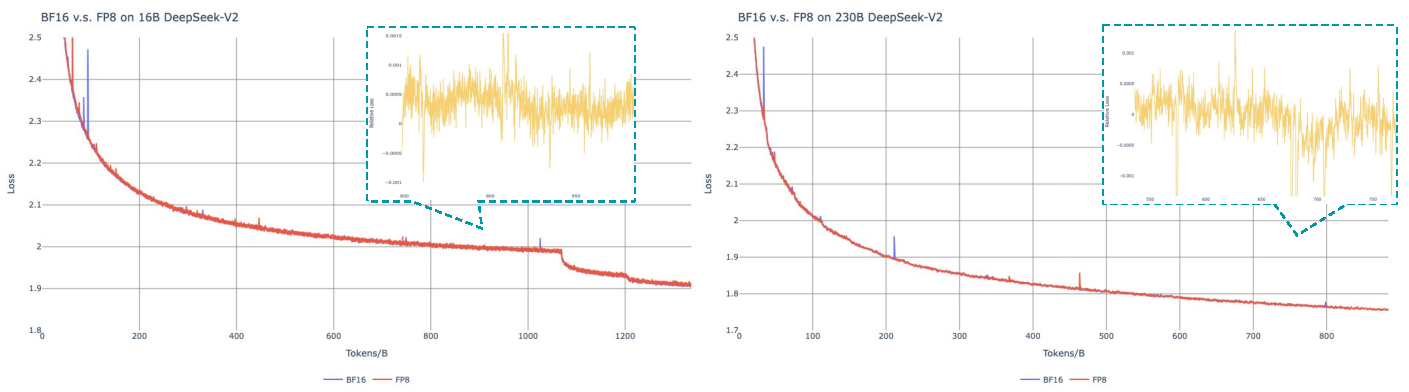
\includegraphics[width=0.95\linewidth]{figures/fp8-v.s.-bf16.pdf}
\caption{
    BF16 与 FP8 训练的损失曲线比较。
    结果使用系数为 0.9 的 Exponential Moving Average (EMA) 进行平滑。
}
\label{fig:fp8_vs_bf16}
\end{figure}

\subsection{FP8 v.s. BF16 训练}
\label{app:fp8_cp_bf16}
我们在两个不同规模的基线模型上，通过与 BF16 训练比较来验证 FP8 混合精度框架。在小规模设置中，我们在 1.33T 个 token 上训练一个总参数量约为 16B 的基线 MoE 模型。
在大规模设置中，我们在约 0.9T 个 token 上训练一个总参数量约为 230B 的基线 MoE 模型。我们在图~\ref{fig:fp8_vs_bf16} 中展示训练曲线，并证明借助我们的高精度累加和细粒度量化策略，相对误差保持在 0.25\% 以下。

\subsection{关于 Block-Wise 量化的讨论}
\label{app:fp8_blockwise}
尽管我们的 tile-wise 细粒度量化有效缓解了特征离群值引入的误差，但它需要为激活量化采用不同分组，即前向传播中的 \texttt{1x128} 和反向传播中的 \texttt{128x1}。
激活梯度也需要类似过程。
一种直接策略是像量化模型权重一样，对每 \texttt{128x128} 个元素应用 block-wise 量化。
这样，反向传播只需转置。
因此，我们进行了一项实验，将所有与 \texttt{Dgrad} 相关的张量按 block-wise 方式量化。
结果表明，\texttt{Dgrad} 操作高度敏感于精度，该操作计算激活梯度并以链式方式反向传播到浅层。
具体而言，对激活梯度进行 block-wise 量化会导致一个总参数量约 16B、训练约 300B token 的 MoE 模型发散。
我们推测，这种敏感性源于激活梯度在 token 之间高度不均衡，从而产生 token-correlated 离群值~\citep{int4train}。
这些离群值无法通过 block-wise 量化方法得到有效处理。

\section{16B Aux-Loss-Based 与 Aux-Loss-Free 模型的专家专门化模式}
\label{app:detailed_expert_load}
我们记录了 16B auxiliary-loss-based 基线和 auxiliary-loss-free 模型在 Pile 测试集上的专家负载。
如图~\ref{fig:detailed_expert_load} 所示，auxiliary-loss-free 模型在所有层上都倾向于具有更强的专家专门化。

\begin{figure}[!t]
    \subfigure[Layers 1-7]{
        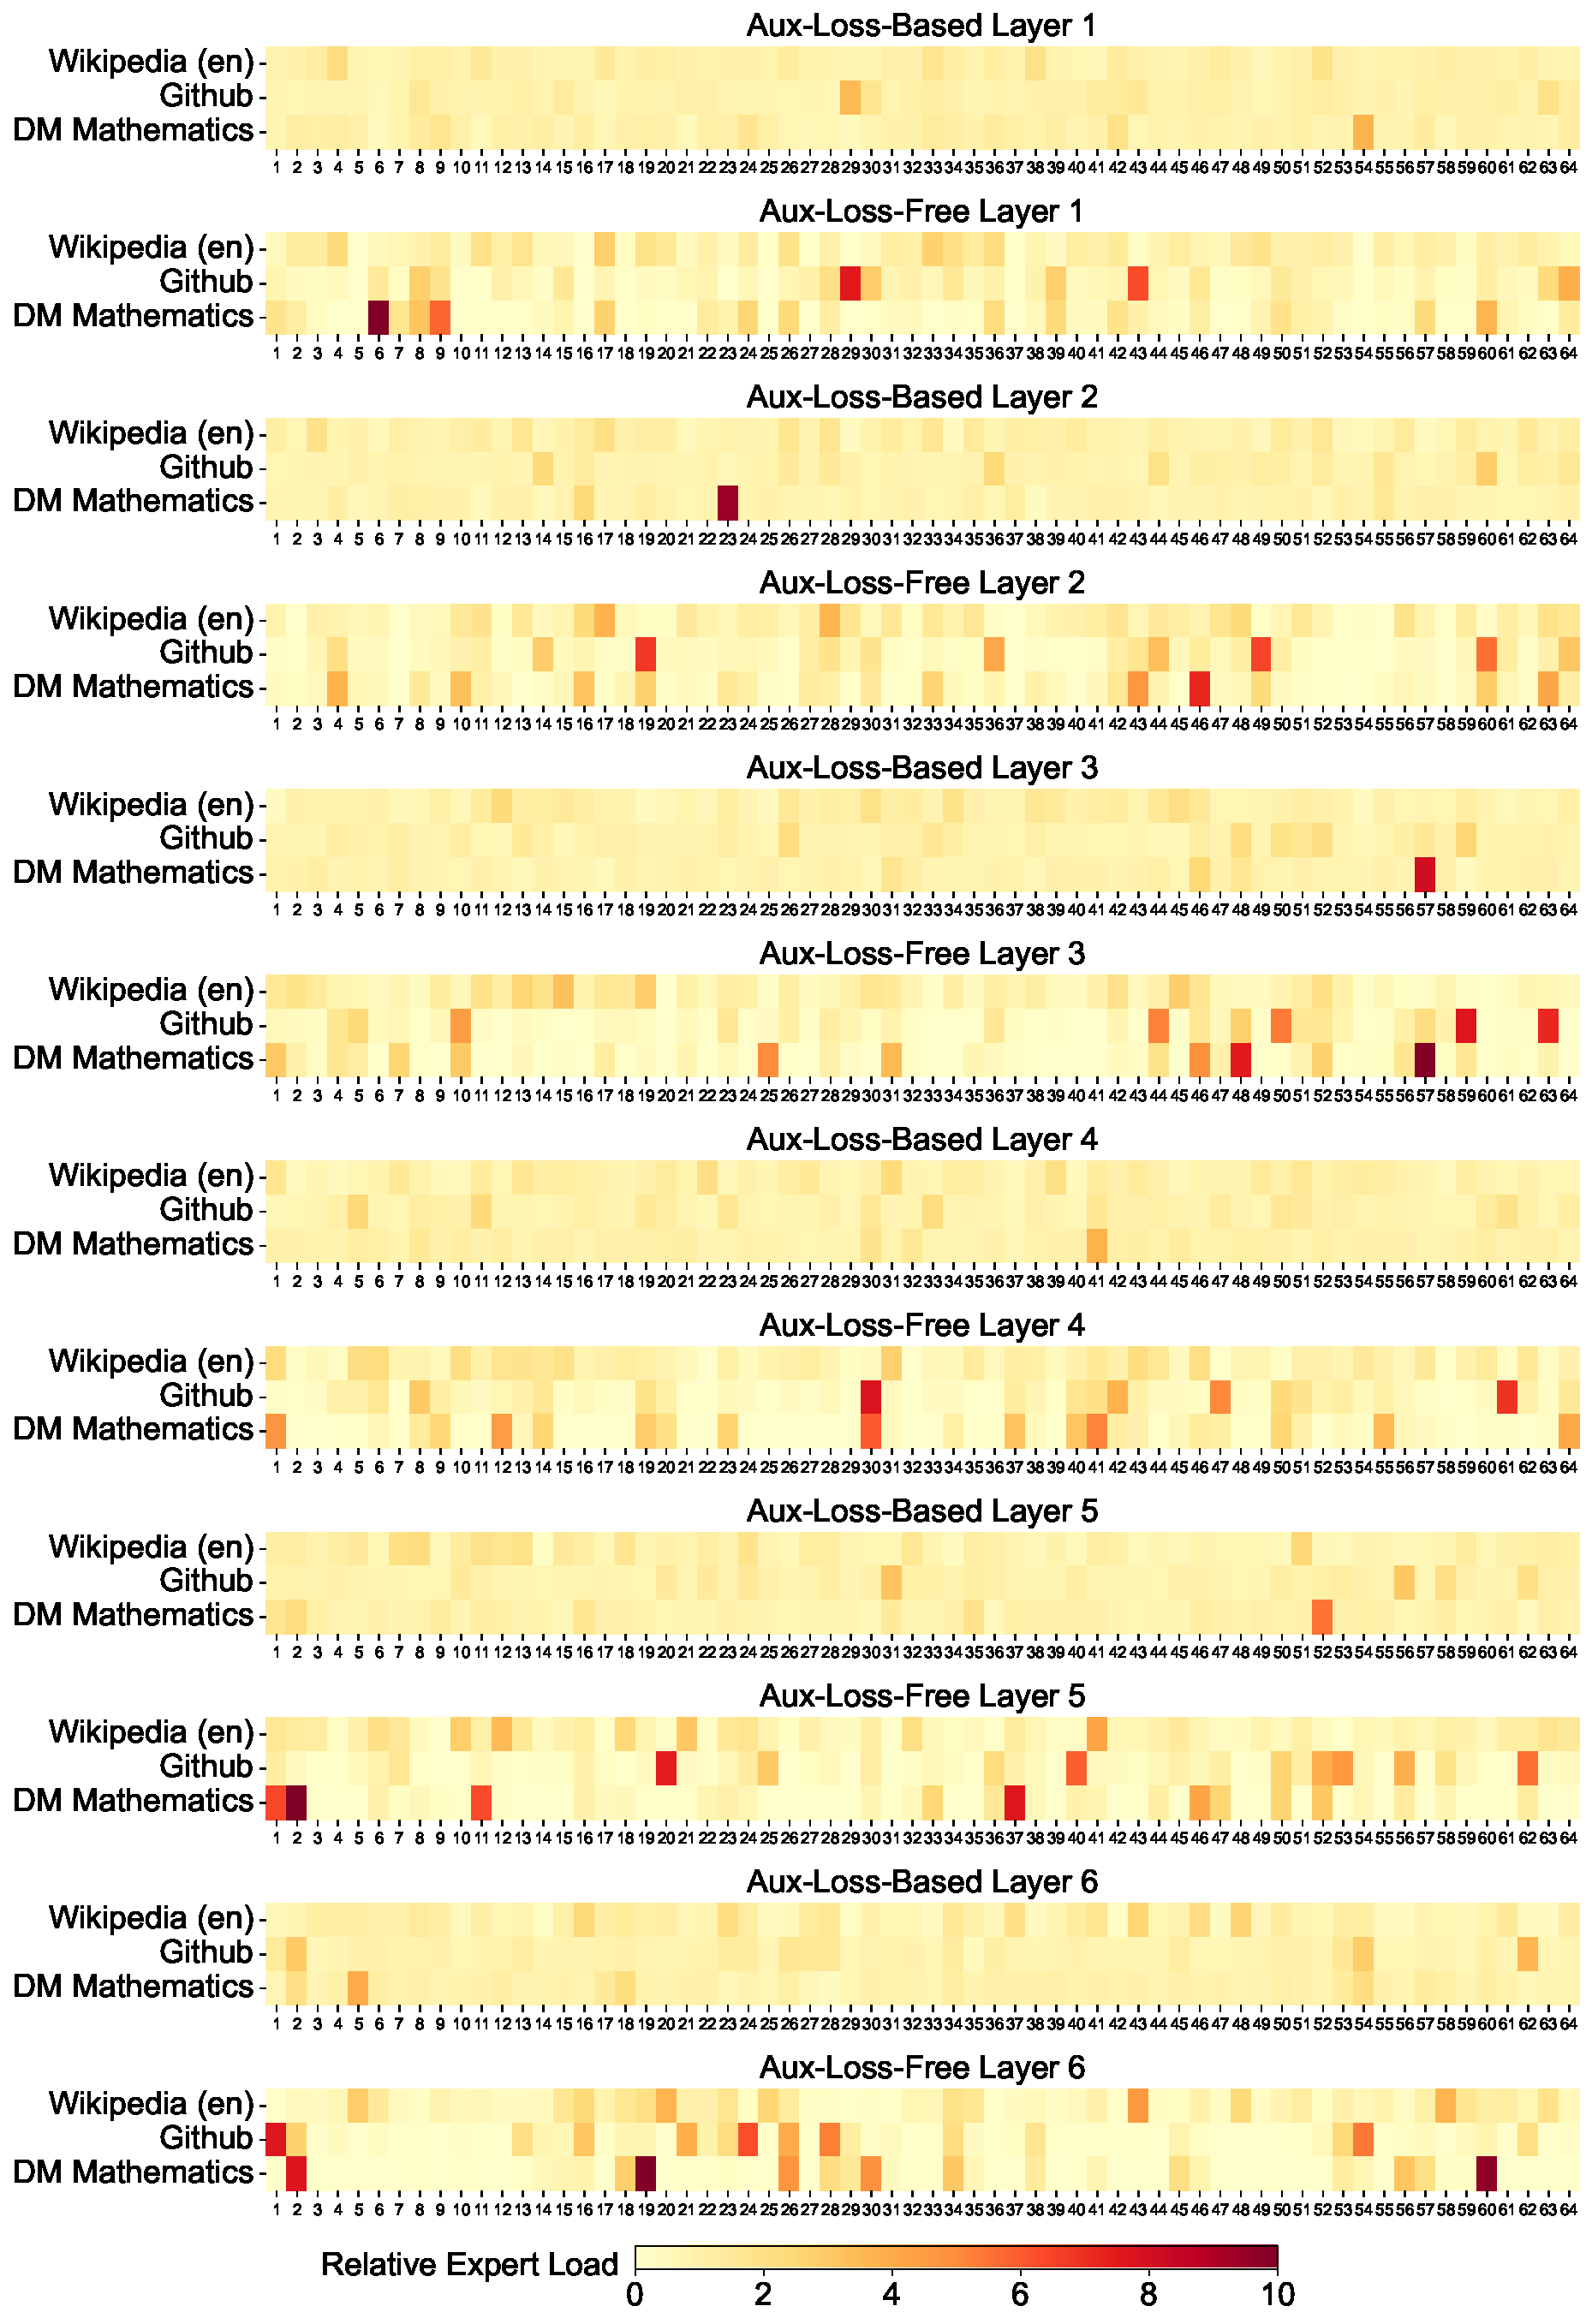
\includegraphics[width=0.95\linewidth]{figures/relative_expert_load_multi_1-6.pdf}
    }
\end{figure}

\begin{figure}[!t]
    \ContinuedFloat
    \subfigure[Layers 7-13]{
        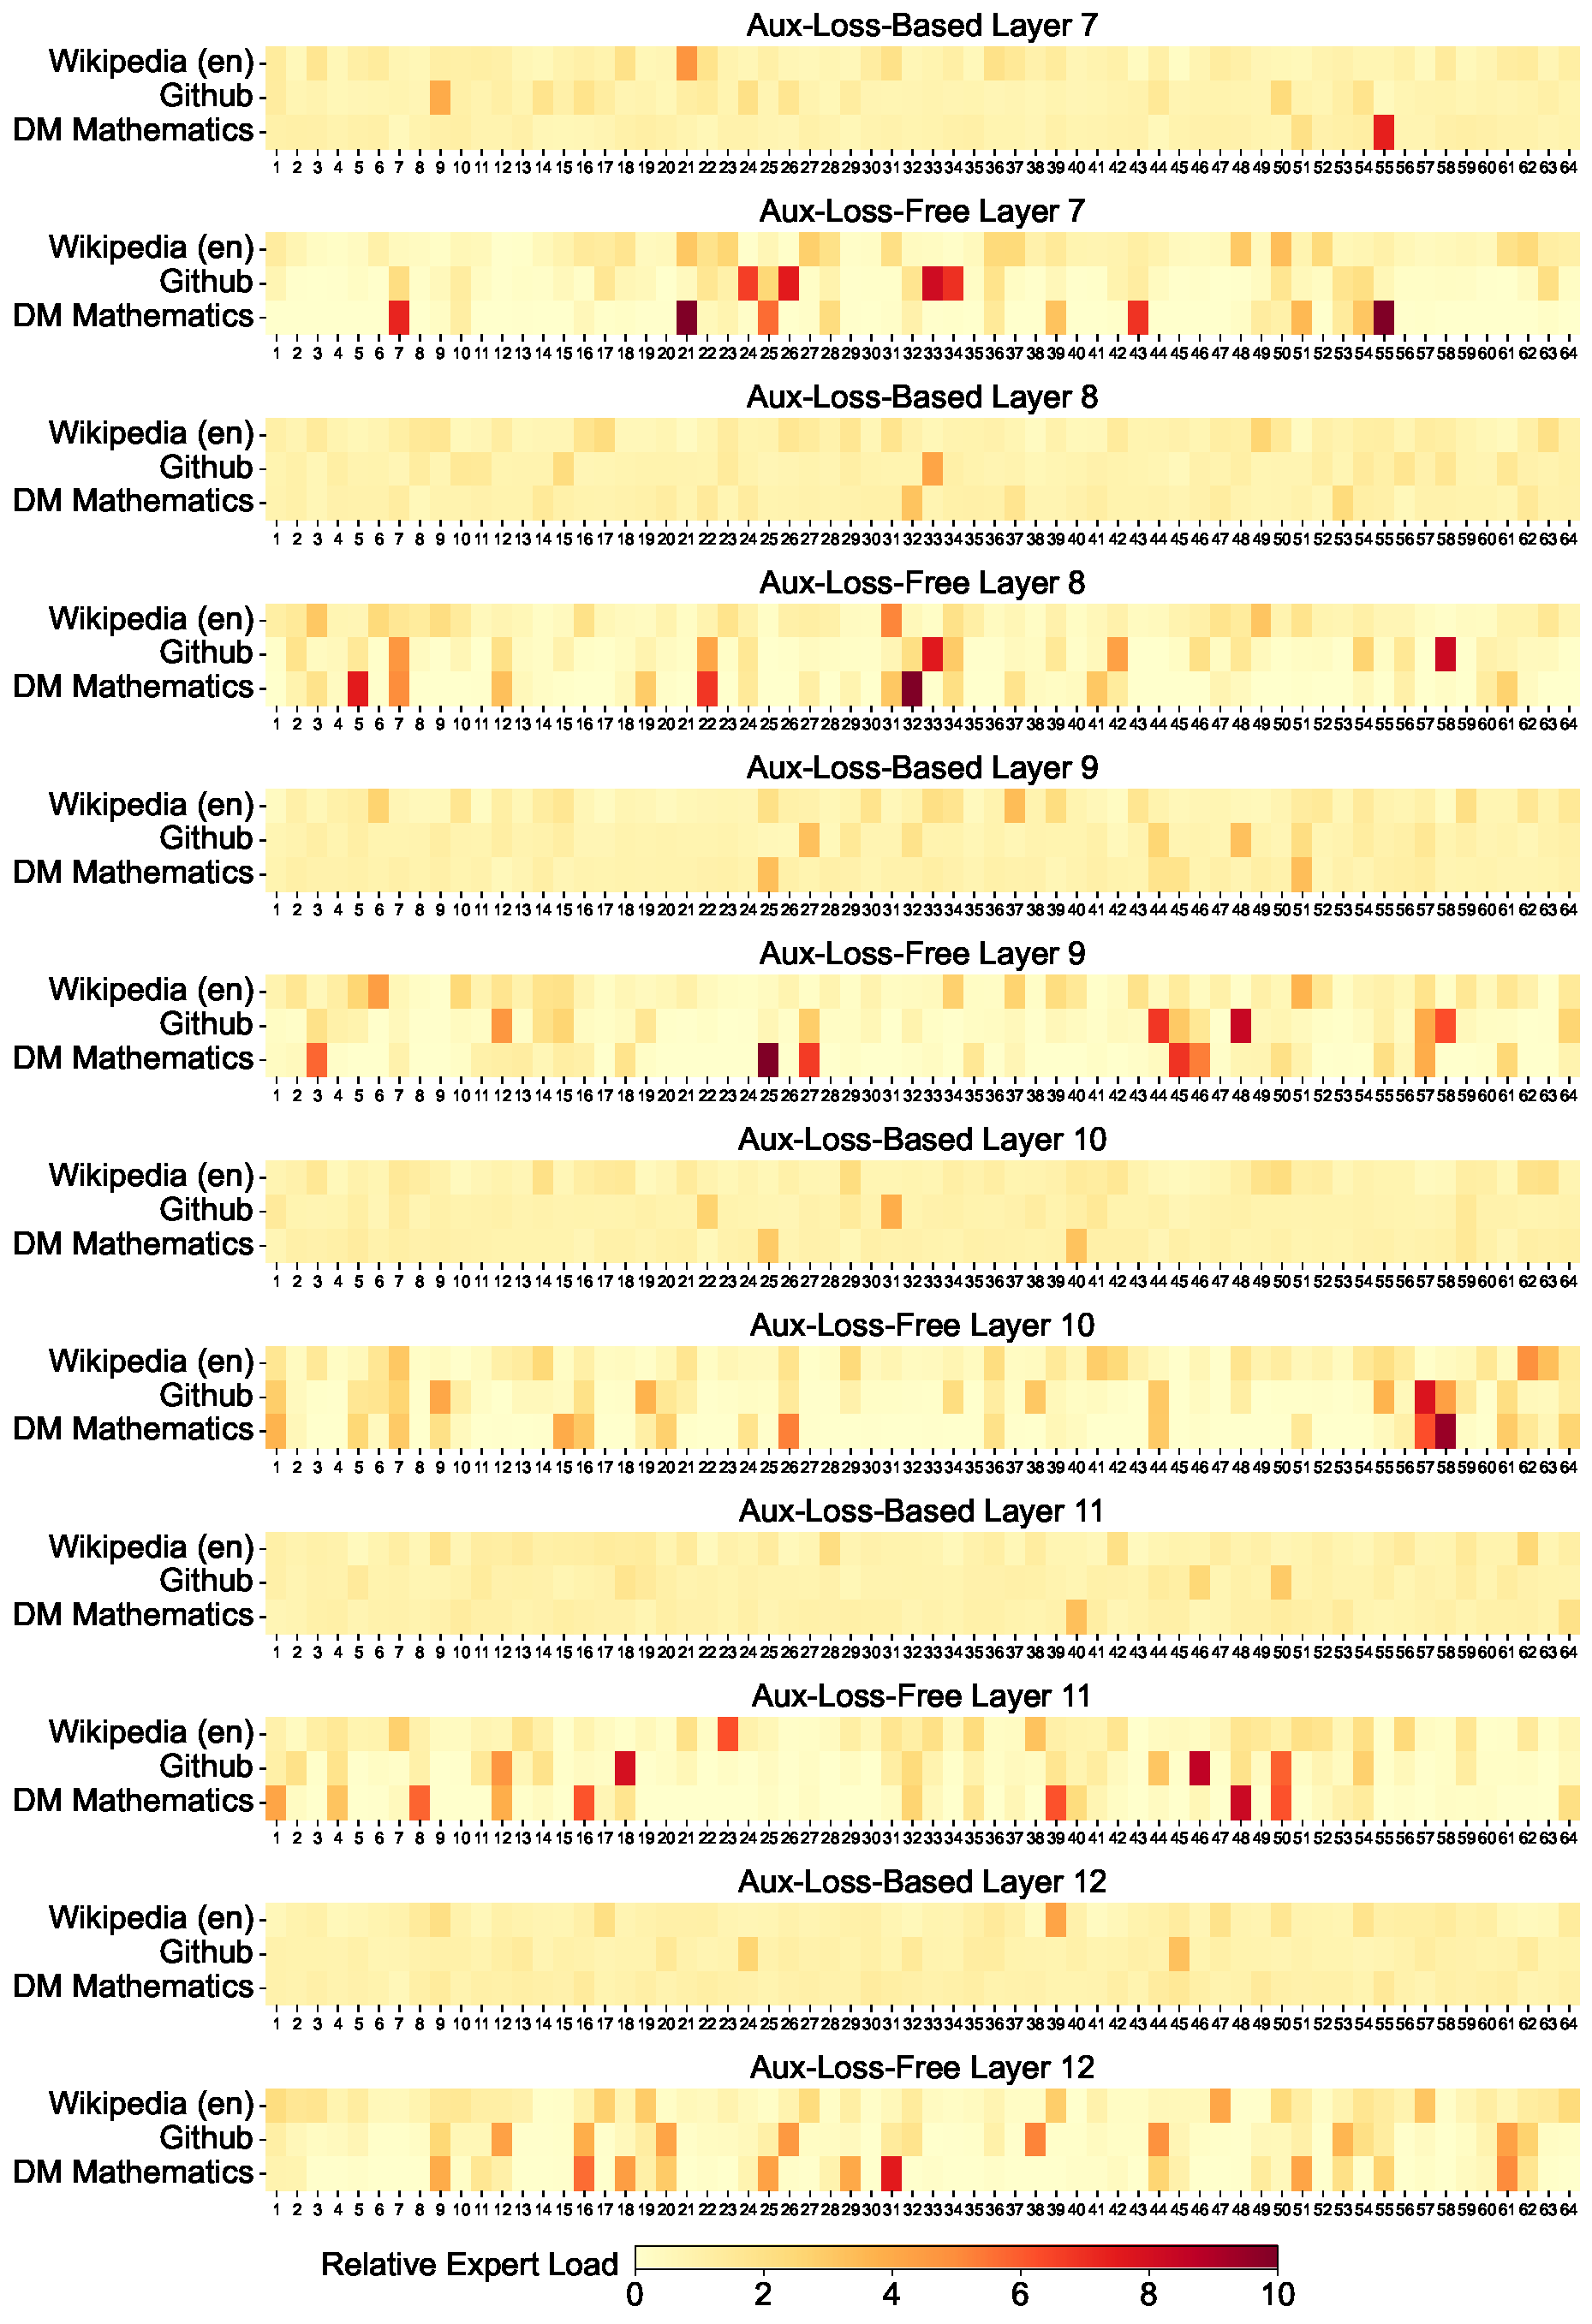
\includegraphics[width=0.95\linewidth]{figures/relative_expert_load_multi_7-12.pdf}
    }
\end{figure}

\begin{figure}[!t]
    \ContinuedFloat
    \subfigure[Layers 13-19]{
        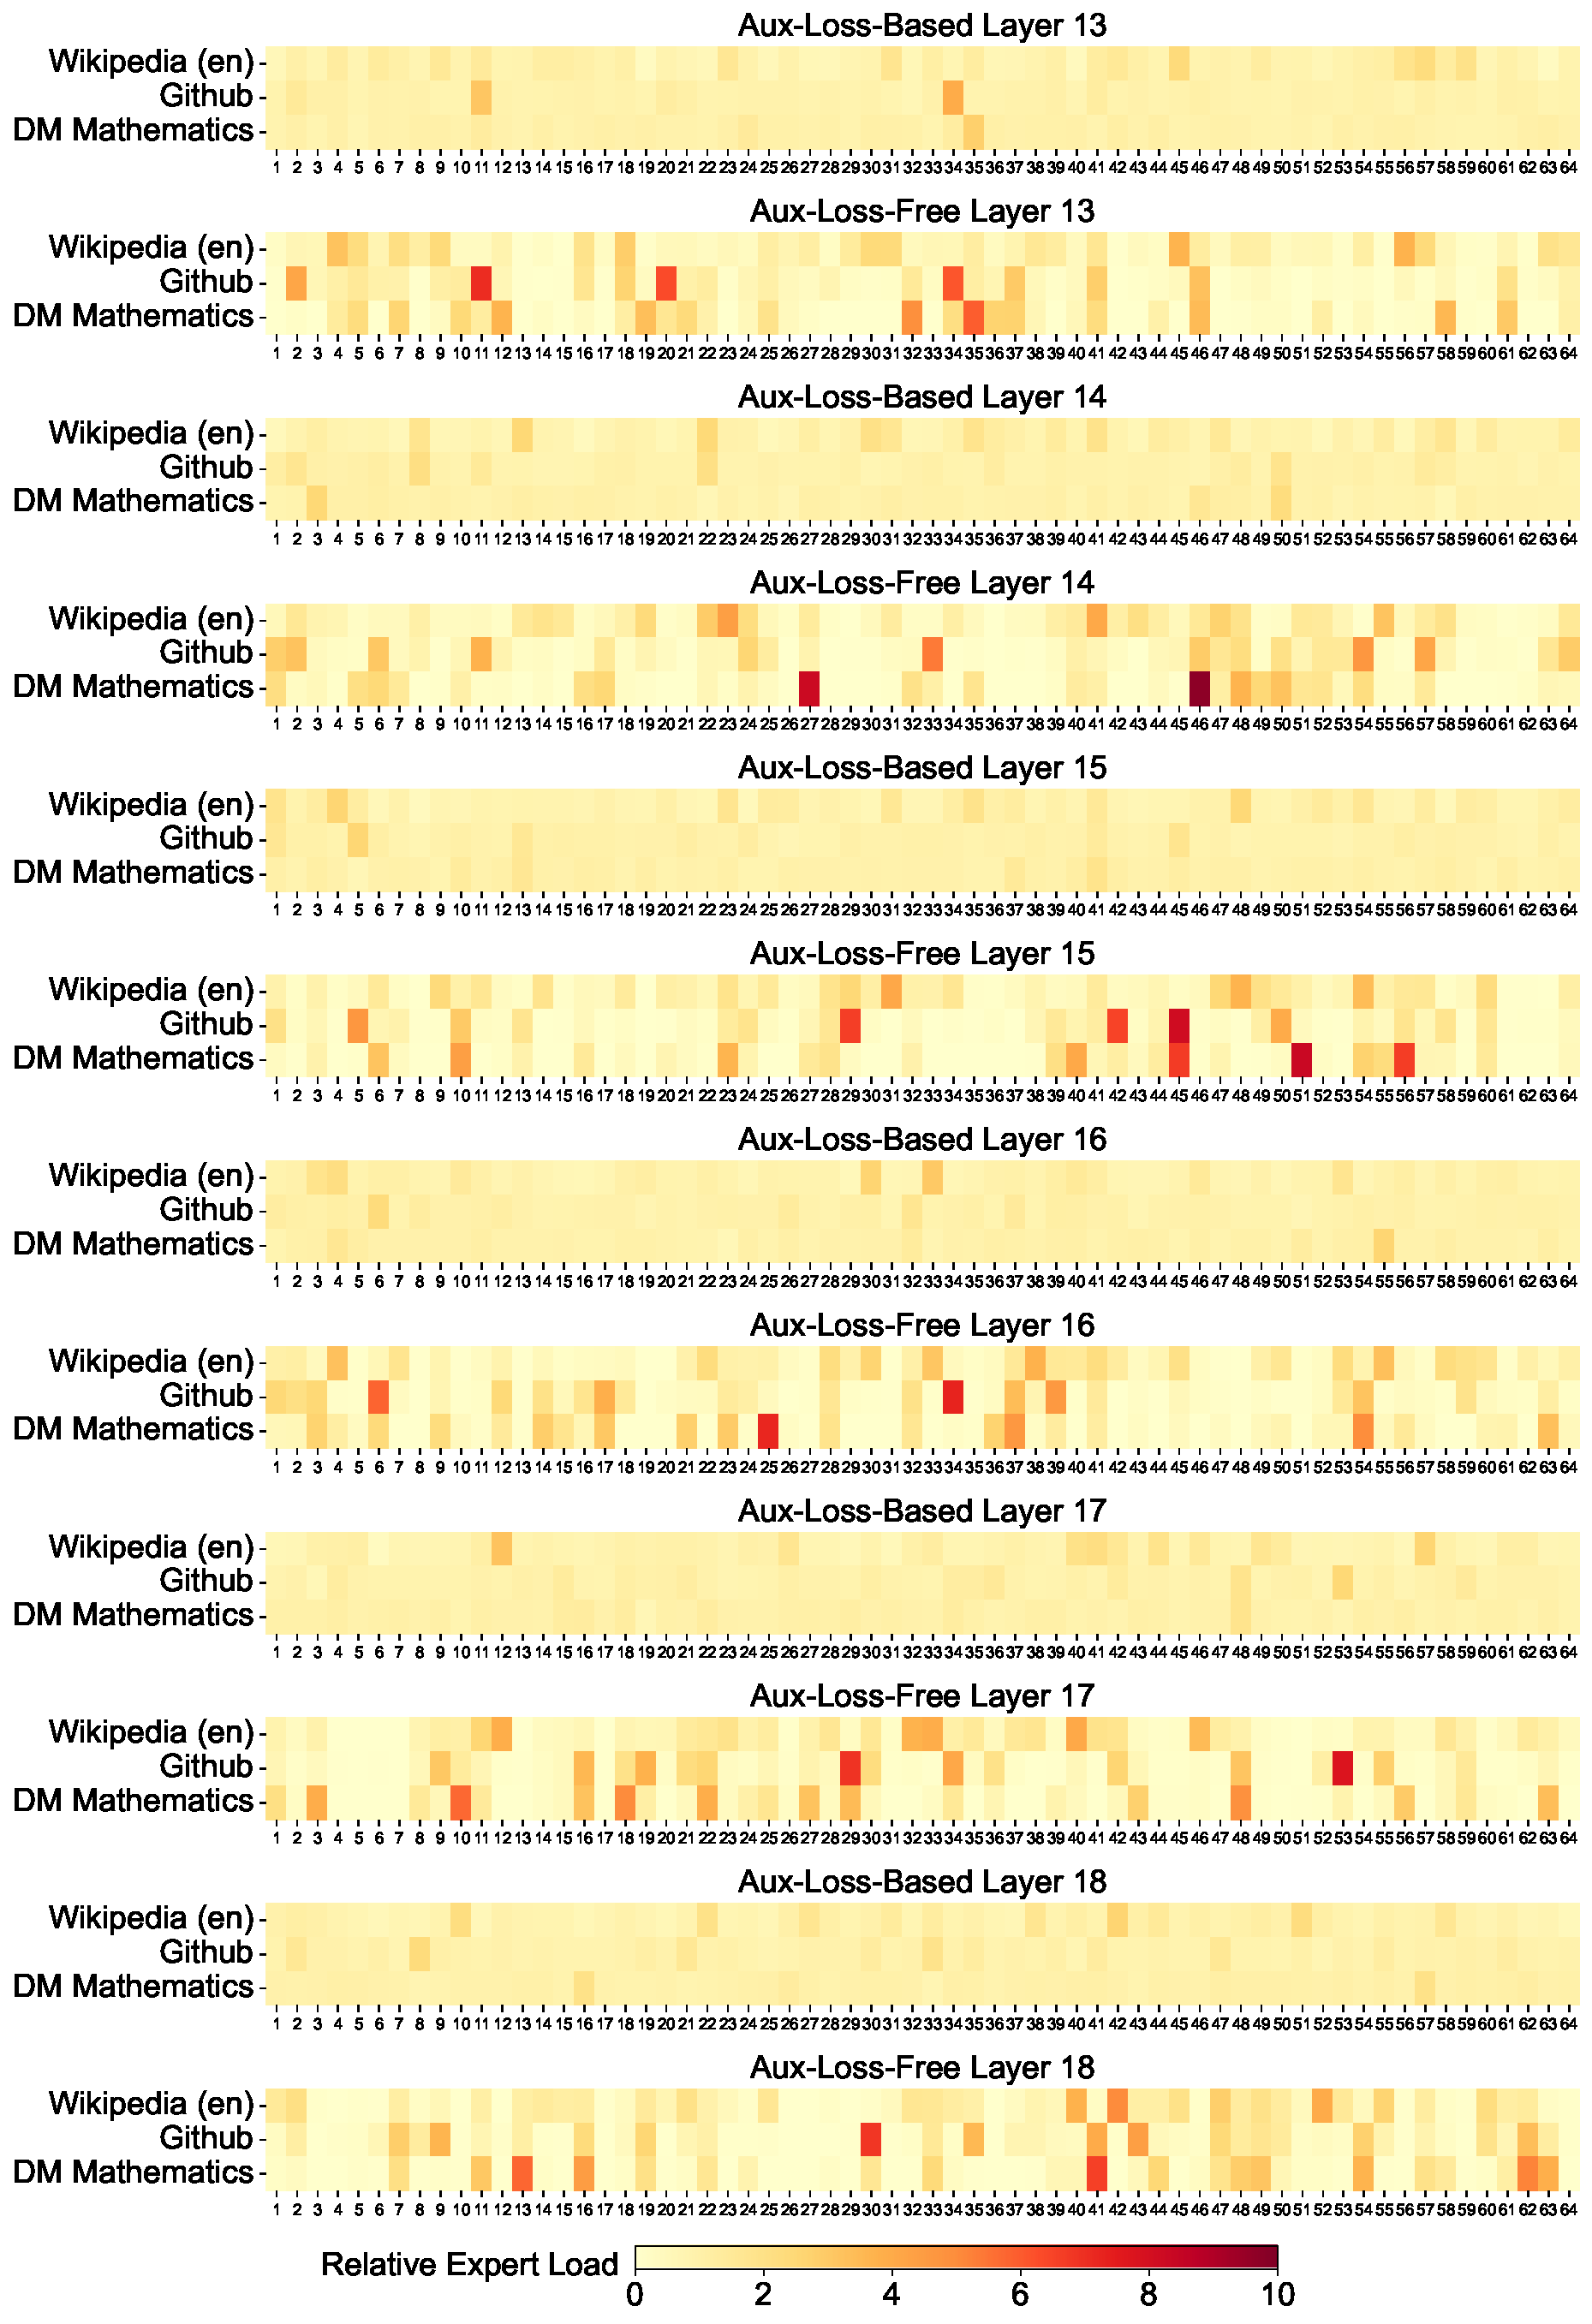
\includegraphics[width=0.95\linewidth]{figures/relative_expert_load_multi_13-18.pdf}
    }
\end{figure}

\begin{figure}[!t]
    \ContinuedFloat
    \subfigure[Layers 19-25]{
        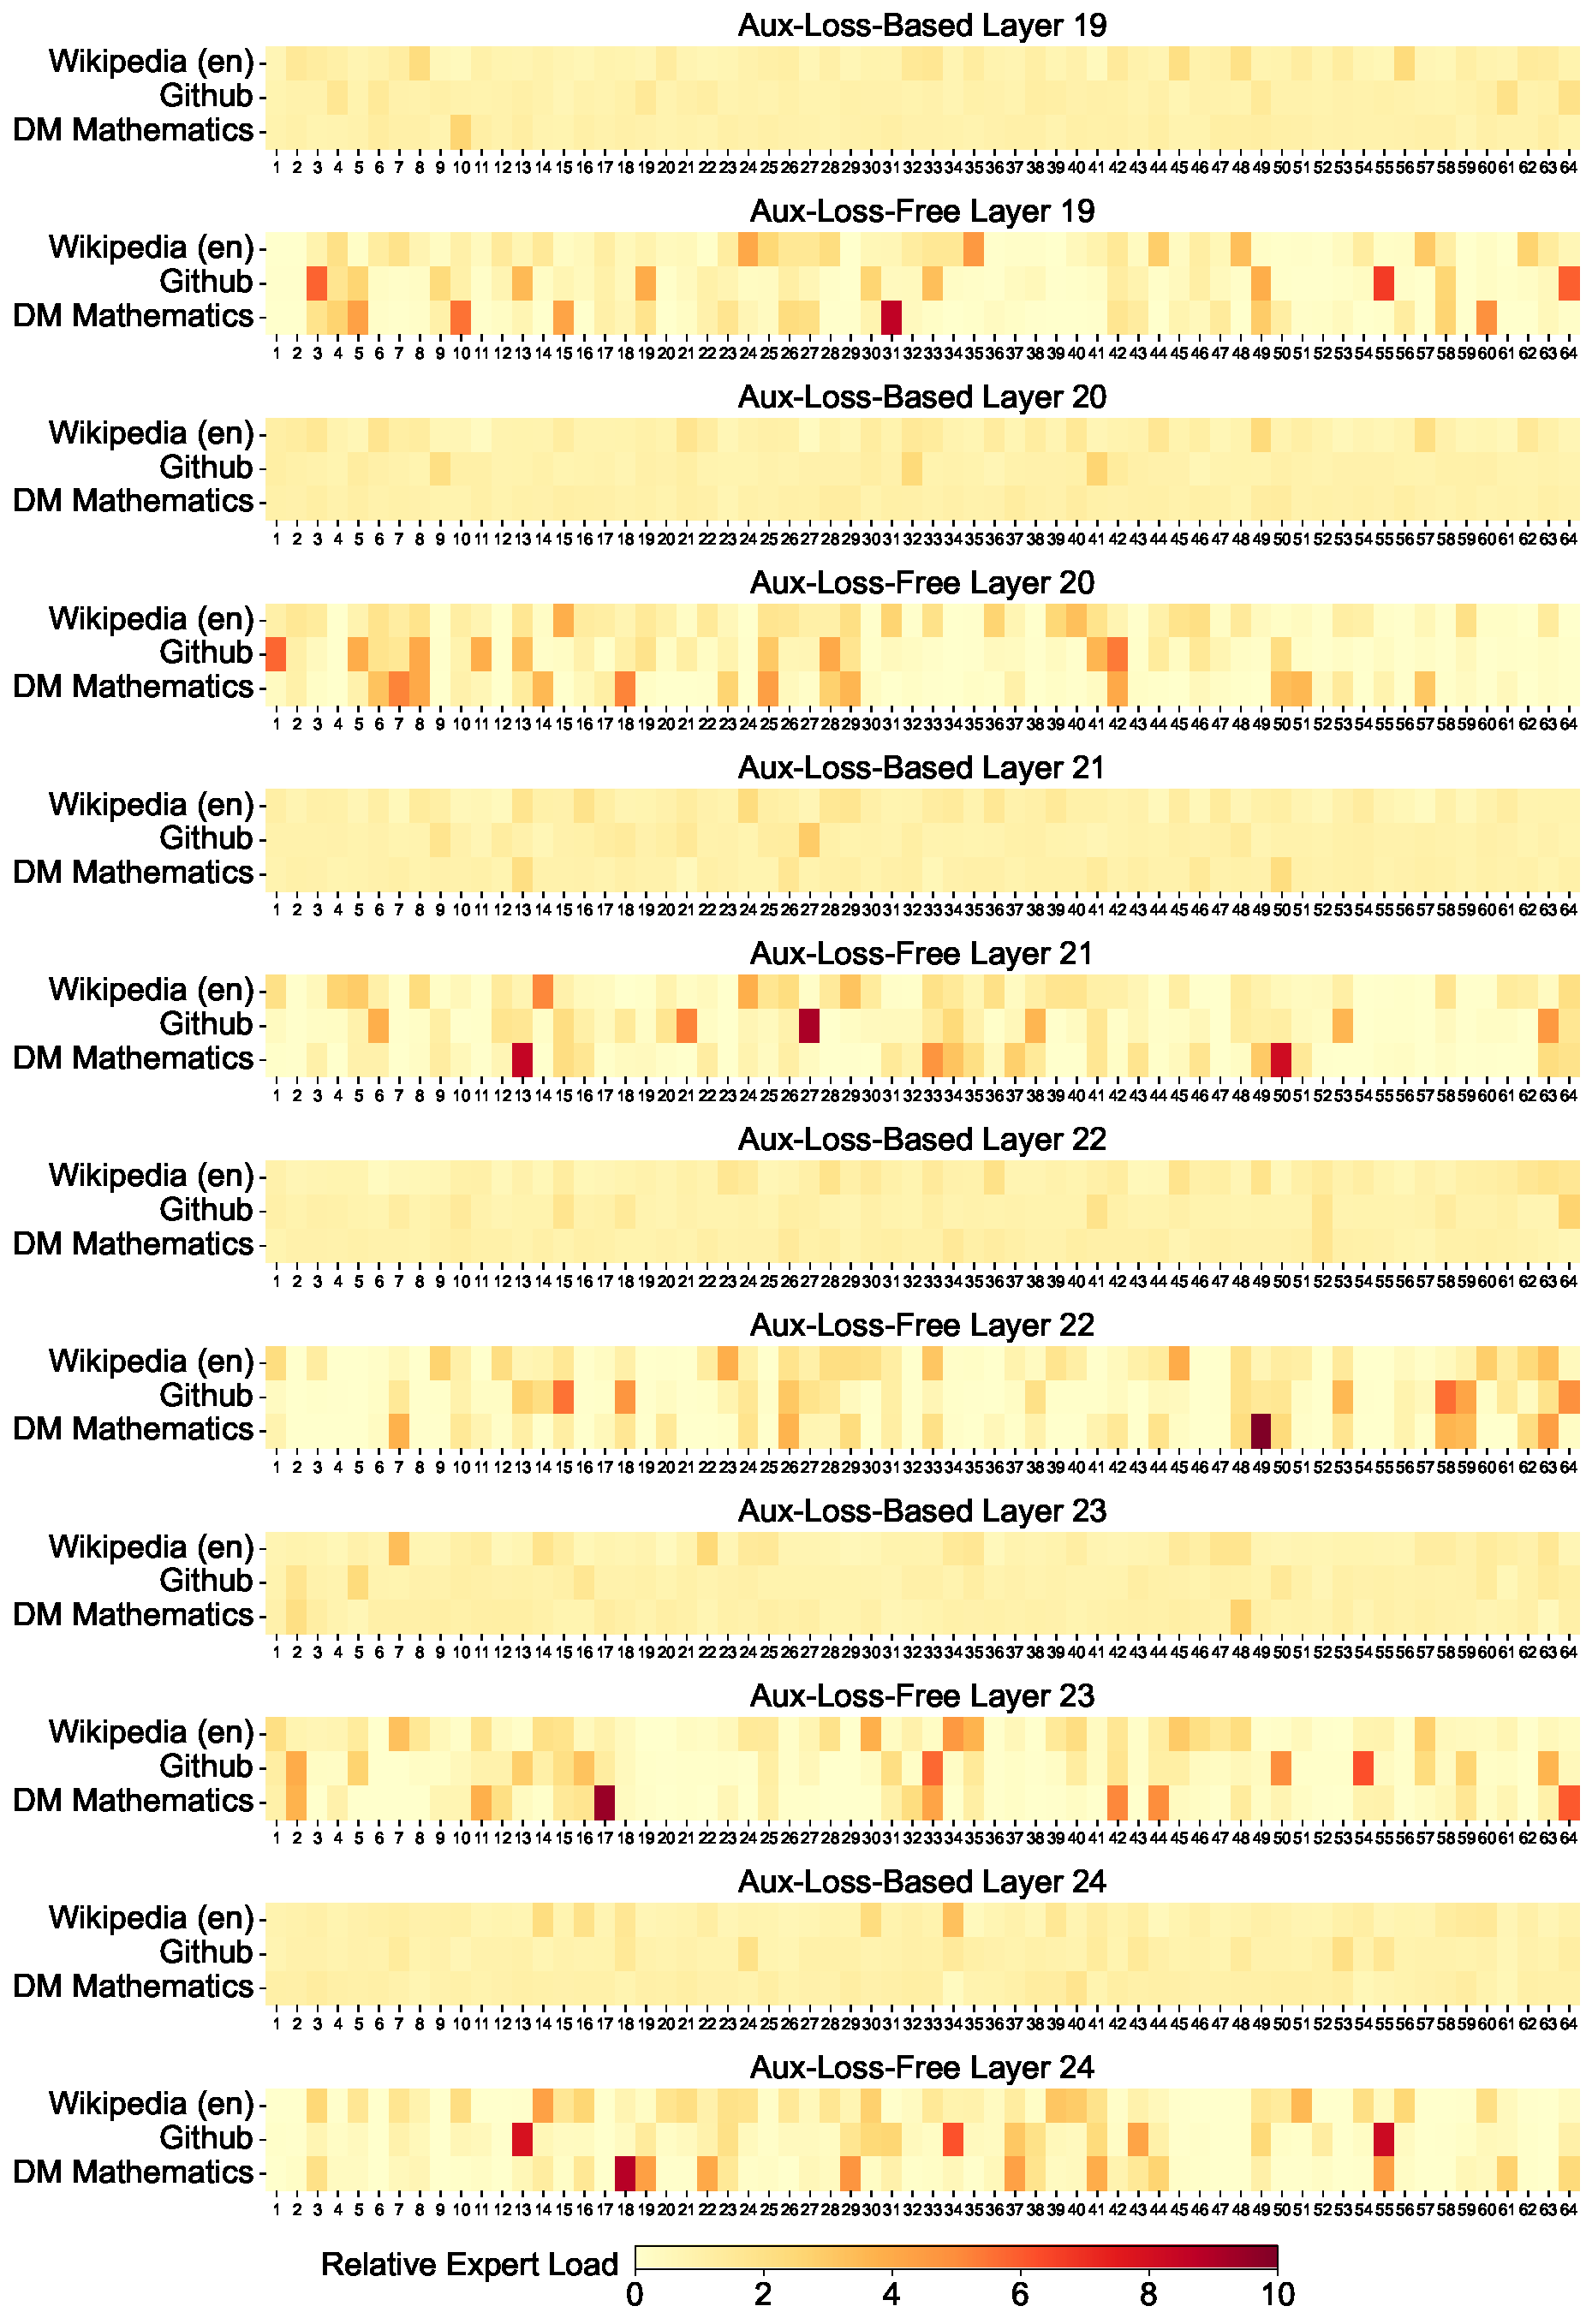
\includegraphics[width=0.95\linewidth]{figures/relative_expert_load_multi_19-24.pdf}
    }
\end{figure}

\begin{figure}[!t]
    \ContinuedFloat
    \subfigure[Layers 25-27]{
        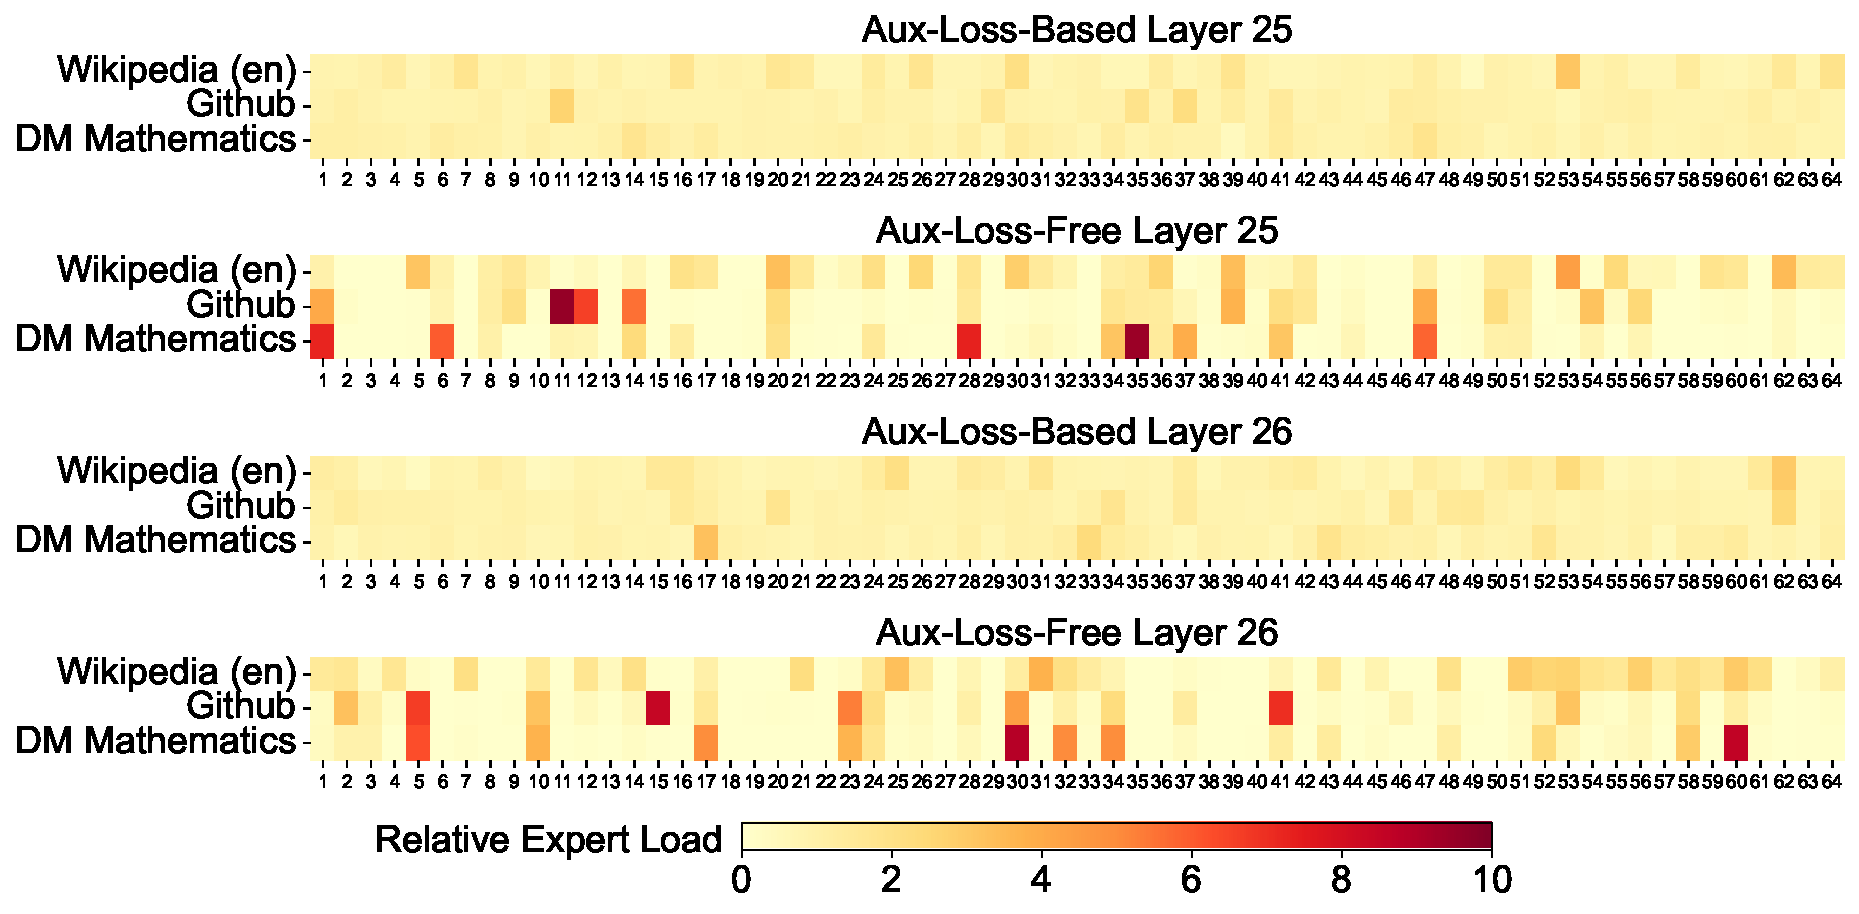
\includegraphics[width=0.95\linewidth]{figures/relative_expert_load_multi_25-26.pdf}
    }
    \caption{
        Auxiliary-loss-free 和 auxiliary-loss-based 模型在 Pile 测试集三个领域上的专家负载。
        Auxiliary-loss-free 模型比 auxiliary-loss-based 模型展现出更强的专家专门化模式。
        相对专家负载表示实际专家负载与理论均衡专家负载之间的比值。
    }
\label{fig:detailed_expert_load}
\end{figure}

\newpage

\end{document}
